\documentclass [11pt,twoside]{article}
\usepackage[utf8]{inputenc}
\usepackage[T1]{fontenc}

%Page margins, header and footer positions
\usepackage{geometry}
 \geometry{
 a4paper,
 total={210mm,297mm},
 left=25mm,
 right=25mm,
 top=30mm,
 bottom=25mm,
 headsep=7mm}

\interfootnotelinepenalty=10000

%To display filling dots in the TOC for all entries
\usepackage[titles]{tocloft}
\renewcommand{\cftsecleader}{\cftdotfill{\cftdotsep}}

%Define new header and footer style
\usepackage{fancyhdr}

\pagestyle{fancy}
\fancyhf{}
\lhead{\color{Gray}{\small{Polaris project by VINCENZO MANTO \& ROBERT MEDVEDEC}}}
\lfoot{\textcolor{Gray}{\small{Copyright © 2022, VINCENZO MANTO \& ROBERT MEDVEDEC – All rights reserved}}}
\rfoot{\textcolor{Gray}{\thepage}}
\renewcommand{\headrulewidth}{0pt}

%PACKAGES
\usepackage{wasysym}
\usepackage{pifont}

\newcommand{\supported}{\ding{52}\xspace}
\newcommand{\unsupported}{\ding{55}\xspace}
\newcommand{\partsupported}{\textcolor{black!40}{\ding{52}}\xspace}
\newcommand{\lowsupported}{\textcolor{black!20}{\ding{52}}\xspace}
\newcommand{\unknowsupported}{\textbf{?}\xspace}

%Font: Times
\usepackage{times}
%Change monospaced font
\renewcommand{\ttdefault}{lmtt}

%tables
\usepackage{tabu}
\usepackage{tabularx}
\usepackage{ltablex}
\usepackage{longtable}
\usepackage{float} % To allow the use of H modifier in long tables

%landscape mode
\usepackage{pdflscape}
\usepackage{rotating}
\usepackage{caption}

%make landscape mode be sensitive to even and odd pages
%start
\def\myrotate{\ifodd\c@page\else-\fi 90}
\makeatletter
\global\let\orig@begin@landscape=\landscape%
\global\let\orig@end@landscape=\endlandscape%
\gdef\@true{1}
\gdef\@false{0}
\gdef\landscape{%
    \global\let\within@landscape=\@true%
    \orig@begin@landscape%
}%
\gdef\endlandscape{%
    \orig@end@landscape%
    \global\let\within@landscape=\@false%
}%
\@ifpackageloaded{pdflscape}{%
    \gdef\pdf@landscape@rotate{\PLS@Rotate}%
}{
    \gdef\pdf@landscape@rotate#1{}%
}
\let\latex@outputpage\@outputpage
\def\@outputpage{
    \ifx\within@landscape\@true%
        \if@twoside%
            \ifodd\c@page%
                \gdef\LS@rot{\setbox\@outputbox\vbox{%
                    \pdf@landscape@rotate{-90}%
                    \hbox{\rotatebox{90}{\hbox{\rotatebox{180}{\box\@outputbox}}}}}%
                }%
            \else%
                \gdef\LS@rot{\setbox\@outputbox\vbox{%
                    \pdf@landscape@rotate{+90}%
                    \hbox{\rotatebox{90}{\hbox{\rotatebox{0}{\box\@outputbox}}}}}%
                }%
            \fi%
        \else%
            \gdef\LS@rot{\setbox\@outputbox\vbox{%
                \pdf@landscape@rotate{+90}%
                \hbox{\rotatebox{90}{\hbox{\rotatebox{0}{\box\@outputbox}}}}}%
            }%
        \fi%
    \fi%
    \latex@outputpage%
}
\makeatother
%end

%graphics
\usepackage{graphicx}
\usepackage[dvipsnames, table]{xcolor}
%If you upload images from PC, you need to insert code for the path here (different for Windows and Unix OS)

%References
%\usepackage{xpatch}
%\usepackage[backend=biber, style=numeric, citestyle=numeric, sorting=none]{biblatex}
%\addbibresource{main.bib}

%Other
\usepackage{ifthen}
\usepackage{xspace}
\usepackage{enumitem}
\usepackage{amssymb}
\usepackage[pdftex, colorlinks]{hyperref}
\newcommand{\comment}[1]{{\color{Red}$\blacktriangleright$ Comment: #1 $\blacktriangleleft$}}


% Some utilities\ldots
\usepackage{soul}
\usepackage{tikz}

\usetikzlibrary{calc}
\usetikzlibrary{decorations.pathmorphing}


\makeatletter

\newcommand{\defhighlighter}[3][]{%
  \tikzset{every highlighter/.style={color=#2, fill opacity=#3, #1}}%
}

\defhighlighter{yellow}{.5}

\newcommand{\highlight@DoHighlight}{
  \fill [ decoration = {random steps, amplitude=1pt, segment length=15pt}
        , outer sep = -15pt, inner sep = 0pt, decorate
       , every highlighter, this highlighter ]
        ($(begin highlight)+(0,8pt)$) rectangle ($(end highlight)+(0,-3pt)$) ;
}

\newcommand{\highlight@BeginHighlight}{
  \coordinate (begin highlight) at (0,0) ;
}

\newcommand{\highlight@EndHighlight}{
  \coordinate (end highlight) at (0,0) ;
}

\newdimen\highlight@previous
\newdimen\highlight@current

\DeclareRobustCommand*\highlight[1][]{%
  \tikzset{this highlighter/.style={#1}}%
  \SOUL@setup
  %
  \def\SOUL@preamble{%
    \begin{tikzpicture}[overlay, remember picture]
      \highlight@BeginHighlight
      \highlight@EndHighlight
    \end{tikzpicture}%
  }%
  %
  \def\SOUL@postamble{%
    \begin{tikzpicture}[overlay, remember picture]
      \highlight@EndHighlight
      \highlight@DoHighlight
    \end{tikzpicture}%
  }%
  %
  \def\SOUL@everyhyphen{%
    \discretionary{%
      \SOUL@setkern\SOUL@hyphkern
      \SOUL@sethyphenchar
      \tikz[overlay, remember picture] \highlight@EndHighlight ;%
    }{%
    }{%
      \SOUL@setkern\SOUL@charkern
    }%
  }%
  %
  \def\SOUL@everyexhyphen##1{%
    \SOUL@setkern\SOUL@hyphkern
    \hbox{##1}%
    \discretionary{%
      \tikz[overlay, remember picture] \highlight@EndHighlight ;%
    }{%
    }{%
      \SOUL@setkern\SOUL@charkern
    }%
  }%
  %
  \def\SOUL@everysyllable{%
    \begin{tikzpicture}[overlay, remember picture]
      \path let \p0 = (begin highlight), \p1 = (0,0) in \pgfextra
        \global\highlight@previous=\y0
        \global\highlight@current =\y1
      \endpgfextra (0,0) ;
      \ifdim\highlight@current < \highlight@previous
        \highlight@DoHighlight
        \highlight@BeginHighlight
      \fi
    \end{tikzpicture}%
    \the\SOUL@syllable
    \tikz[overlay, remember picture] \highlight@EndHighlight ;%
  }%
  \SOUL@
}

\makeatother

% Common abbrev. are set as commands to ensure proper spacing after the dot
\RequirePackage{xspace}
\newcommand{\ie}{i.e.\@\xspace}
\newcommand{\aka}{a.k.a.\@\xspace}
\newcommand{\Ie}{I.e.\@\xspace}
\newcommand{\cf}{cf.\@\xspace}
\newcommand{\Cf}{Cf.\@\xspace}
\newcommand{\eg}{e.g.\@\xspace}
\newcommand{\Eg}{E.g.\@\xspace}
\newcommand{\etal}{et al.\@\xspace}
\newcommand{\etc}{etc.\@\xspace}
\newcommand{\wrt}{w.r.t.\@\xspace}
\newcommand{\Wrt}{W.r.t.\@\xspace}



\date{}


\begin{document}

%TITLE PAGE

\begin{titlepage}


%LOGO

{\begin{table}[t!]
\centering
\begin{tabu} to \textwidth { X[1.3,r,p] X[1.7,l,p] }
\textcolor{Blue}
{\textbf{\small{Design and Implementation of Mobile Applications  - Polaris project VINCENZO MANTO, ROBERT MEDVEDEC}}} & 
\includegraphics[scale=0.5]{Images/PolimiLogo}
\end{tabu}
\end{table}}~\\ [7cm]

%TITLE 

\begin{flushleft}

%Replace the text string with your title
{\textcolor{Blue}{\textbf{\Huge{Design Document}}}} \\ [1cm]

\end{flushleft}

\end{titlepage}

%Define deliverable specific info
%Replace cell contents where needed
\begin{table}[h!]
\begin{tabu} to \textwidth { X[0.3,r,p] X[0.7,l,p] }
\hline
\\
\textbf{Deliverable:} & DD\\
\textbf{Title:} & Design Document \\
\textbf{Authors:} & VINCENZO MANTO, ROBERT MEDVEDEC \\
\textbf{Version:} & 0.1 \\ 
\textbf{Date:} & 02-01-2022 \\
\textbf{Download page:} & \url{https://github.com/robertodavinci/android-dev-travel-app/tree/main} \\
\textbf{Copyright:} & Copyright © 2022, VINCENZO MANTO \& ROBERT MEDVEDEC – All rights reserved \\
\\
\hline
\end{tabu}
\end{table}




\setcounter{page}{2}


%------------------------------------------------------------------------------------------------------------------------------------------------
\newpage
\addcontentsline{toc}{section}{Table of Contents}
\tableofcontents
\newpage
\addcontentsline{toc}{section}{List of Figures}
\listoffigures
\addcontentsline{toc}{section}{List of Tables}
\listoftables

%------------------------------------------------------------------------------------------------------------------------------------------------
\clearpage
{\color{Blue}{\section{Introduction}}}
\label{sect:introduction}
\subsection{Purpose}
\hspace{\parindent}This document provides a detailed description, mainly of the  architecture and the UI, of the 'Polaris' mobile application.\\
'Polaris' application is a system used to enhance travelling experience through idea sharing among people, exploration of other users' travels, documentation and easy manipulation of trip destinations and ideas. The system itself is made so the user has every single information regarding his travel in one place, without having to remember or worry about any details.\\
'Polaris' is mainly a mobile application, with a possibility of being also expanded as a web application in the future.  
\newpage

\subsection{Scope}
\hspace{\parindent}'Polaris' is an application that helps all travellers around the world to easily and efficiently manage their travels and thus enhance their travelling experience. The target audience for this application is everyone who uses a smartphone and has at least some experience in using mobile applications, as some of the patterns and application usages might not be intended for the novices in the field. Thus the target audience ranges from 15 to 50 years old, although there are no strict boundaries.\linebreak


The application is mainly intended to be used when a user is planning and making their own trip and has a liberty to organize their free time and places to visit.\linebreak


Another important usage of the application is sharing trip ideas with friends and other users around the world. Planning trips by itself is a daunting and time consuming task, and with the lack of adequate applications on the market, we wanted to create something that is going to allow users to easily share and modify their previous trips and therefore improve the overall travelling experience for others. 
\break
The most important functions of the application are arranging a trip, finding points of interest in the area, organizing visits to those points, exploring accommodation and restaurants in the area, and crafting your own views of the travel by providing additional comments on the whole experience.


\newpage

\subsection{Definitions, Acronyms, Abbreviations}
\subsubsection{Definitions}
\begin{itemize} 
	\item \textbf{Application}: a computer (mobile) program that is designed for a particular purpose. 
	\item \textbf{Smartphone}: a mobile phone that performs many of the functions of a computer, typically having a touchscreen interface, internet access, and an operating system capable of running downloaded apps. 
	\item \textbf{Google Maps}: a web mapping service developed by Google, used both as a standalone app and as an integrated mapping solution in most of the apps.
	\item \textbf{iOS}: operating system developed by Apple, used by their portable devices like iPads and iPhones.
	\item \textbf{Android}: most popular operating system for smartphones and tablets, developed by Google and partners.
	\item \textbf{Backend}: the part of a computer system or application that is not directly accessed by the user, typically responsible for storing and manipulating data.
\end{itemize}
\subsubsection{Acronyms}
\begin{itemize}
	\item \textbf{API}: Application programming interface, computing interface which defines interactions between multiple software intermediaries 
	\item \textbf{UI}: User interface	
	\item \textbf{GUI}: Graphical user interface
	\item \textbf{DB}: Database
	\item \textbf{REST}: Representational state transfer - software architectural style used in web services
\end{itemize}
\subsubsection{Abbreviations}
\begin{itemize}
	\item \textbf{App}: Application.
\end{itemize}

\newpage
\subsection{Revision History}
\begin{itemize}
	\item \textbf{Version 0.1}: First .tex document created and added all together; 28th December 2021
\end{itemize}

\newpage
\subsection{Reference Documents}
\begin{itemize}
	\item nothing
\end{itemize}



%------------------------------------------------------------------------------------------------------------------------------------------------
\clearpage
{\color{Blue}{\section{Overall Description}}}
\label{sect:desc}
\subsection{Product perspective}
\subsubsection{Technologies overview}
\begin{itemize}
\item Android Studio Development Kit
\begin{itemize}
\item Kotlin
\item Android Compose
\end{itemize}
\item Data management
\begin{itemize}
\item Google Firestore
\item Google Firebase
\item Database
\item Room
\item Shared preferences
\end{itemize}
\item Authentication
\begin{itemize}
\item Google Authentication
\item Facebook Authentication
\item Email Authentication
\end{itemize}
\item External APIs
\begin{itemize}
\item Google Maps
\item Google Translate
\item Google Cloud Messaging
\item Google Places
\item OpenWeatherMap
\item GPT 3 - OpenAI
\end{itemize}
\end{itemize}
\newpage
\subsubsection{Internal structure}
\hspace{\parindent}The proposed system uses an application on the server side that is connected with the APIs to the Android on the phone. 

The Way of communication between the parts of the system and logic behind the system is presented in the following figure:

\begin{figure}[!htb]
\centering
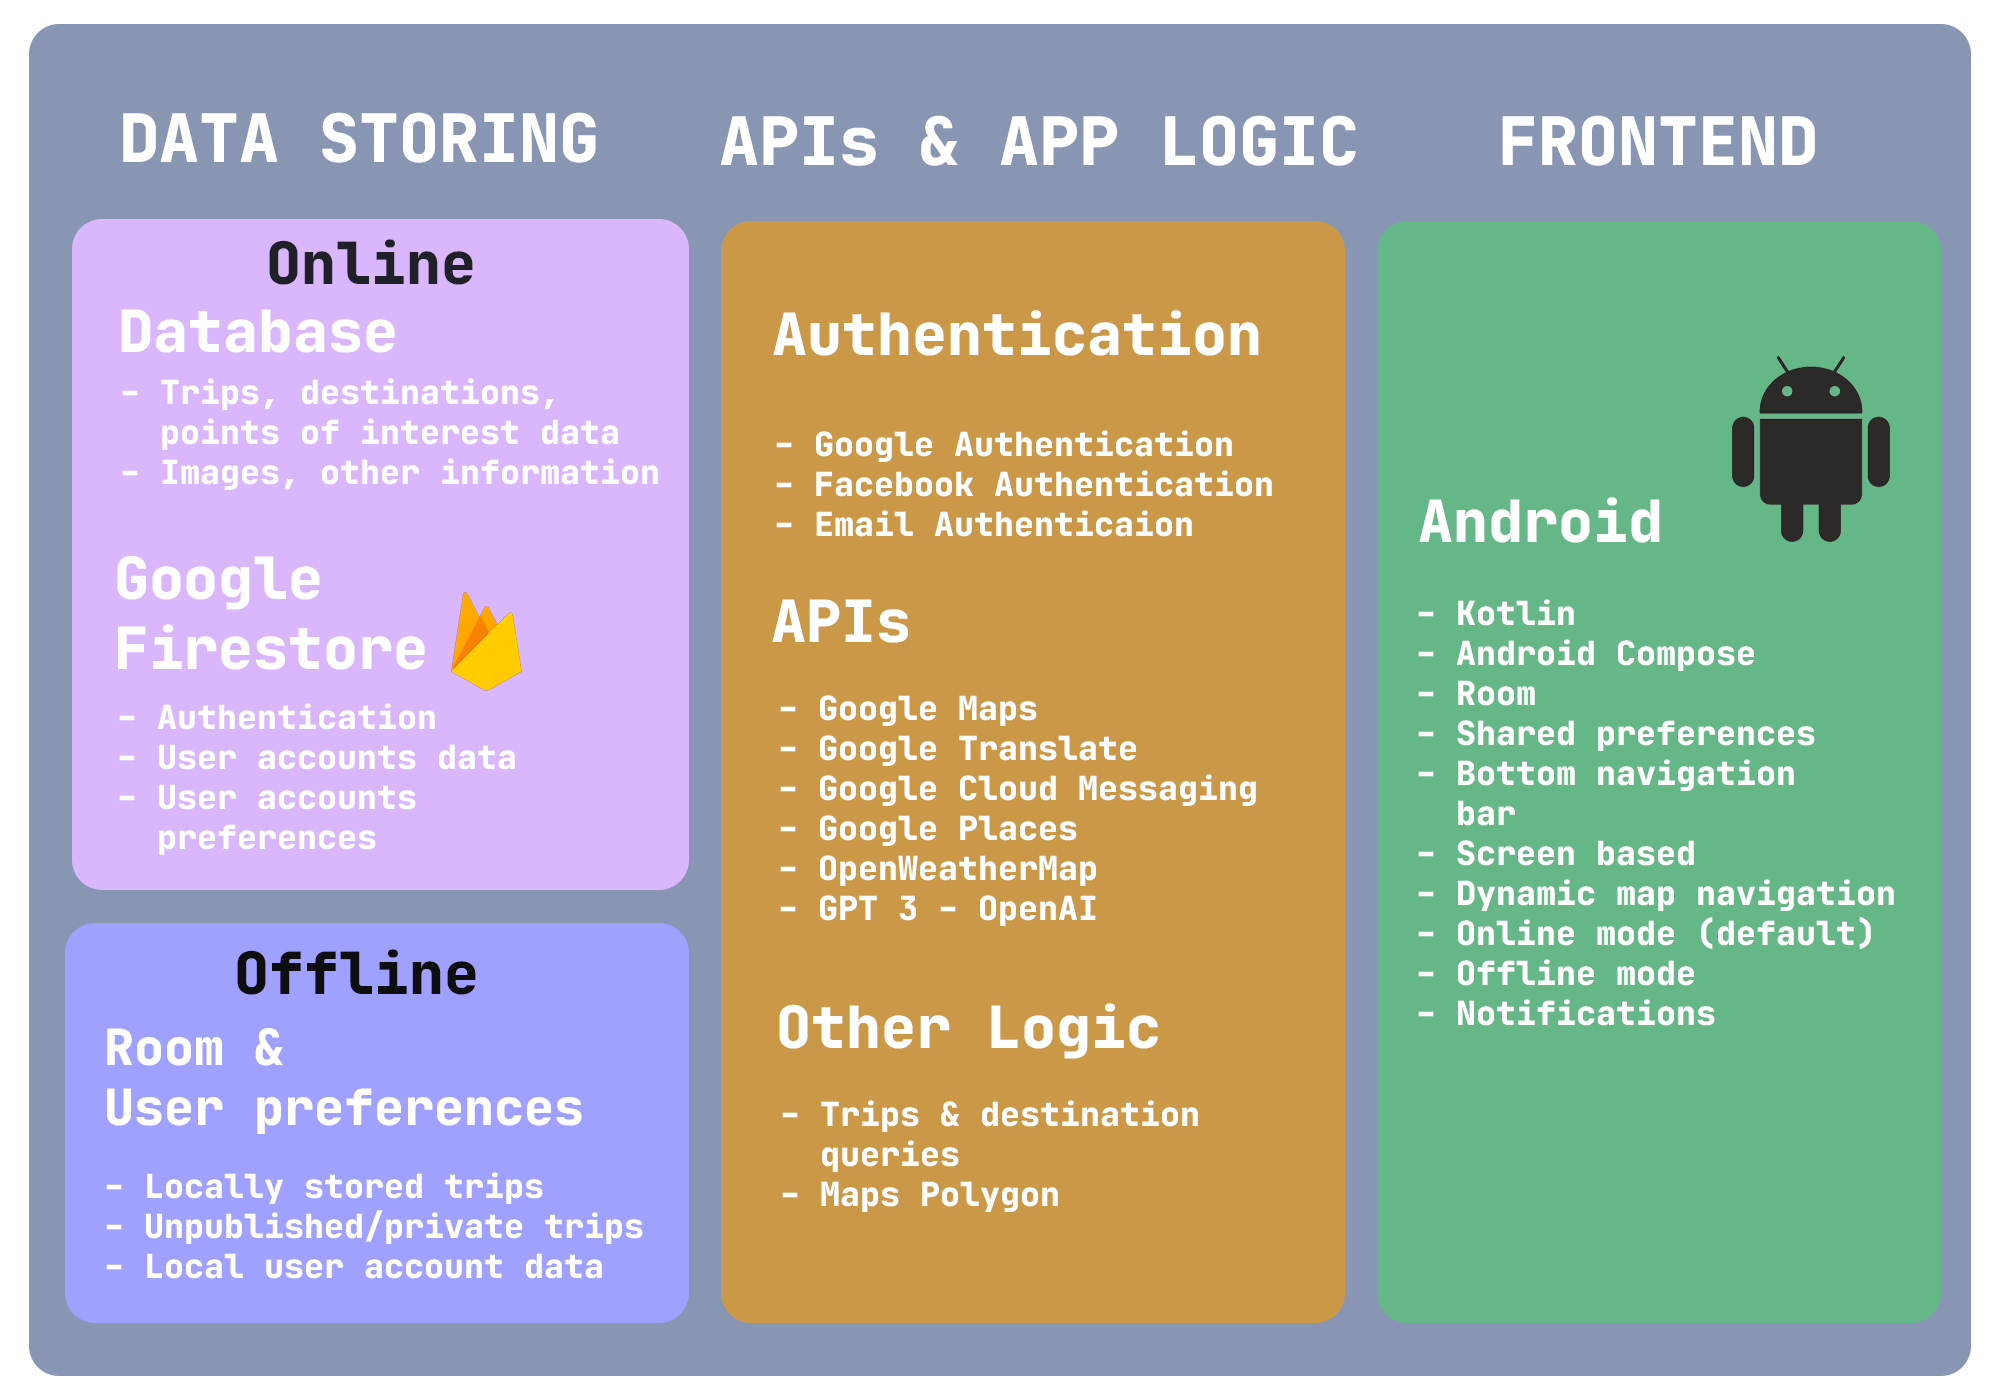
\includegraphics[width=\textwidth]{../Images/InternalStructurePNG_v2.png}
\caption{\label{fig:dbapiuser}\textbf{Internal structure of the system}}
\end{figure}

\textbf{Data storing}\\

The database part is divided into two separate entities. Most of the authentication part is done directly through Google Firebase and Firestore frameworks, which offer great support for Google and Facebook accounts login integration, as well as native support for email based accounts. Controlling authentication via Google services is fast, easy, and seamless, so we have decided to keep most of our logic, as well as account data, stored here. \\ \\
User account details, such as username, ID, and user preferences, are stored in the Google Firestore database, and are fetched after every login, so that the local user account data is consistent with the one on the servers. \\ \\
Images that are used for trips and destinations are also stored in the Google Firestore database.\\ \\
The other part of the database, which stores the data about the destinations, trips, points of interests, and other features related directly to the workflow of the app, are stored in another, separate database. This decision was due to the fact that Google Firestore is a NoSQL database, so putting relational data there would make it inefficient and slow compared to the traditional SQL database.\\ \\
This is what made us decide to transfer this data to completely other place and use a different technology than with the accounts. Account data storing and fetching works exceptionally well and fast with Google services, so we had no real reason to move it from there, especially since that data is more sensitive and Google services provide high level of protection. \\ \\
Android framework also supports numerous features for working locally. We have used these features to have an additional "offline" mode of our application, which allows full functionalities despite the user not having internet connection. We use Android Room to store all the desired trips downloaded and edited by the user, as well as the ones that the user has created locally and decided not to publish yet. "Offline" mode is then synced as soon as the user gets Internet connection, if any additional changes have been made to the local or public trips. \\ \\
Finally, shared preferences are used to store the user's local information such as username, theme preferences, display name, and other features that help user while navigating the app. These are updated with the data located in the Google Firestore framework.\\
\\

\textbf{APIs \& App Logic}\\

Authentication used for the application is done directly through Google Firbase. Account creation can be done directly through email, after which it has to be confirmed via confirmation email. The other way of creating account is logging in with either Facebook or Google account. This way account gets automatically created, or joined if it has already been previously created with the same email. This allows users to not have to worry with which account they have logged in before, as it is all connected to the same email. Users would have to be logged in to either their Google or Facebook account before using those methods to log in to the app.\\ \\
Google and Facebook "button" directly communicate with their respective APIs and only after the conversation has successfully ended do communicate with Google Firebase servers. \\ \\
Another thing that is used from Google framework is the Google Maps API. From that API, several different features are used, such as Maps presentation, location searching, cities searching, distance calculation, and others. Google Maps are dynamically presented in the app and allow users to search through them either by text or by touch.\\ \\
Another important thing is a small PHP script that is running on the server. It serves as a backend of the app, handling query fetching, control, and execution, as well as handling and displaying data that is coming and going through Google Maps API.\\ \\ 
This PHP script is returning all the necessary data in the form of JSON files, which are then handled by the app accordingly and to its needs.

\textbf{Frontend}\\

On the frontend side, we have decided to use all of the latest technologies recommended by Google for Android app development. \\ \\
Kotlin is used as the programming language, which allows better data and variable control in Android environment than the previous official language Java.\\ \\
From the pure design perspective, Android Compose is used instead of the previous template/xml based design. Compose allows for creation of certain elements, as well as their dynamic modelling, which allows for reusability and code cleanliness. Compose allows for elements to by dynamically inserted into specific places, as well as to be dynamically changed, hidden, or manipulated in a much faster and easier fashion. It also allows for faster development since the previews of those compose components can be rendered much faster.\\ \\
As the base of the system, bottom bar with different pages has been used. More on that part is explained in latter chapters of this document.
\\ \\ 
The app supports both online and offline mode, with shared preferences used for storing local display preferences of the app.\\ \\
\newpage

\subsubsection{Scenarios}

\textbf{Scenario 1}\\

\hspace{\parindent}Marco wants to go to a trip to France. His friend, Federico, already went on a trip in a similar area and visited points of interest that Marco likes. Marco asked Federico to tell him all of the places he visited, how did he travel, and the order in which he visited these places. Federico made some notes for Marco, but it still left Marco with the problem of having everything in his phone organized and in one place. That's when Marco found out about the app and asked Federico to put everything he remembers from the trip here. That way Marco had all of the locations in the correct order, as well as comments about certain places and other detailed information all in one place, which allowed him to easier follow the trip during his time in France.\\

\textbf{Scenario 2}\\

\hspace{\parindent}Rebecca, the friend of Marco and Federico, heard about their trip to France and decided to go there as well. However, she is not as interested into visiting so many French castles like Marco and Federico, and wants to add some other destinations to her trip. However she still wants to keep the first half of the trip, where guys visited the southern part of France. She also uses the app and copies the trip, after which she edits it and replaces castle destinations with beaches on the northern part of the country. She renames the trip and publishes it with a different name. This way Rebecca saved some time and effort on planning the entire first half of the trip, whilst being able to modify the experience in the latter half.\\

\textbf{Scenario 3}\\

\hspace{\parindent}Giovanna wants to on a trip but she already visited France. She needs some new ideas. By using the "explore" function in the app she finds some of the top rated trips around Europe - her favourite of those is a trip to Iceland. Giovanna follows all of the guidelines in the trip and has an amazing time.\\

\subsection{Product functions}
\hspace{\parindent}Functions of the system provide easy and intuitive ways to use the app. They are somewhat connected and have overlapping features. Nevertheless, the users may use only certain parts of the system and still get the full functionality they need from the app.
These functions are mentioned in several places in the document, but their most thorough explanation can be found here.
\subsubsection{Adding a trip}
\hspace{\parindent}Adding a trip is the most essential part of the system. The function features several parameters and allows for high level of customizability in order to create a fully unique travel experience. \\
Each point of interest is featured as a specific "destination", although even places that are not regarded as specific destinations can be inserted into a trip. Destination fetching is done through the Google Maps API, with the users also having the ability to add and edit their own destinations.
The function features the following:
\begin{itemize}
\item Selecting a starting point, that is then connected to the nearest city on the map
\item Adding other destinations to the trip
\item Writing a trip description
\item Adding preferred way of travel between destinations
\item Identifying trip price level
\item Adding comments to trip destinations
\item .............
\end{itemize}
\subsubsection{Editing a trip}
\hspace{\parindent}Editing a trip can be done on two different types of trips - public or private. If the trip is public, either published by the user editing it or someone else, by starting to editing an exact copy of that trip is created, which can then be published again under different name and different trip ID.\\
If the trip is private and has not yet been published, then a new trip is not created, but rather the trip ID stays the same. If the trip is then published and edited again, the new edited version of the trip has a new trip ID and is a whole new entity.\\
Editing a trip features all of the same functions that adding a trip does, which means that everything from a small comment to the whole trip can be changed. 
\subsubsection{Finding a trip}
\hspace{\parindent}Finding a trip can be done in several different ways. The first way features a search bar which then searches a trip by the starting point name or by the city which is the closest to that destination. The second way is a search by the trip ID or a hyperlink, which can be directly received from other users. The third way is by accessing a specific user's account page and scrolling through their published trips. Finally, trips can also be found by looking at the interactive map, selecting the area of the desired starting point of the trip, and finding the trip through the distinct trip name and photo.  
\subsubsection{Following a trip}
\hspace{\parindent}This function mainly uses a specific trip and sets it as an active trip of the user. This makes it easily accessible by the user at all times by using the bottom navigation bar, and allows him to follow certain steps of the trip without losing progress. This function also allows the user to change the current active trip and still keep the progress of an old trip, so that the progress can be easily restored when that trip is again set as an active trip.
\subsubsection{Updating account settings}
\hspace{\parindent}Only a few settings can be changed in the user account. List is the following:
\begin{itemize}
\item Changing a username
\item Changing a profile picture
\item Switching between dark and light colour scheme
\item Setting preferred price level
\item Switching between offline mode and online mode
\end{itemize}
\subsubsection{Offline function}
\hspace{\parindent}The system allows the users to be disconnected from the Internet and still use the app fully. Individual trips can be downloaded and store in the phone internal storage, and then accessed at any time. If any changes are made to the trip during the offline time, a new iteration of the trip gets created and published as soon as the connection is restored and the user has come back to the online mode. Multiple trips can be downloaded and kept in the storage of the phone at all times.  




%------------------------------------------------------------------------------------------------------------------------------------------------
\clearpage
{\color{Blue}{\section{Architectural Design}}}
\label{sect:arch}
\subsection{Overview}
\hspace{\parindent}Architectural design of the application is based on the three-layer model used in most applications. The three layers are the presentation layer, or frontend, the application layer, or middleware, and the data layer, or backend. Each of those layers does its own part of the job and communicates with other layers in order to present the correct information to the user.\\
The architecture is also a typical client-server implementation where server holds the data and the client is accessing it through requests (besides the offline mode where the user stored some of the data from the server locally and is accessing it without using online requests).\\
\subsubsection{Backend architecture}
\textbf{User database}\\

As previously mentioned, user database is located in the Google Firestore service. This service uses real-time NoSQL database. This database is organized in collection->document system. Everything starts with one collection, which can hold as many documents (entities) as possible. Each document can have an unlimited number of attribute fields, which can be with a specified type or without one, and at most one collection. Then the cycle repeats again.\\ \\
Working with NoSQL has its advantages when it doesn't have a lot of relational and connected data. We can extract only the small amount of data we want, it is very fast, and also very efficient. Since accounts are not connected in any way, using NoSQL database  seemed like a viable choice since it saves our users time and data. \\ \\
The architecture of this database is the following: the first collection contains all the users as their unique IDs, where they are represented by a document. The first level of the document holds only the info of the display name and the ID.  The second collection is made for storing user preferences, and every user has their own. In that collection there is a document that holds all of the parameters needed for the user's usage of the app, such as colour mode, economy level, thumbnail URL; and two optional ones, real name and real surname
\\ \\
The following figure represents the structure of the explained database.\\
IMAGE OF THE NoSQL architecture


\subsubsection{Middleware architecture}
In order to connect the data on the server to the screen of the phone and to allow the user to properly see the data, we have implemented a complicated layer of functions and classes in order to create easy-to-use and esthetically pleasing experience for the user.

\subsection{Runtime view}

In the following section, sequence diagrams that represent the most important use cases are shown and explained in detail. We have focused only on the most commonly used use cases in the app, as well as their crucial parts. We do not go into too much detail when it comes to specific parts of interaction between the layers, but rather want to present the vague idea and how it all works.

\subsubsection{Create a trip}

Create a trip use case starts with opening the app and pressing on the "Create a trip" button. A new screen opens up which allows us to change certain attributes about the trip and add different destinations. Every trip needs to have a name, which doesn't have to be unique, since there is an ID that is automatically allocated to the every trip. Every trip needs to have at least two destinations. We can search through destinations via the search bar or by using the interactive map and selecting a destination from the map. After selecting a destination, we add it to the trip. Destinations can be reordered and removed from the trip at any time, which is not shown in the diagram due to simplicity and concision. The price level of the trip should also be defined before saving the trip. Trip can also be discarded. In the end, if the user is satisfied with its trip, they can publish it in which case it will be stored directly in the database. Local database is not used for storing unpublished trips, since this would mean that by losing local data, all of the unpublished trips would be lost. All of the trips are stored in the online database and are can be found by other users only if published.  

IMAGE OF CREATE A TRIP

\subsubsection{Edit a trip}

Edit a trip use case starts with opening the app and choosing one of two ways of searching for a trip. One way is searching for a trip name/ID directly through the search bar, and another is by searching for a trip on the interactive map. After the trip is found, it is somewhat "copied" to the instance of the user. User can then edit every single bit of the trip - change the name, change the price level, and add/remove destinations (again, destination removal is not shown in the graph due to simplicity). Finally the user can choose to save the trip without publishing it, or publish it so that everyone else is able to find it. Either way, the trip gets a brand new ID only if it has been changed in any way (changing only the trip name and/or price level is not regarded as a change). Again, due to data safety, in either case it is stored online.

IMAGE OF EDIT A TRIP

\subsubsection{Add a destination}

Add a destination use case starts with opening the app and choosing one of two ways of adding destination - either by using the dynamic Google Maps API, or by using a search function which searches for specific places and locations in the Google database. By using a Google Maps way, the user can specify the exact location, while by using the search way, the user can pick of the previous existing locations in the database. After picking a location, the user can change a name and/or add an specific image of this location. This way the user is allowed to personalize locations for their trip needs. After saving all of the data in the form of a destination, the new destination is published and can be found by other users and added to their trips. There are no local and unpublished destinations.

IMAGE OF ADD A DESTINATION

\subsubsection{Search for a trip/explore}

\subsection{Testing}


%------------------------------------------------------------------------------------------------------------------------------------------------
\clearpage
{\color{Blue}{\section{User Interface Design}}}
\label{sect:ui}
\subsection{Identity and colours}
\hspace{\parindent}The official name of the app is 'Polaris'. The app identity is an astronaut, with the idea of a user acting as an astronaut, which has an overview of the planet Earth and can just pick a place and travel wherever. This feature is also presented in one of the screens in the app, as user searches for already existing trips by searching the globe.

\begin{figure}[!htb]
\centering

\includegraphics[width=0.4\textwidth]{../Images/PolarisIcon.png}
\caption{\label{fig:dbapiuser}\textbf{'Polaris' icon featuring an astronaut on a blue background}}
\end{figure} 

The main colours used for the app are two slightly different blues. Primary blue has the RBG value of \#0083FF while secondary blue has the RBG value of \#0460D9. They are used interchangeably throughout the app.
\begin{figure}[!htb]
\centering
\begin{minipage}{.45\textwidth}
\centering

\includegraphics[width=.5\textwidth]{../Images/UI/primaryColor.png}
\caption{\label{fig:dbapiuser}\textbf{Primary color \#0083FF}}
\end{minipage} 
\begin{minipage}{.45\textwidth}
\centering
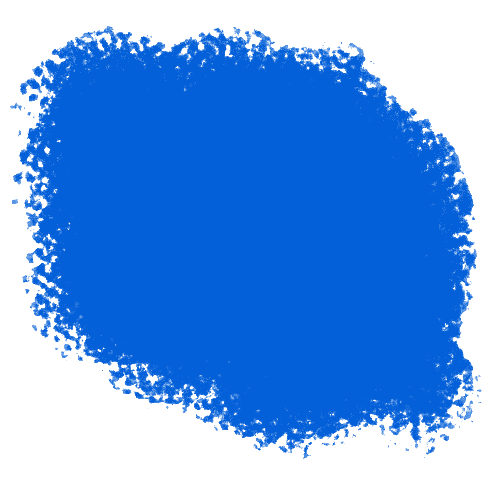
\includegraphics[width=.5\textwidth]{../Images/UI/secondaryColor.png}
\caption{\label{fig:dbapiuser}\textbf{Secondary color \#0460D9}}
\end{minipage}
\end{figure} 

As app features both light and dark mode, there are also colour palettes used for those instances. The same primary and secondary colours are used for accents, but for backgrounds and texts, the colours presented in the following two figures are used. 

\begin{figure}[!htb]
\centering
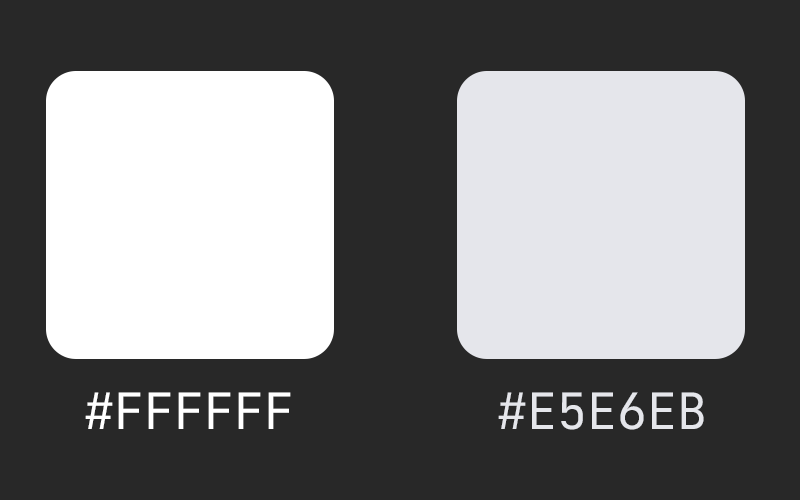
\includegraphics[width=0.7\textwidth]{../Images/UI/BackgroundLight.png}
\caption{\label{fig:dbapiuser}\textbf{Background colours for light theme}}
\end{figure} 

\begin{figure}[!htb]
\centering
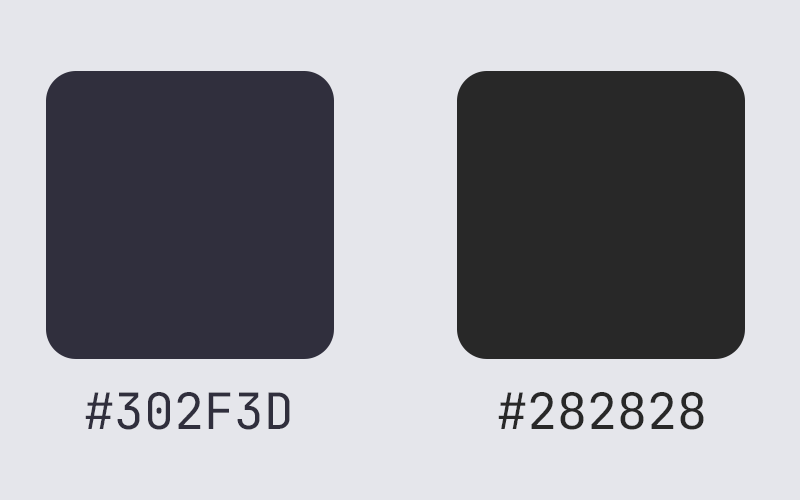
\includegraphics[width=0.7\textwidth]{../Images/UI/BackgroundDark.png}
\caption{\label{fig:dbapiuser}\textbf{Background colours for dark theme}}
\end{figure} 
\newpage

\subsection{User interface design}

\hspace{\parindent}This section features the main design choices of the entire UI of the app, which includes navigation bars, menus, buttons, and other choices. It will not go into too much detail about every component, as all of the screens will be shown with a short comment about it. \\ \\
The main part of the app is divided into four major components, with additional screens available for other functionalities, such as adding and editing destinations and trips. At the bottom of the app there is a navigation bar that leads the user to all of the main screens. Additionally, users can navigate to the settings/account screen either by pressing the 'Polaris' icon in the upper right corner of the screen, or by pressing the last icon in the bottom navigation bar. Right above the navigation bar, a search bar is located which allows the users to search for their previously saved trips.\\ \\
As previously mentioned, the app features both light and dark themes. The following figures present the same screens for both of the themes.\\


\subsubsection{Main screen}

\begin{figure}[!htb]
\centering
\begin{minipage}{.48\textwidth}
\centering
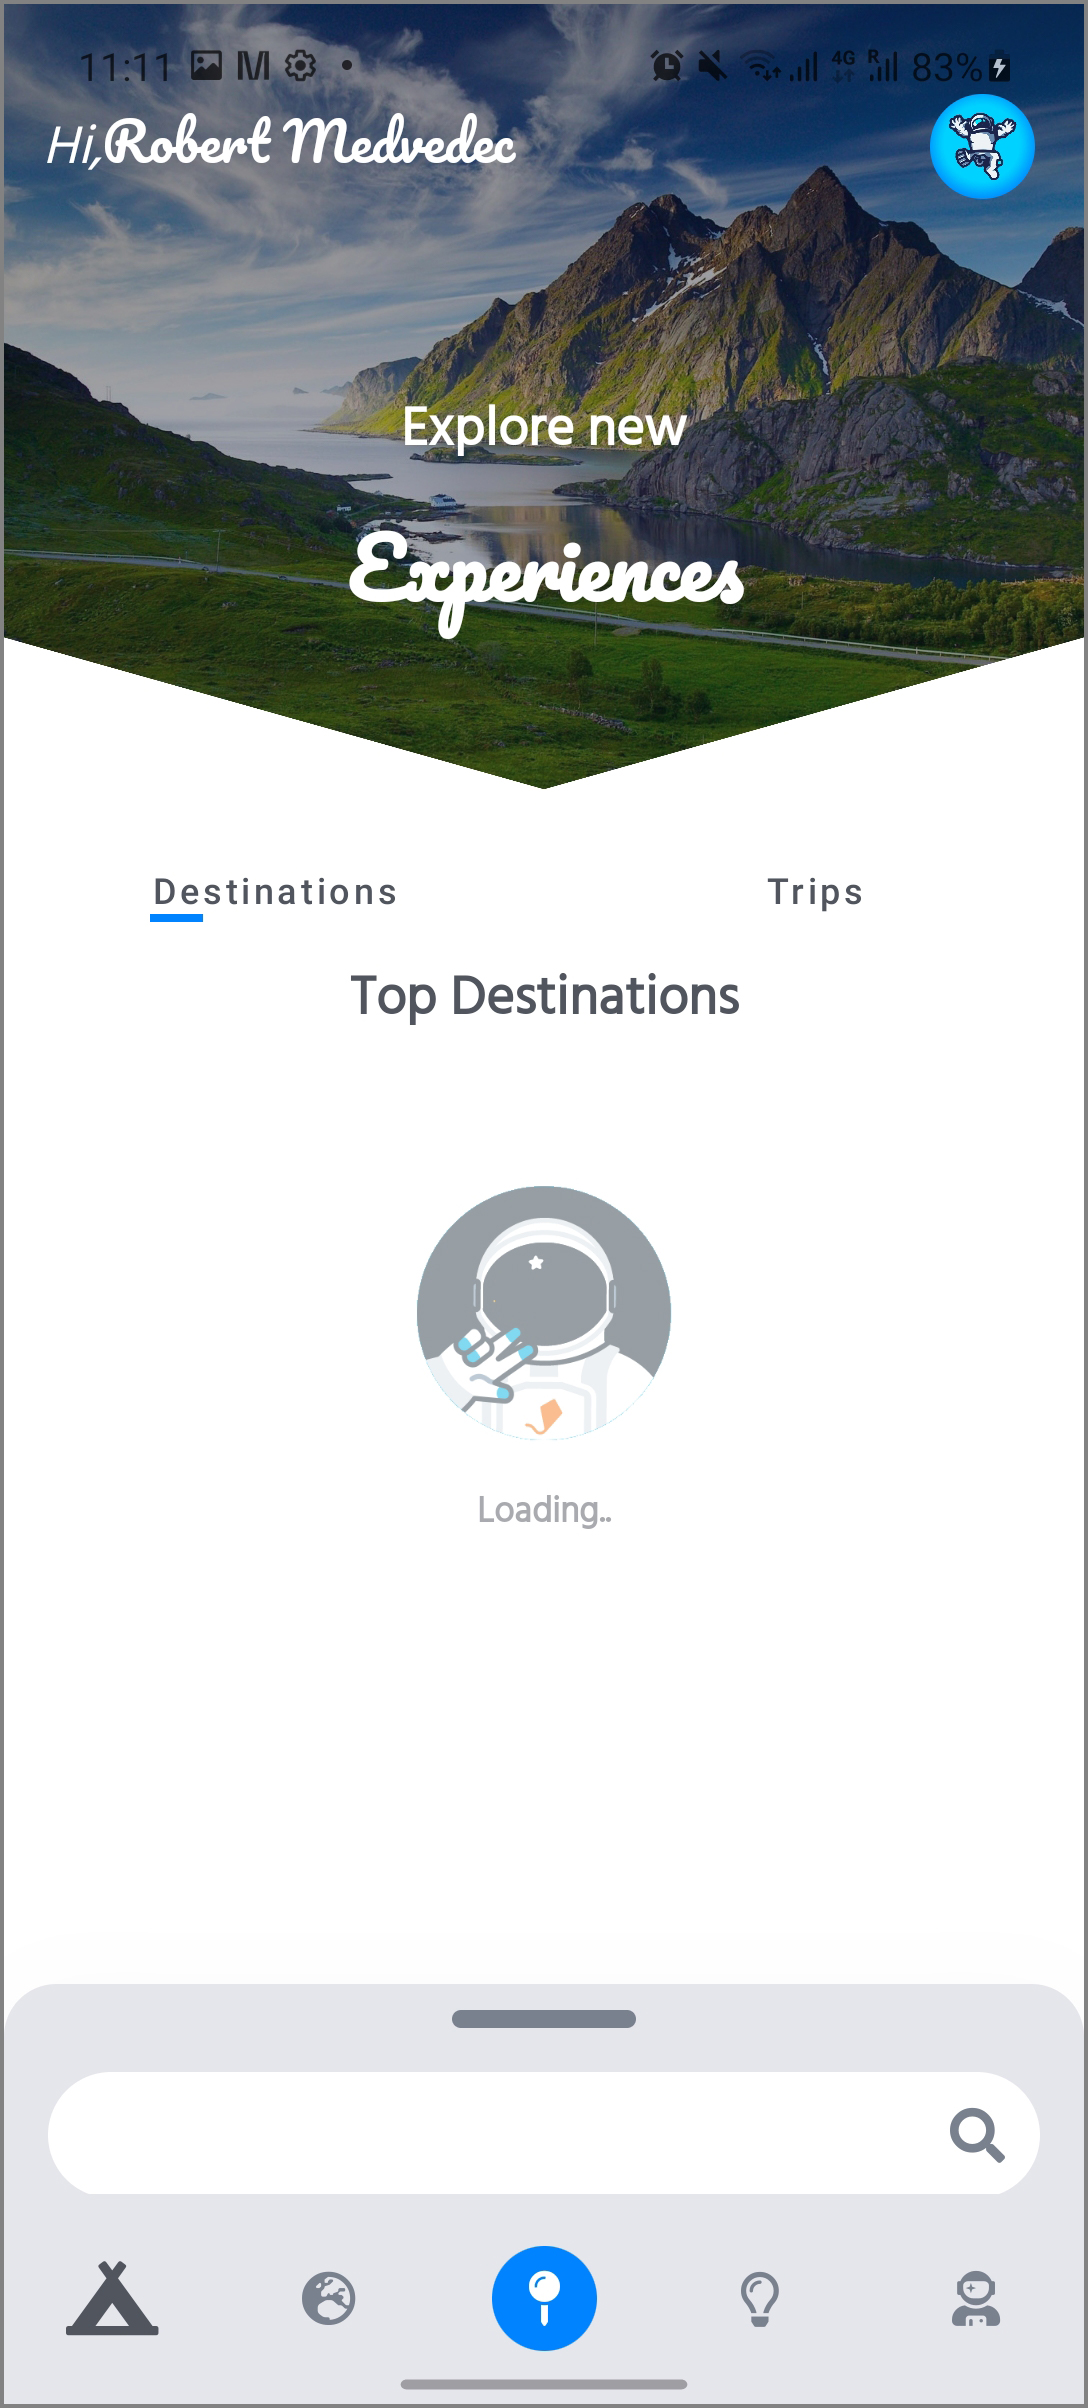
\includegraphics[width=.9\textwidth]{../Images/UI/MainLight.jpg}
\caption{\label{fig:dbapiuser}\textbf{Main screen in light style}}
\end{minipage} 
\begin{minipage}{.48\textwidth}
\centering
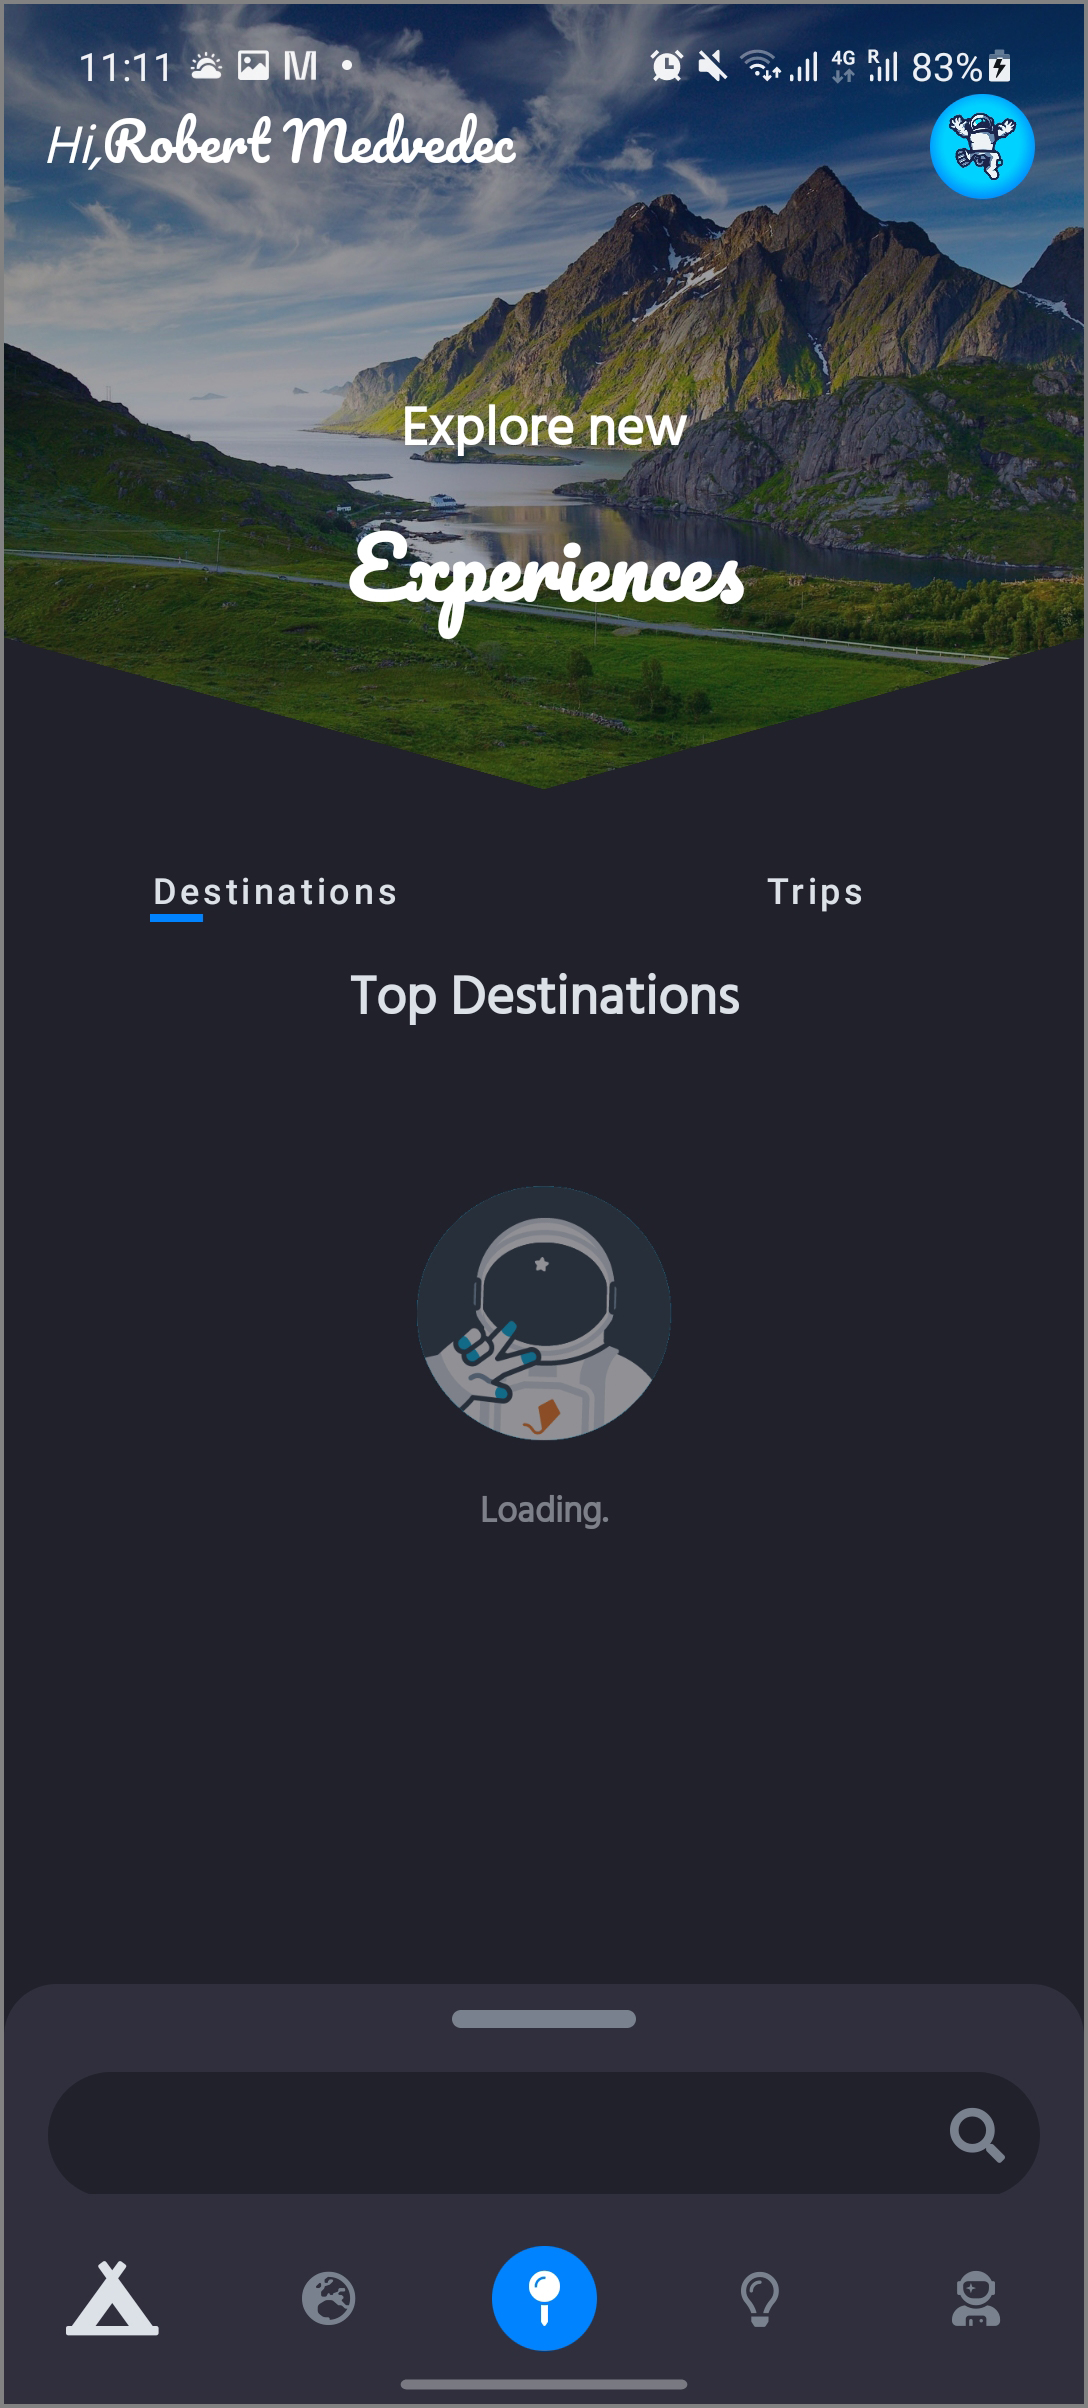
\includegraphics[width=.9\textwidth]{../Images/UI/MainDark.jpg}
\caption{\label{fig:dbapiuser}\textbf{Main screen in dark style}}
\end{minipage}
\end{figure} 

Main screen provides user with the information about the existing destinations and trips. It offers the user a fast way to access some of the information about the locations that they might find useful to build on or to explore.
\newpage
\subsubsection{Map screen}
\begin{figure}[!htb]
\centering
\begin{minipage}{.48\textwidth}
\centering
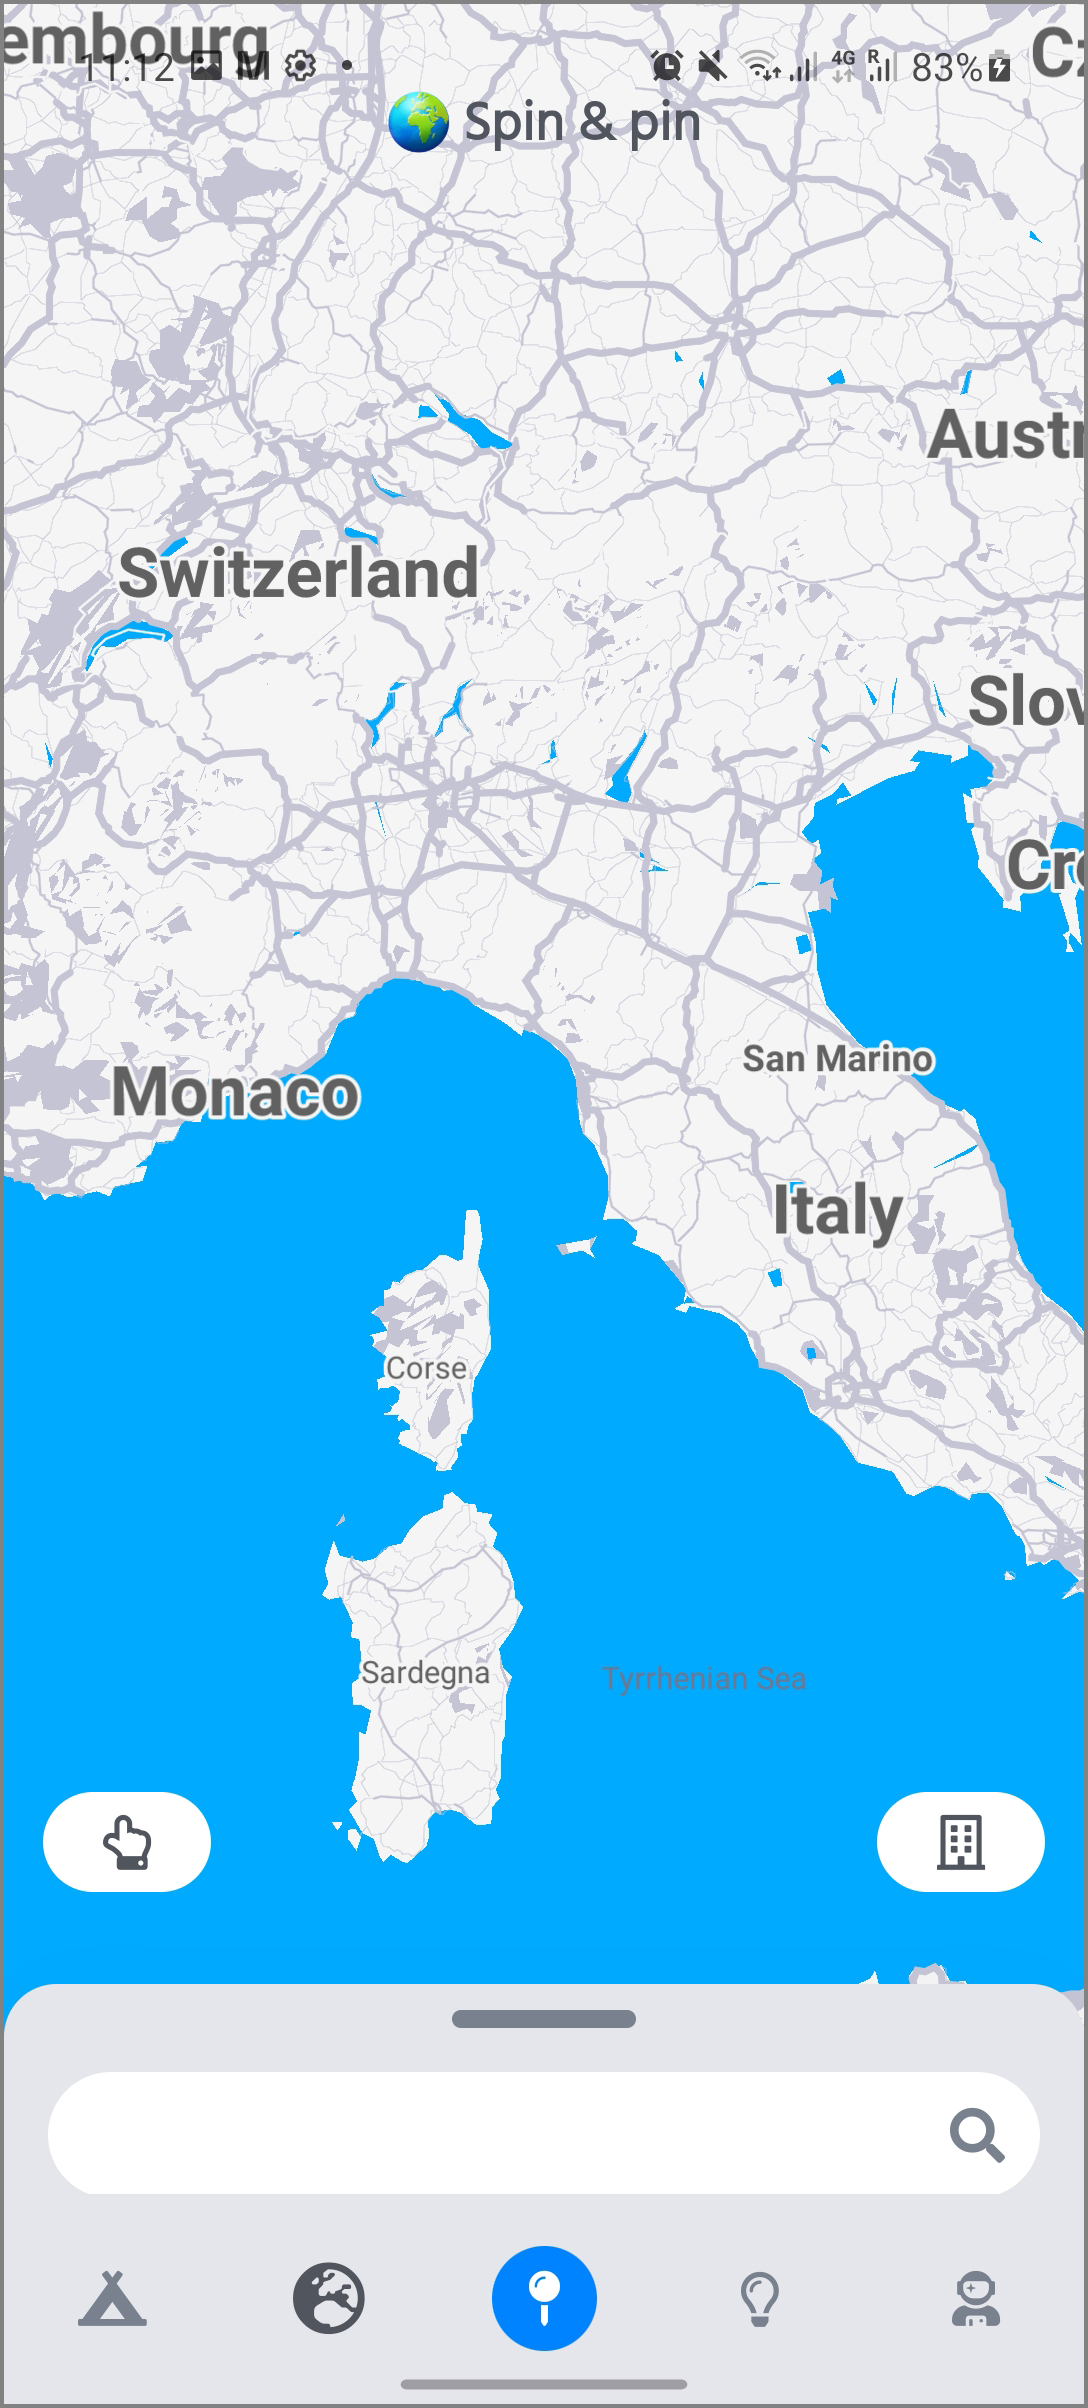
\includegraphics[width=.9\textwidth]{../Images/UI/MapSearchLight.jpg}
\caption{\label{fig:dbapiuser}\textbf{Map screen in light style}}
\end{minipage} 
\begin{minipage}{.48\textwidth}
\centering
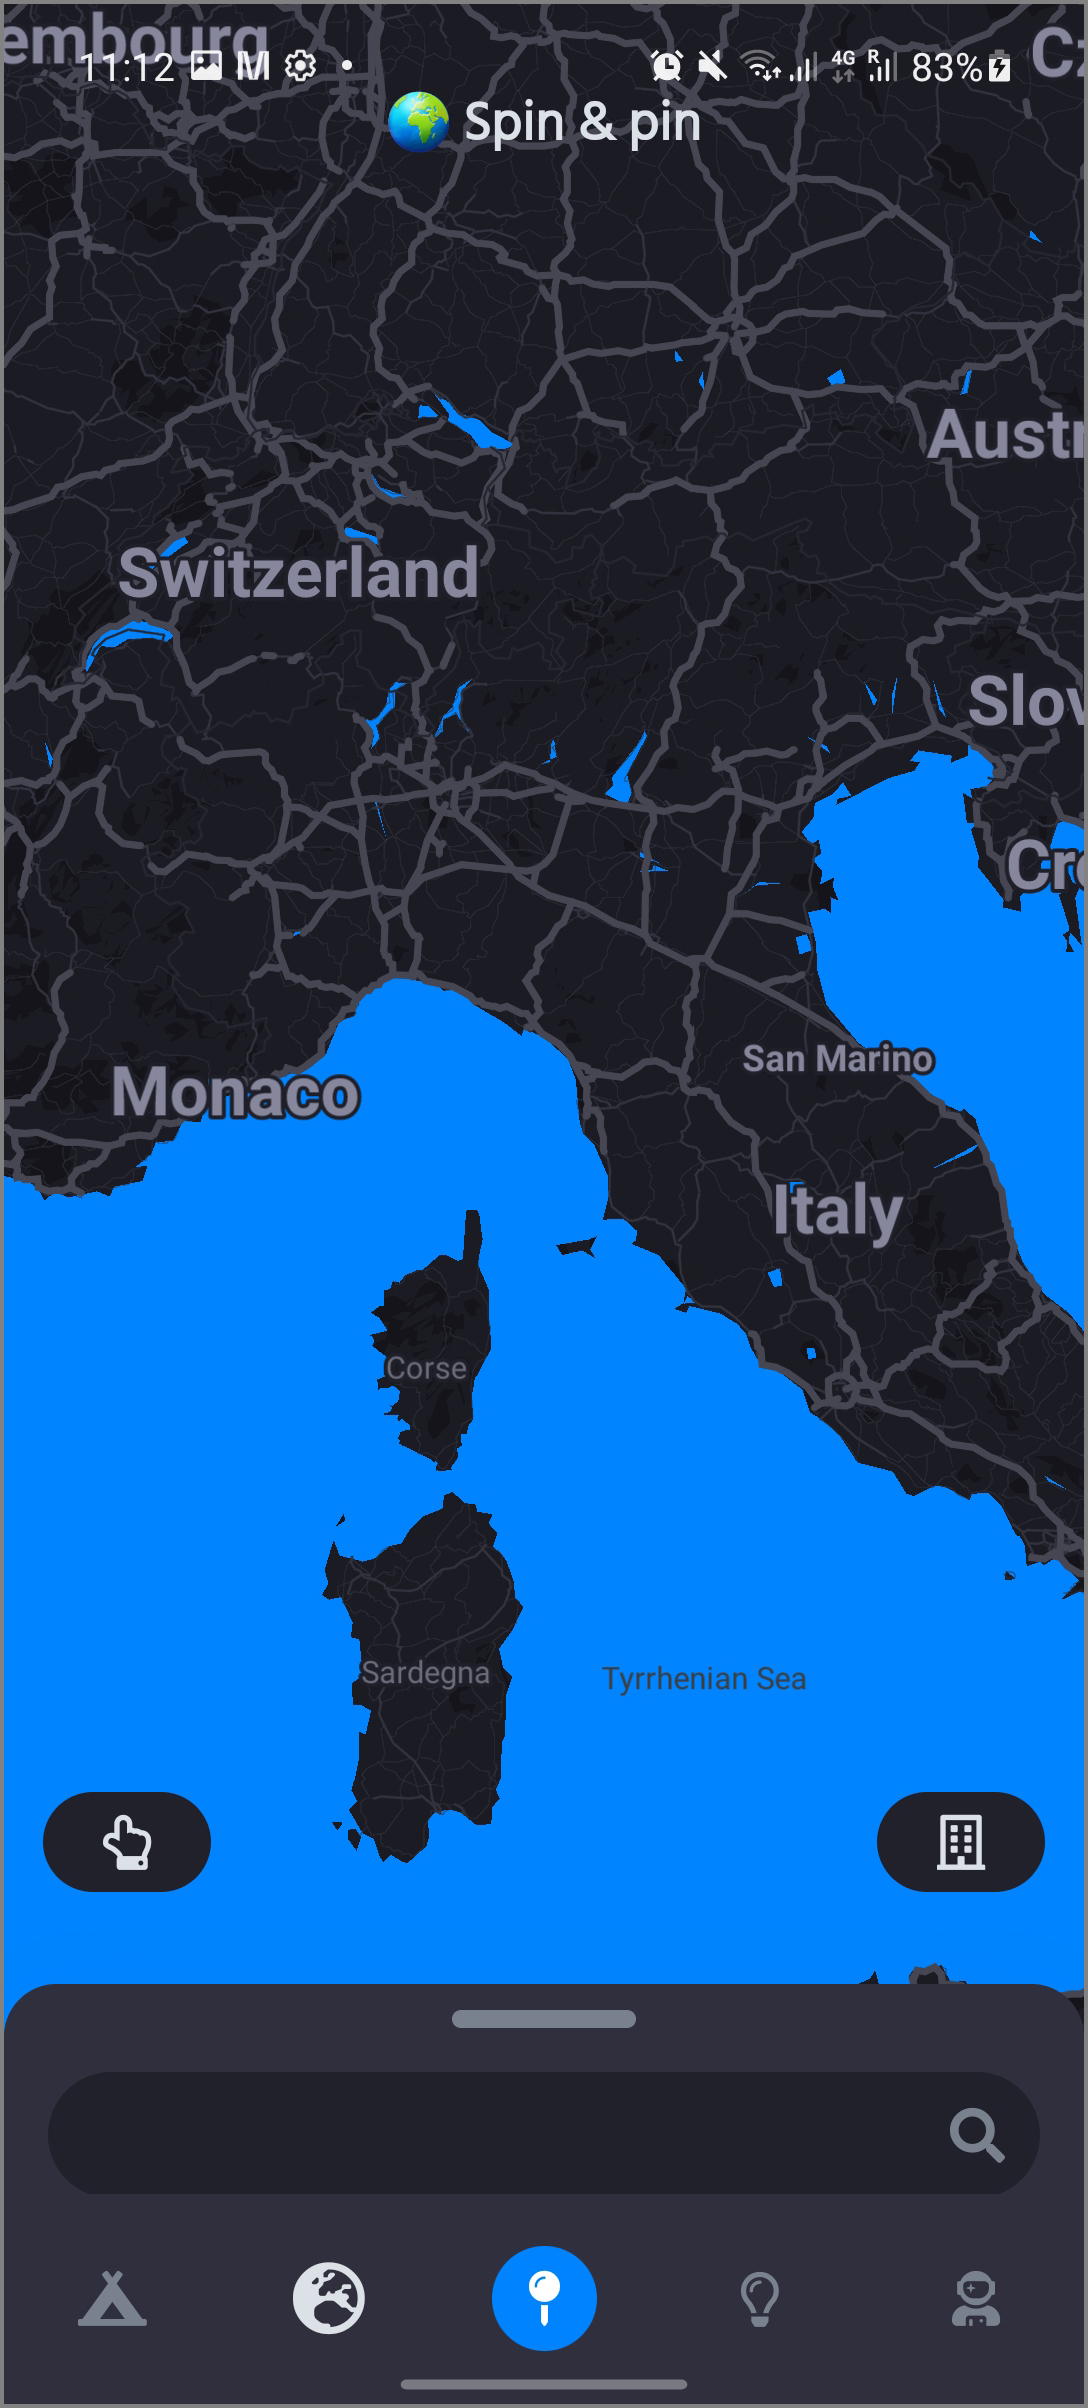
\includegraphics[width=.9\textwidth]{../Images/UI/MapSearchDark.jpg}
\caption{\label{fig:dbapiuser}\textbf{Map screen in dark style}}
\end{minipage}
\end{figure}

Map screen allows users to interactively go through the desired locations on the map and find small icons that represent trips in that area. Map takes into account the boundaries that are shown on the screen and actively adjusts the search parameters, fetching from the database only the trips that are in the current area. Map helps users explore certain areas when they are not sure which specific destination to center their trip around.
\newpage

\subsubsection{Saved trips screen}
\begin{figure}[!htb]
\centering
\begin{minipage}{.48\textwidth}
\centering
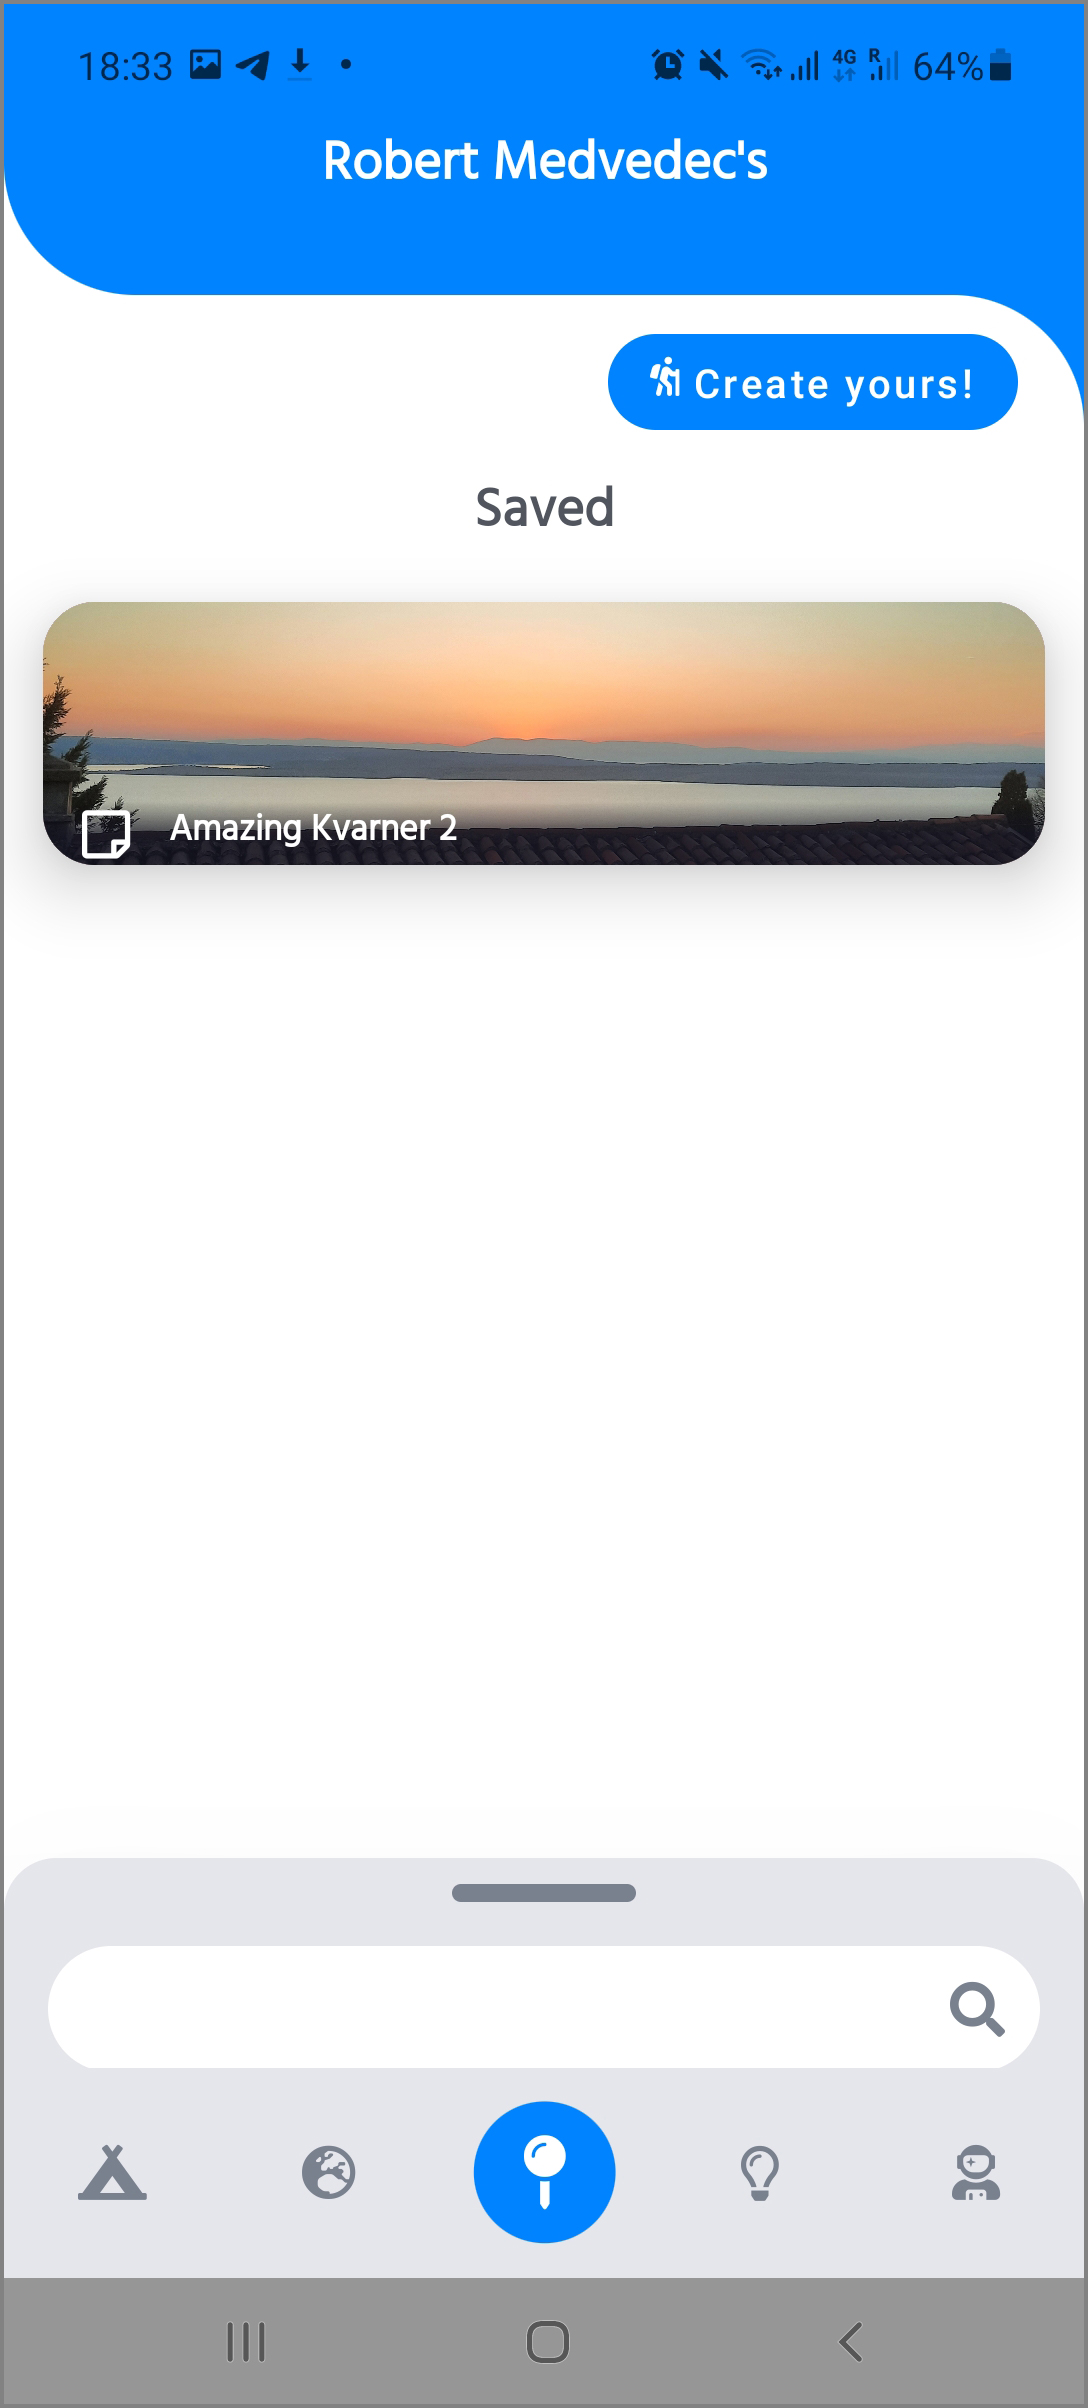
\includegraphics[width=.9\textwidth]{../Images/UI/MyTripsWhite.jpg}
\caption{\label{fig:dbapiuser}\textbf{Saved trips screen in light style}}
\end{minipage} 
\begin{minipage}{.48\textwidth}
\centering
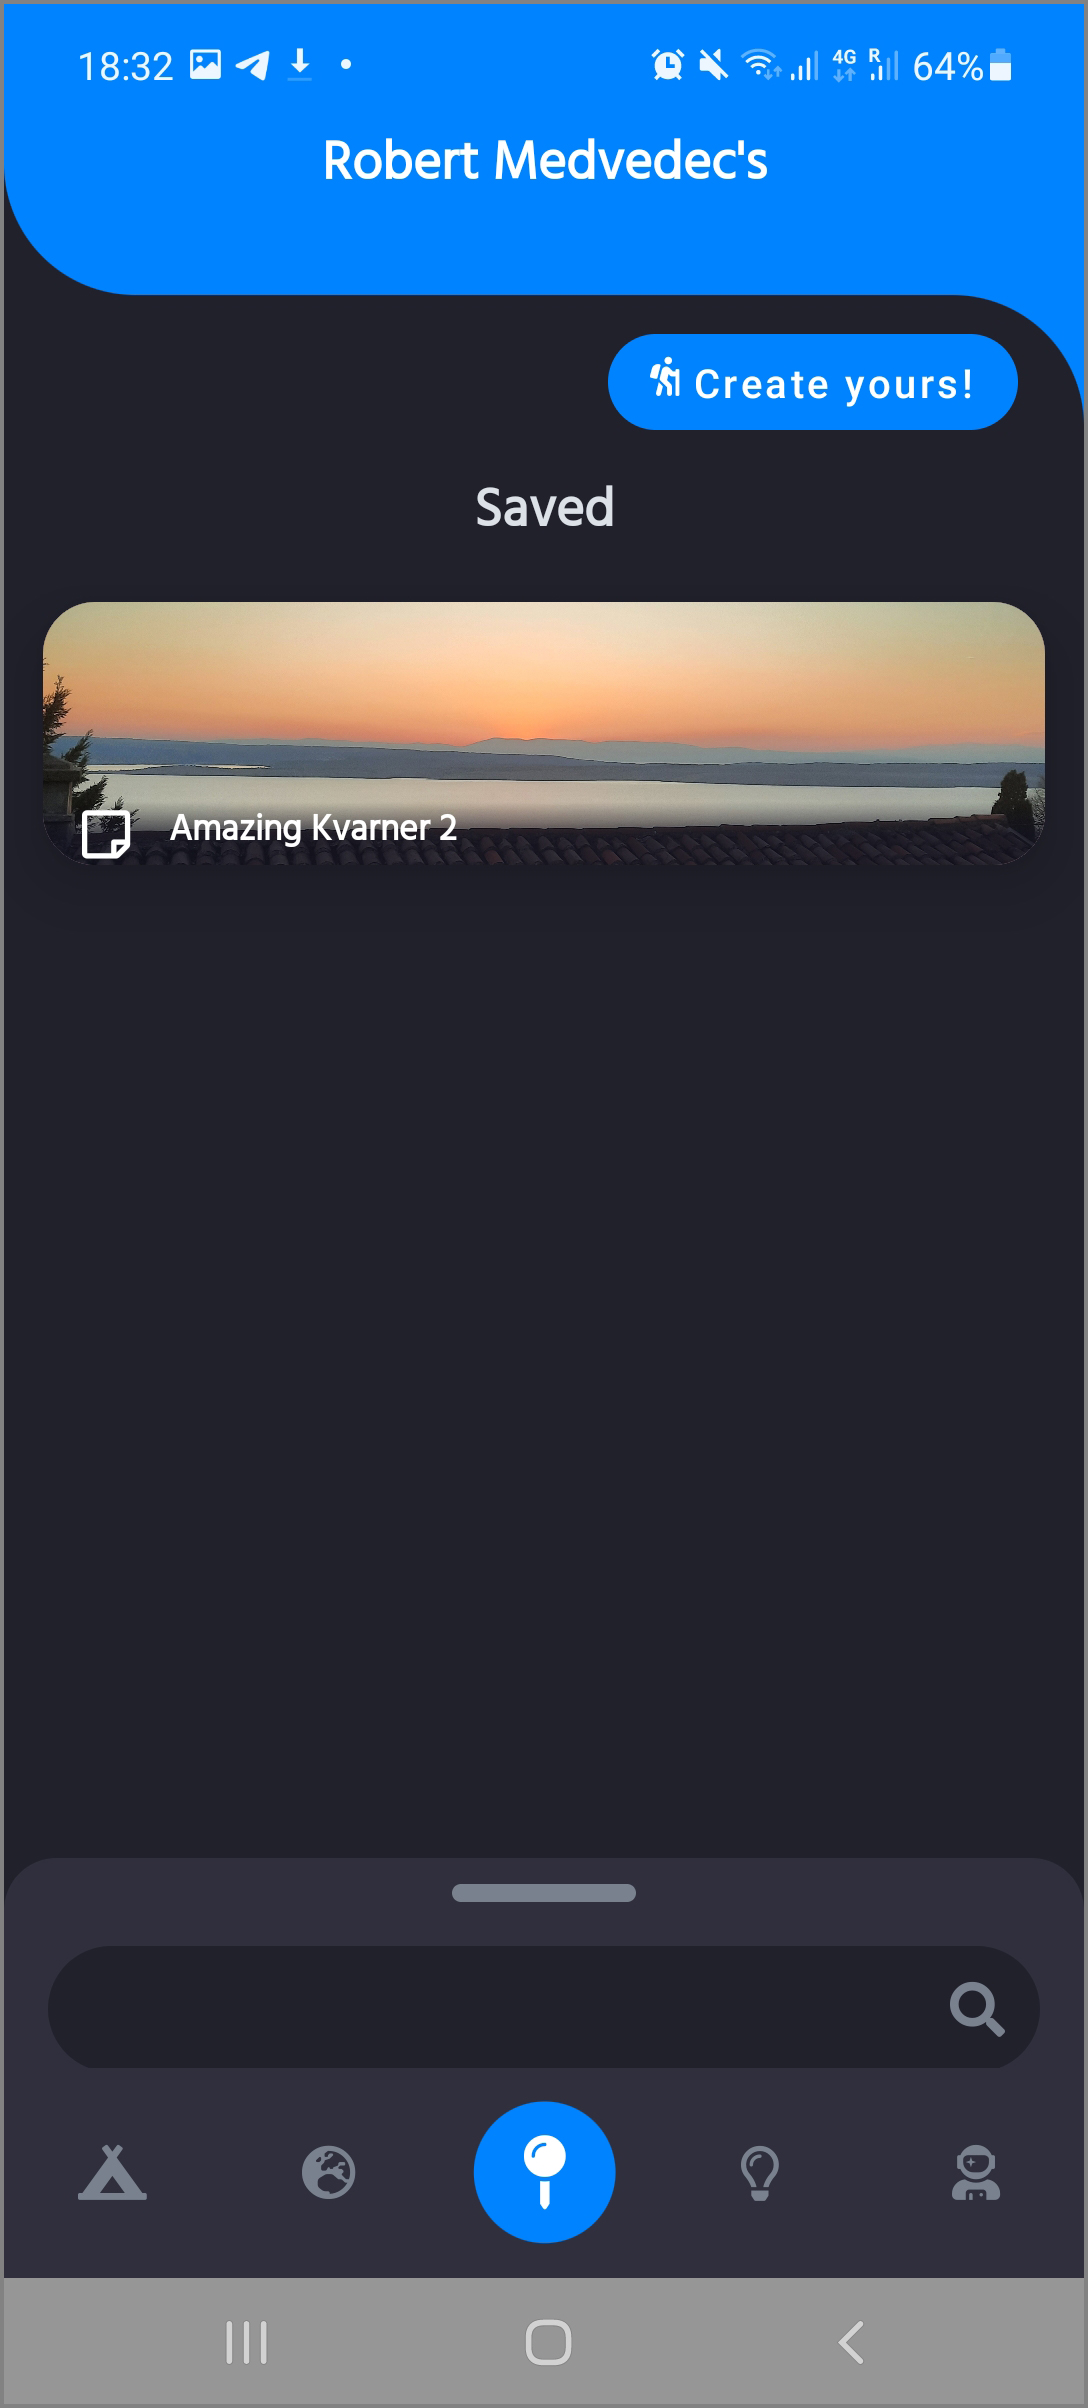
\includegraphics[width=.9\textwidth]{../Images/UI/MyTripsDark.jpg}
\caption{\label{fig:dbapiuser}\textbf{Saved trips screen in dark style}}
\end{minipage}
\end{figure}

Saved trips screen holds the information of all of the trips the user has created or saved. It is also a quick way of finding older trips that users found interesting and allows them to organize their travels in an easy and effective way.
 
\newpage
\subsubsection{Explore screen}
\begin{figure}[!htb]
\centering
\begin{minipage}{.48\textwidth}
\centering
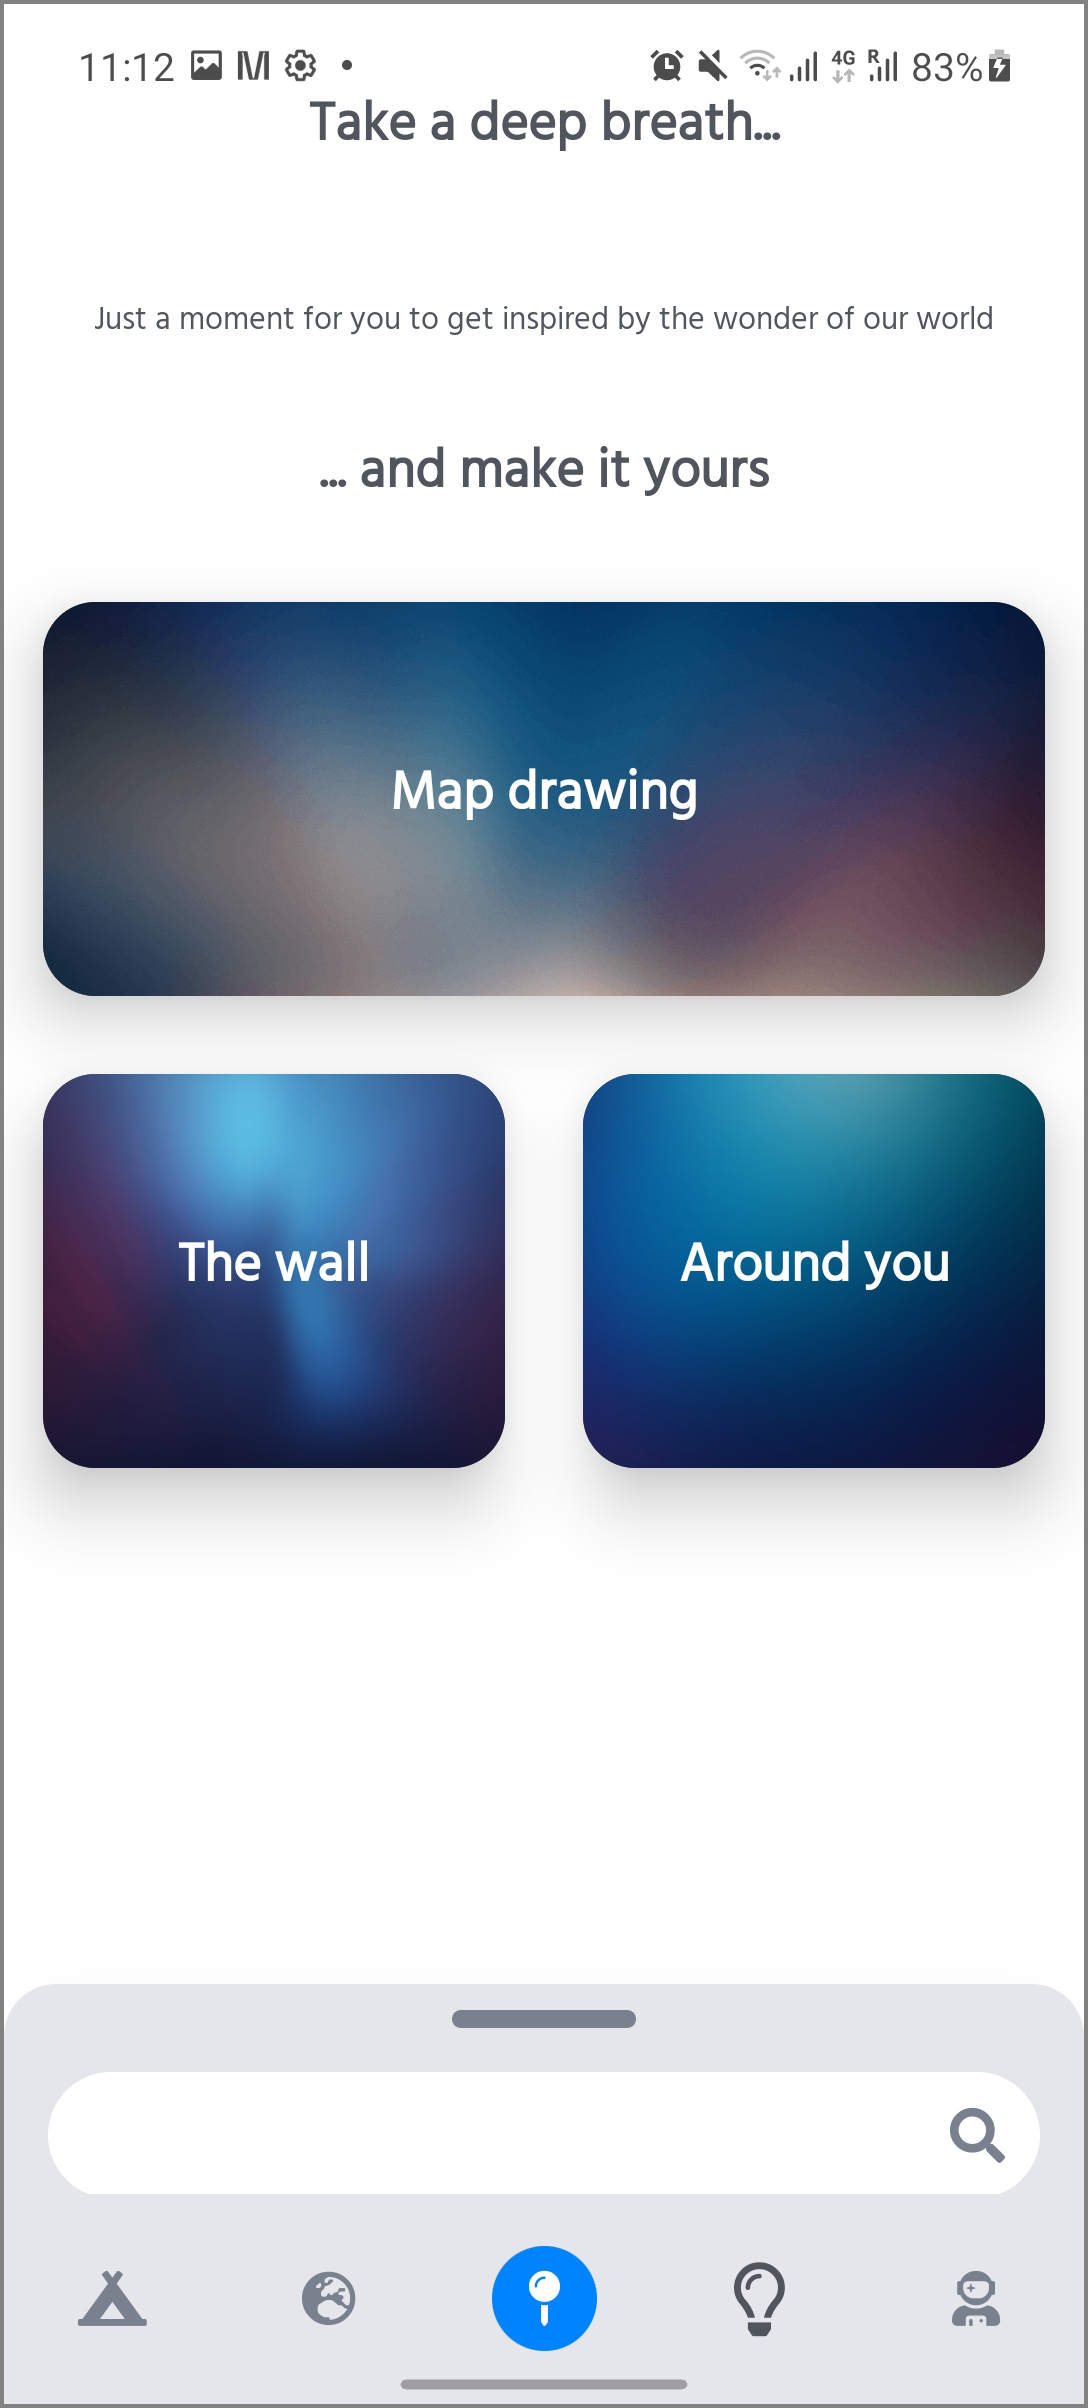
\includegraphics[width=.9\textwidth]{../Images/UI/ExploreLight.jpg}
\caption{\label{fig:dbapiuser}\textbf{Explore screen in light style}}
\end{minipage} 
\begin{minipage}{.48\textwidth}
\centering
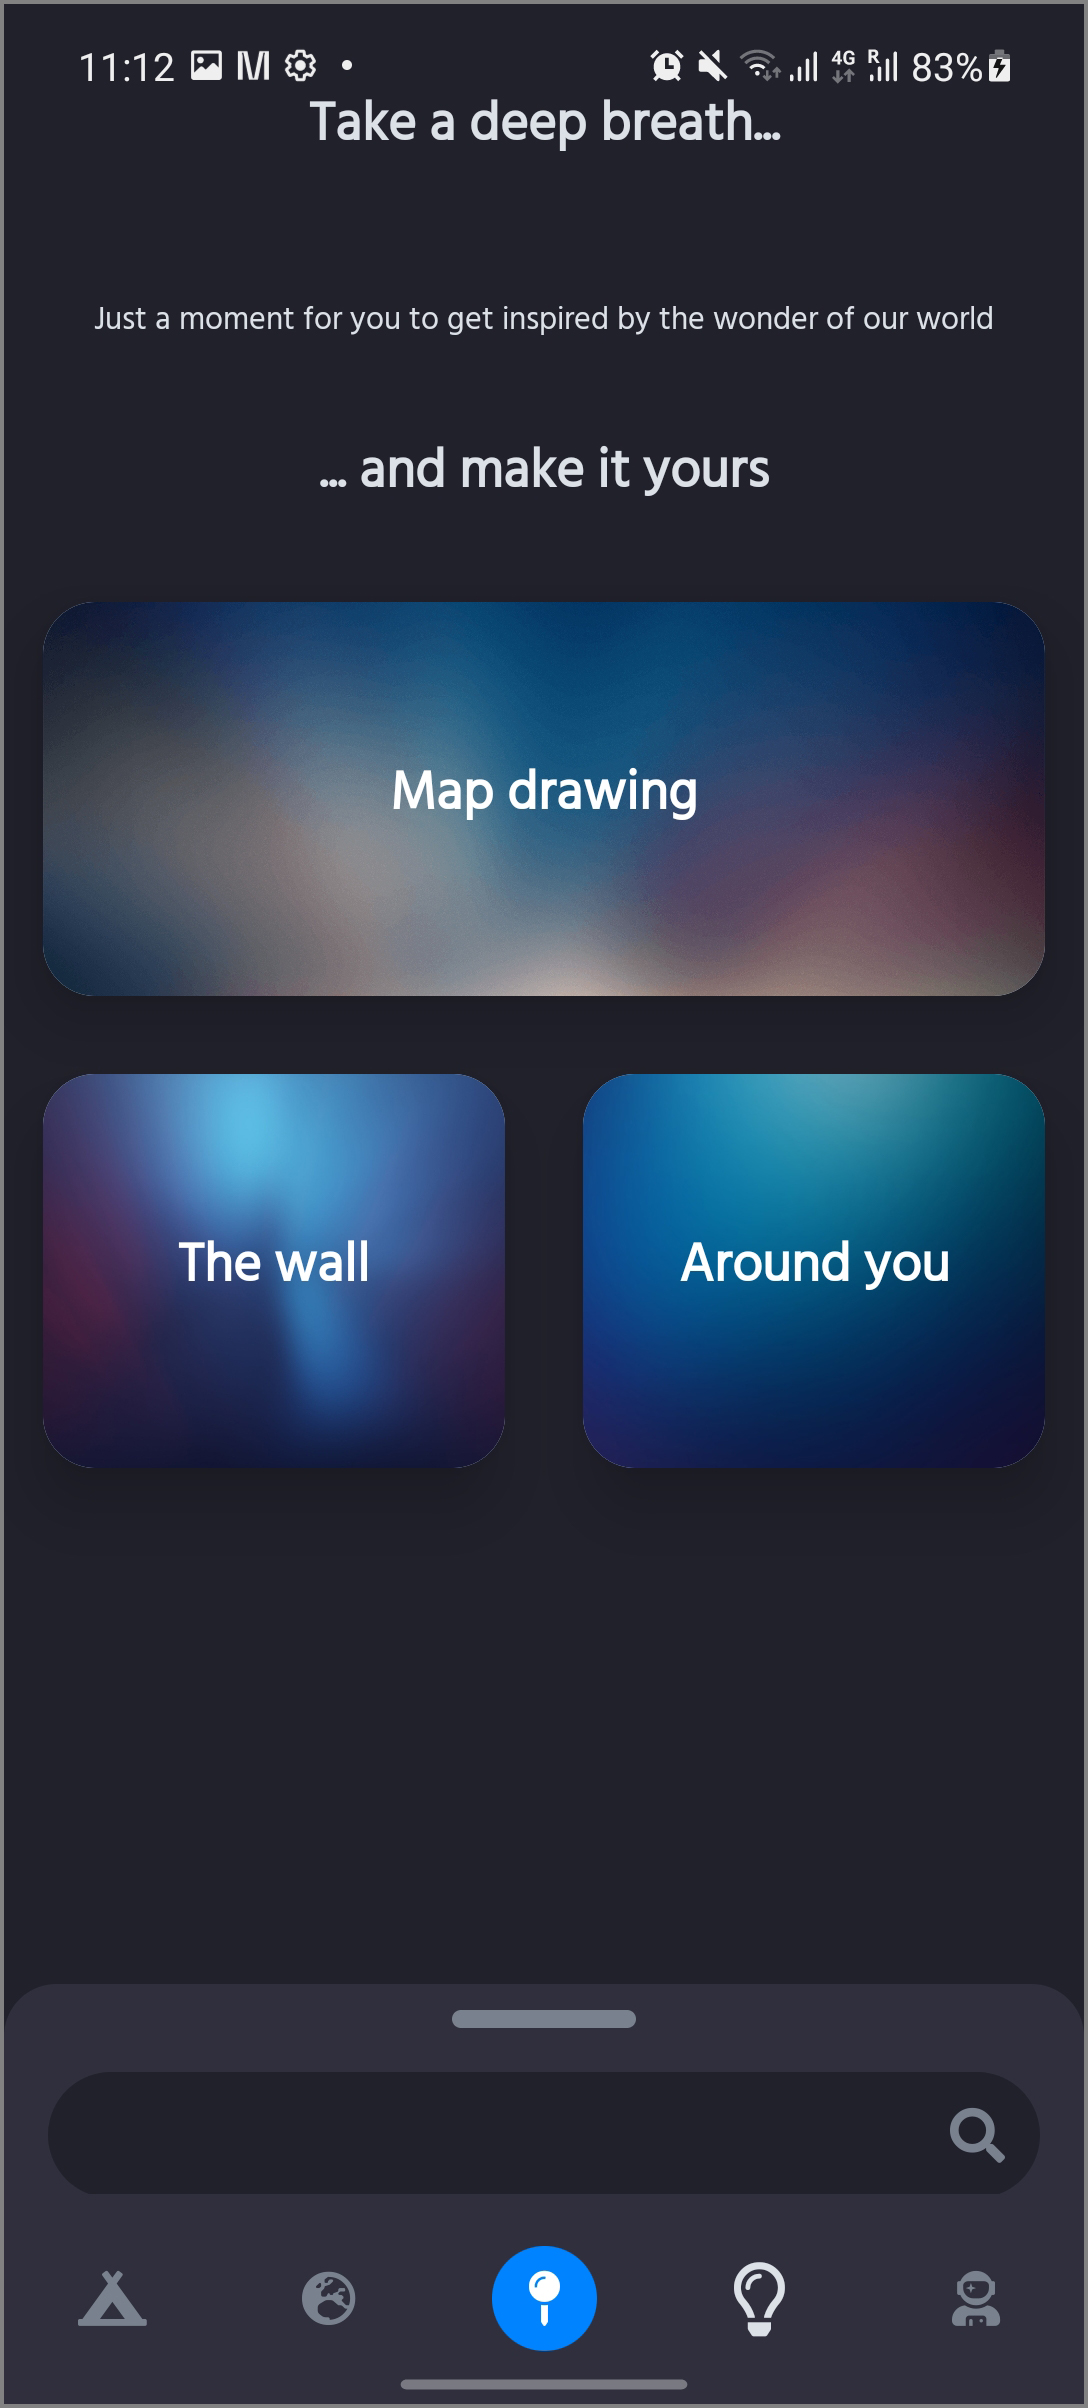
\includegraphics[width=.9\textwidth]{../Images/UI/ExploreDark.jpg}
\caption{\label{fig:dbapiuser}\textbf{Explore screen in dark style}}
\end{minipage}
\end{figure}

Explore screen allows users to search for their future trips in multiple ways. The first way is by searching on the map, and by clicking the 'Map drawing' button, the app takes the user to the previously explained screen.\\ \\
The next option, 'The wall',  - DOESN?T DO ANYTHING NOW. \\ \\
Finally, 'Around you' button asks the user for location permission, and if granted, searches for interesting destinations and trips in the user's vicinity.
 
\newpage
\subsubsection{Settings screen}
\begin{figure}[!htb]
\centering
\begin{minipage}{.48\textwidth}
\centering
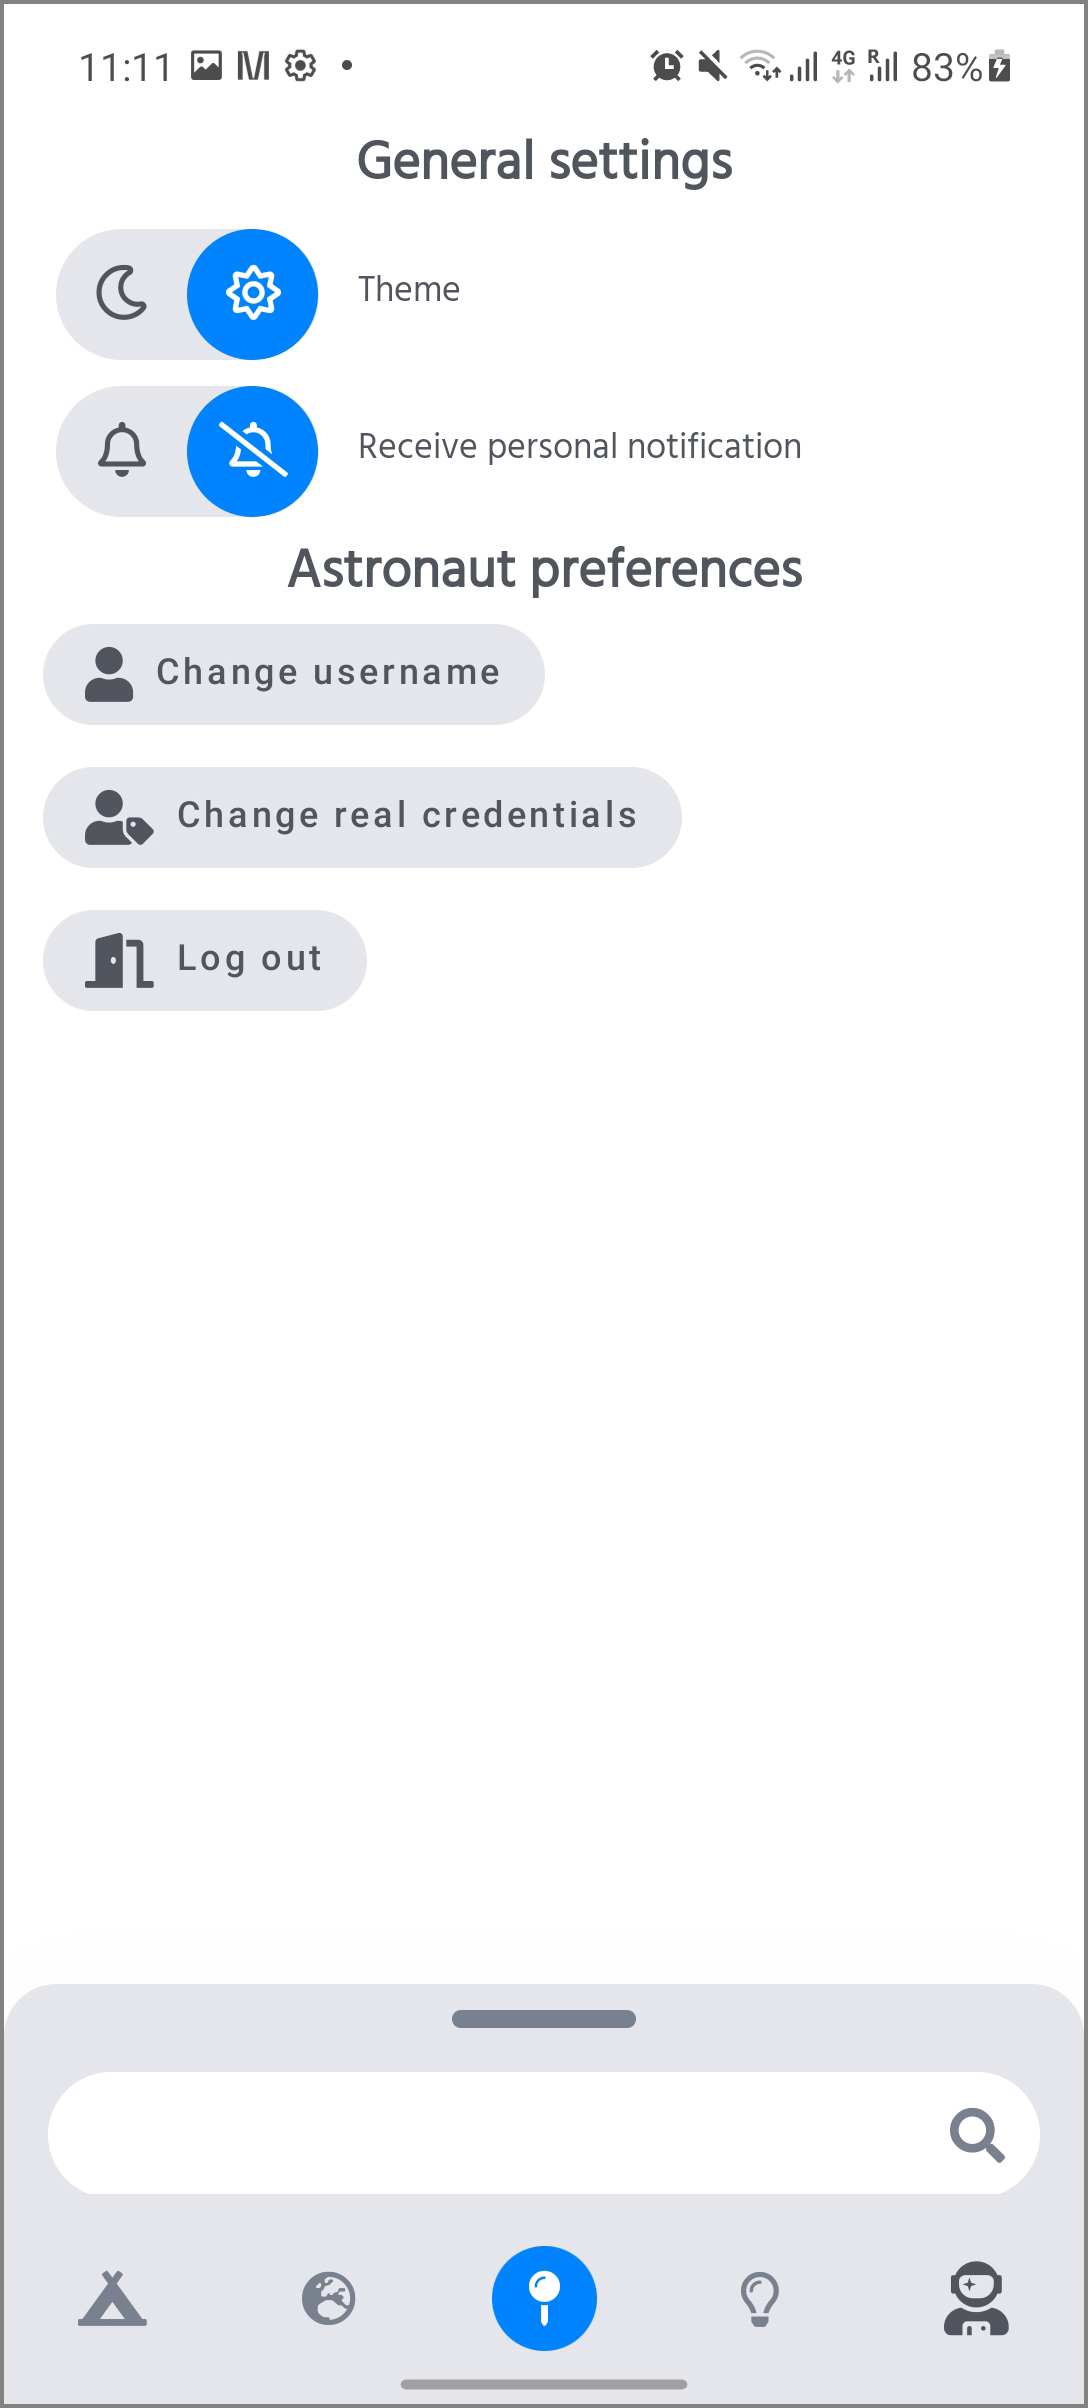
\includegraphics[width=.9\textwidth]{../Images/UI/SettingsLight.jpg}
\caption{\label{fig:dbapiuser}\textbf{Settings screen in light style}}
\end{minipage} 
\begin{minipage}{.48\textwidth}
\centering
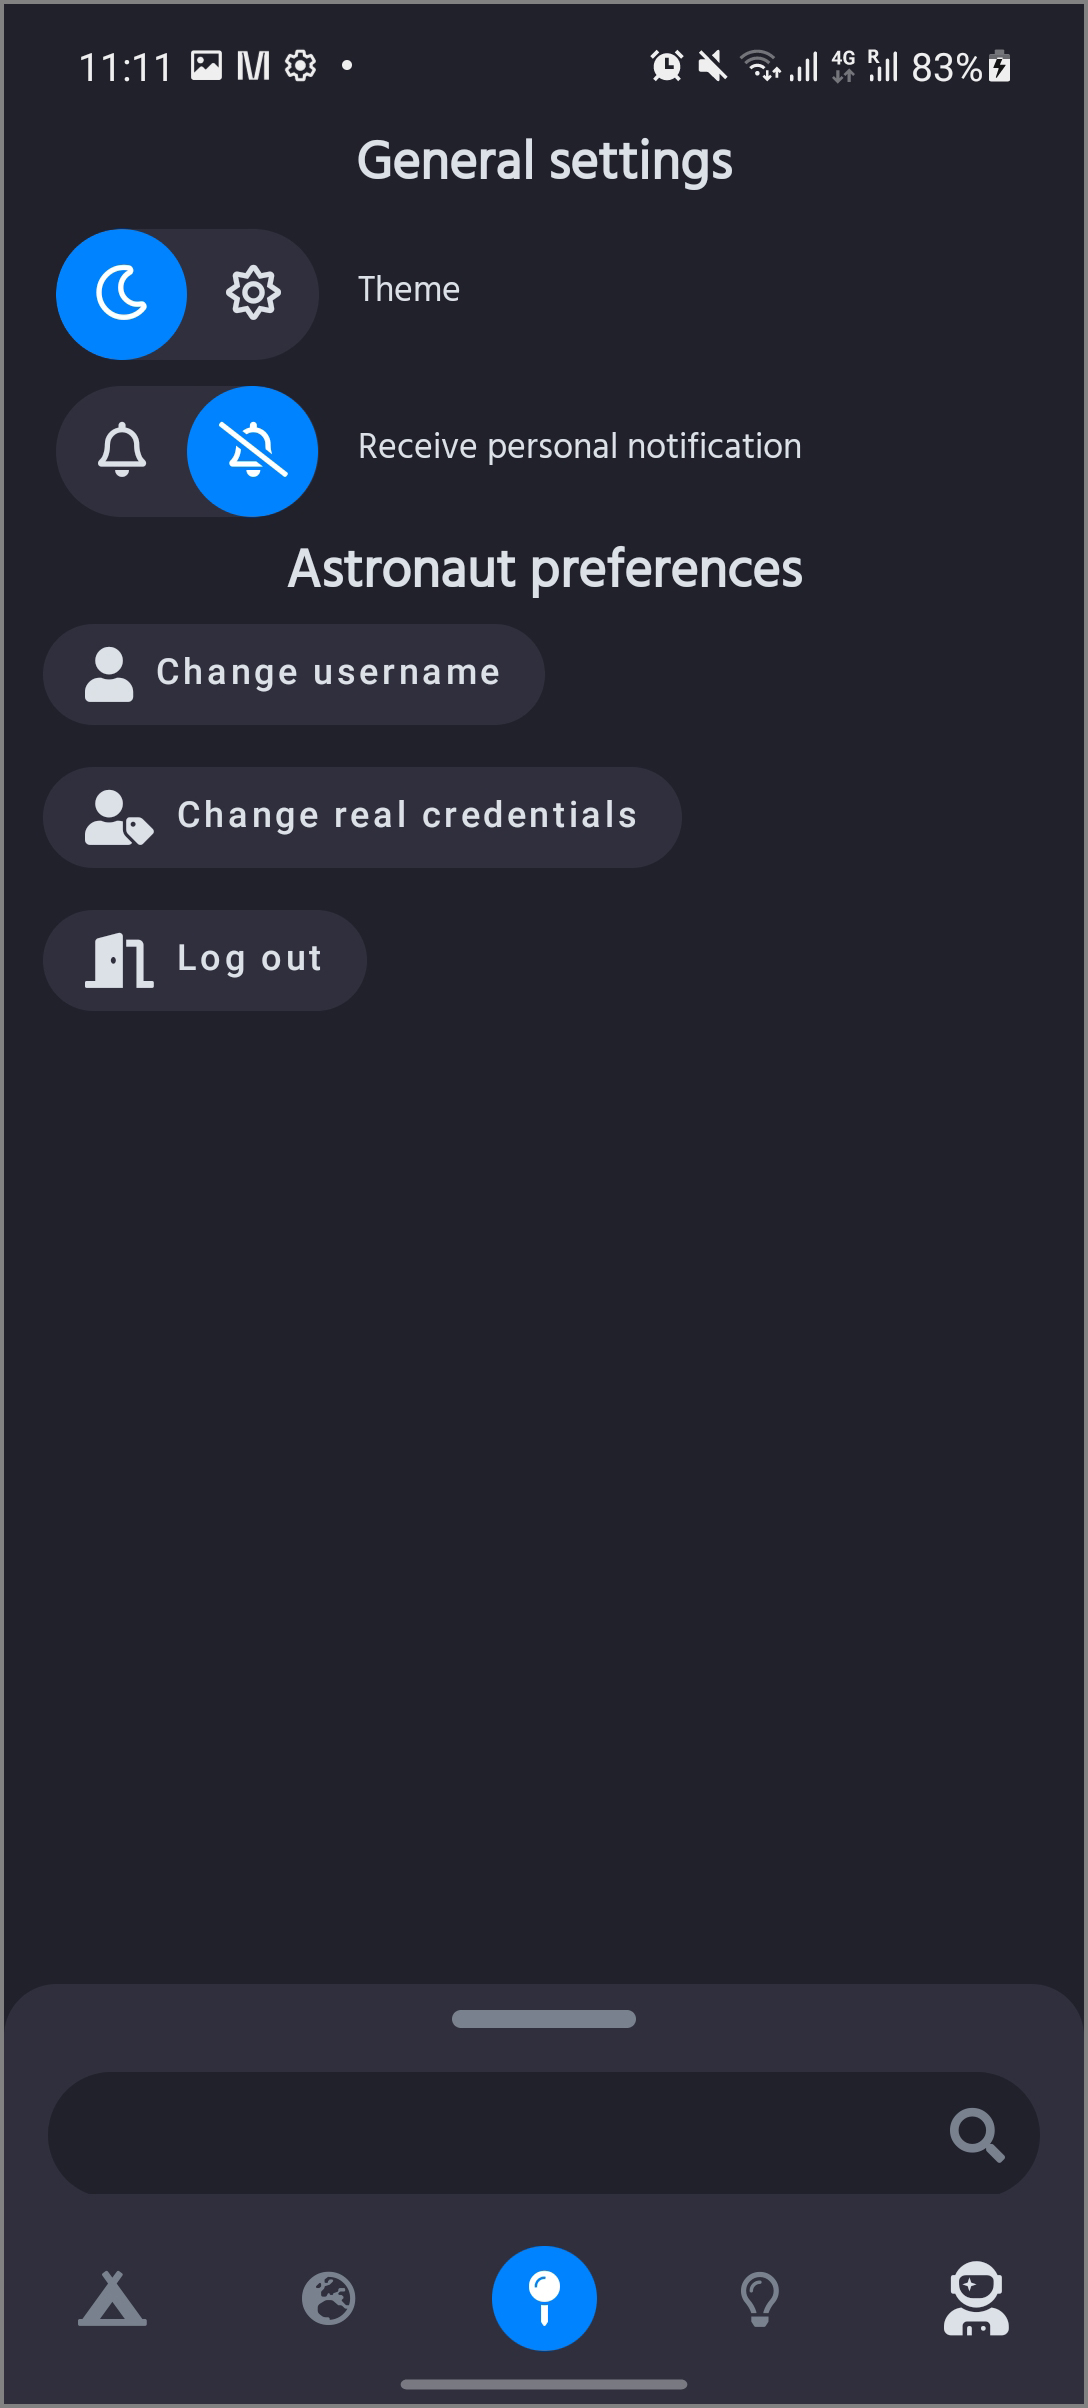
\includegraphics[width=.9\textwidth]{../Images/UI/SettingsDark.jpg}
\caption{\label{fig:dbapiuser}\textbf{Settings screen in dark style}}
\end{minipage}
\end{figure}

Settings screen allows users to change between dark and light theme, to turn the notifications on or off, and to change user preferences such as username and real credentials, which are optional. It also features an option to log out, if user ever wishes to change their account. 
 
\newpage
\subsubsection{Trip creation screen}
\begin{figure}[!htb]
\centering
\begin{minipage}{.48\textwidth}
\centering
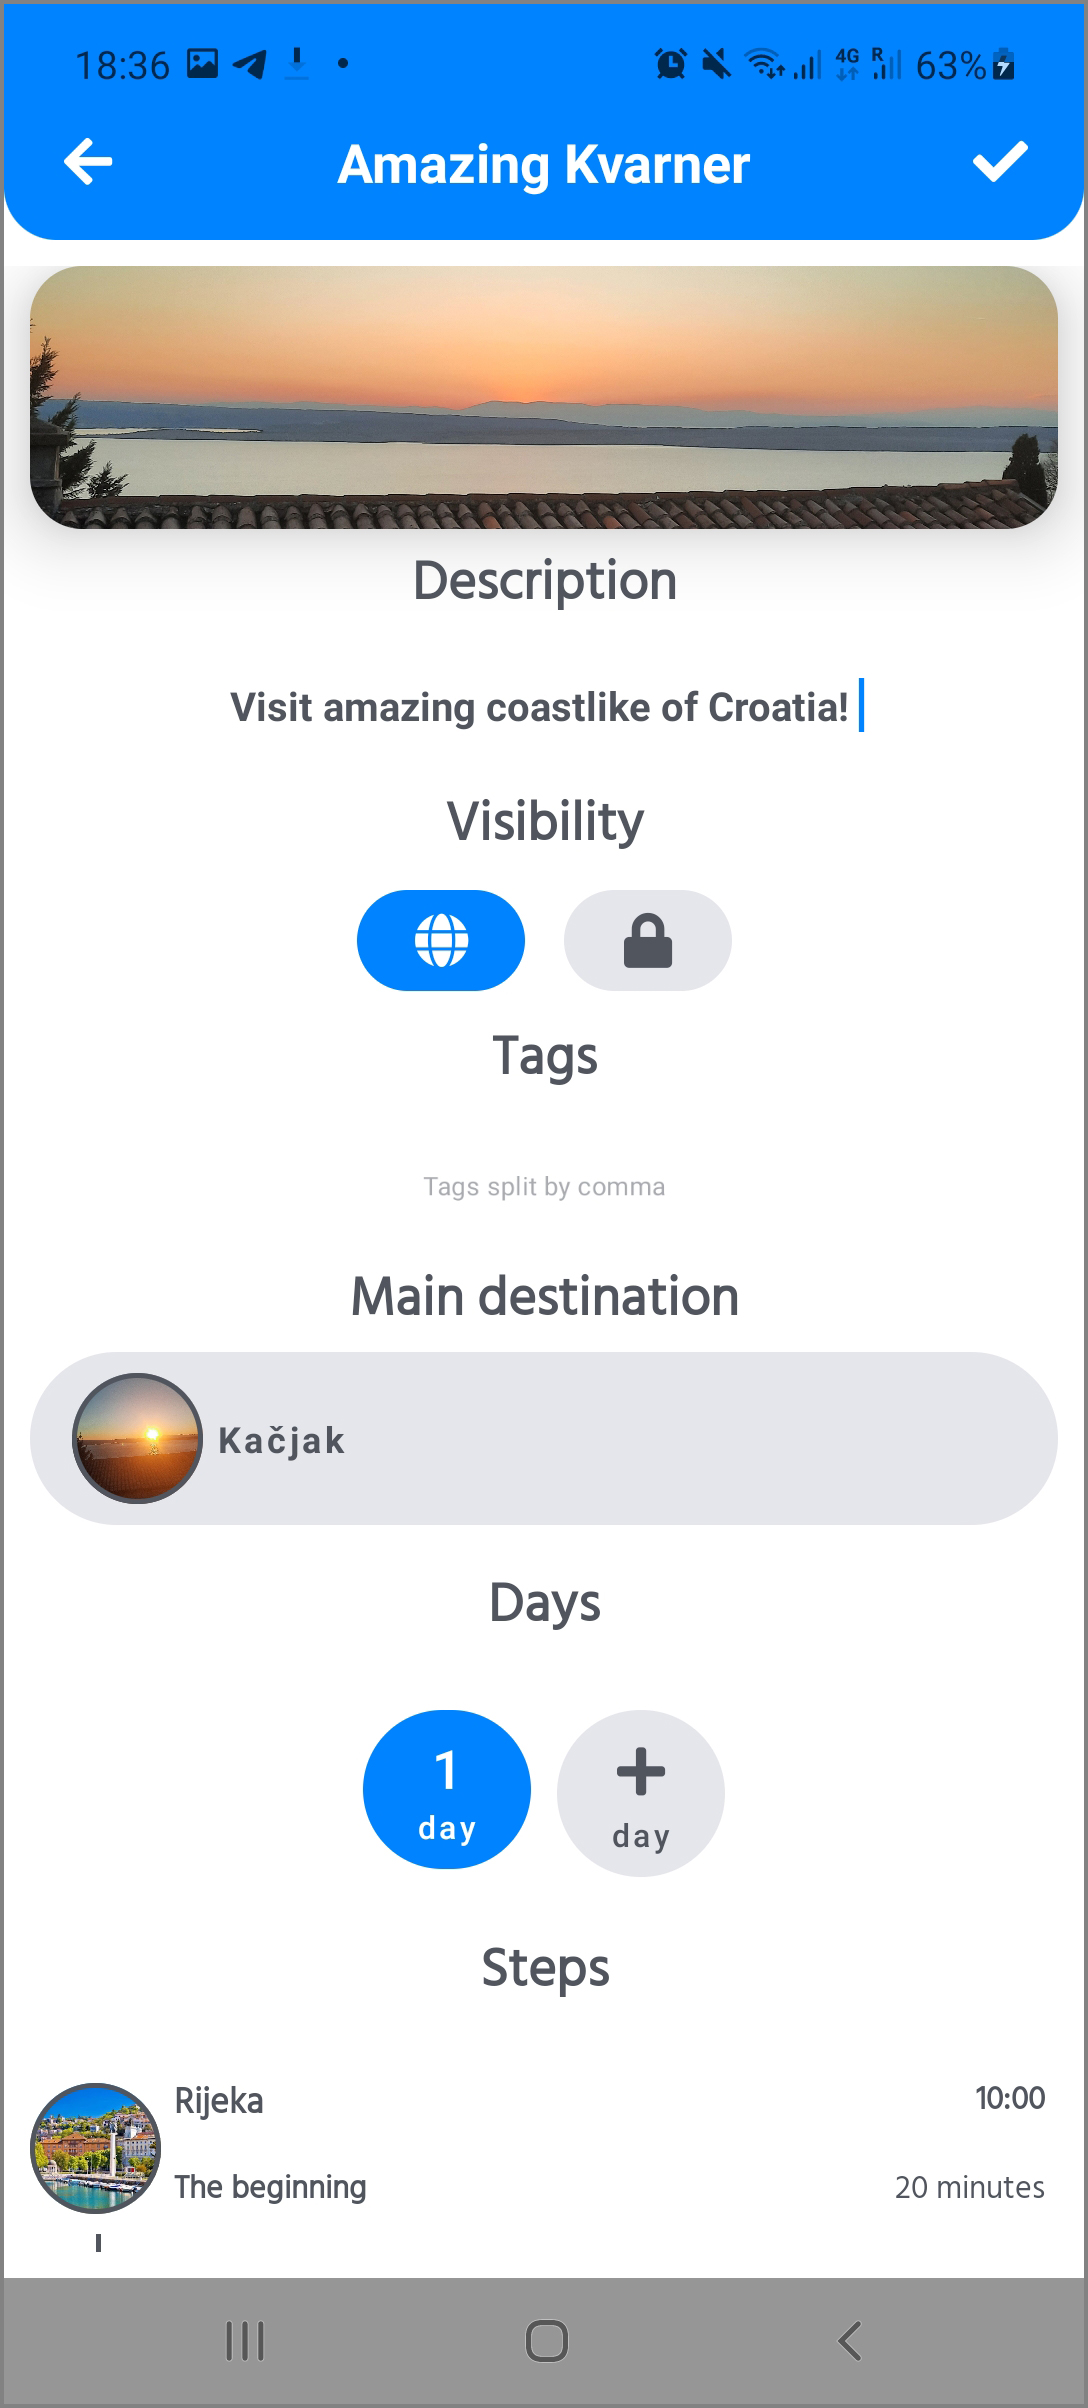
\includegraphics[width=.9\textwidth]{../Images/UI/TripCreateWhite.jpg}
\caption{\label{fig:dbapiuser}\textbf{Trip creation screen in light style}}
\end{minipage} 
\begin{minipage}{.48\textwidth}
\centering
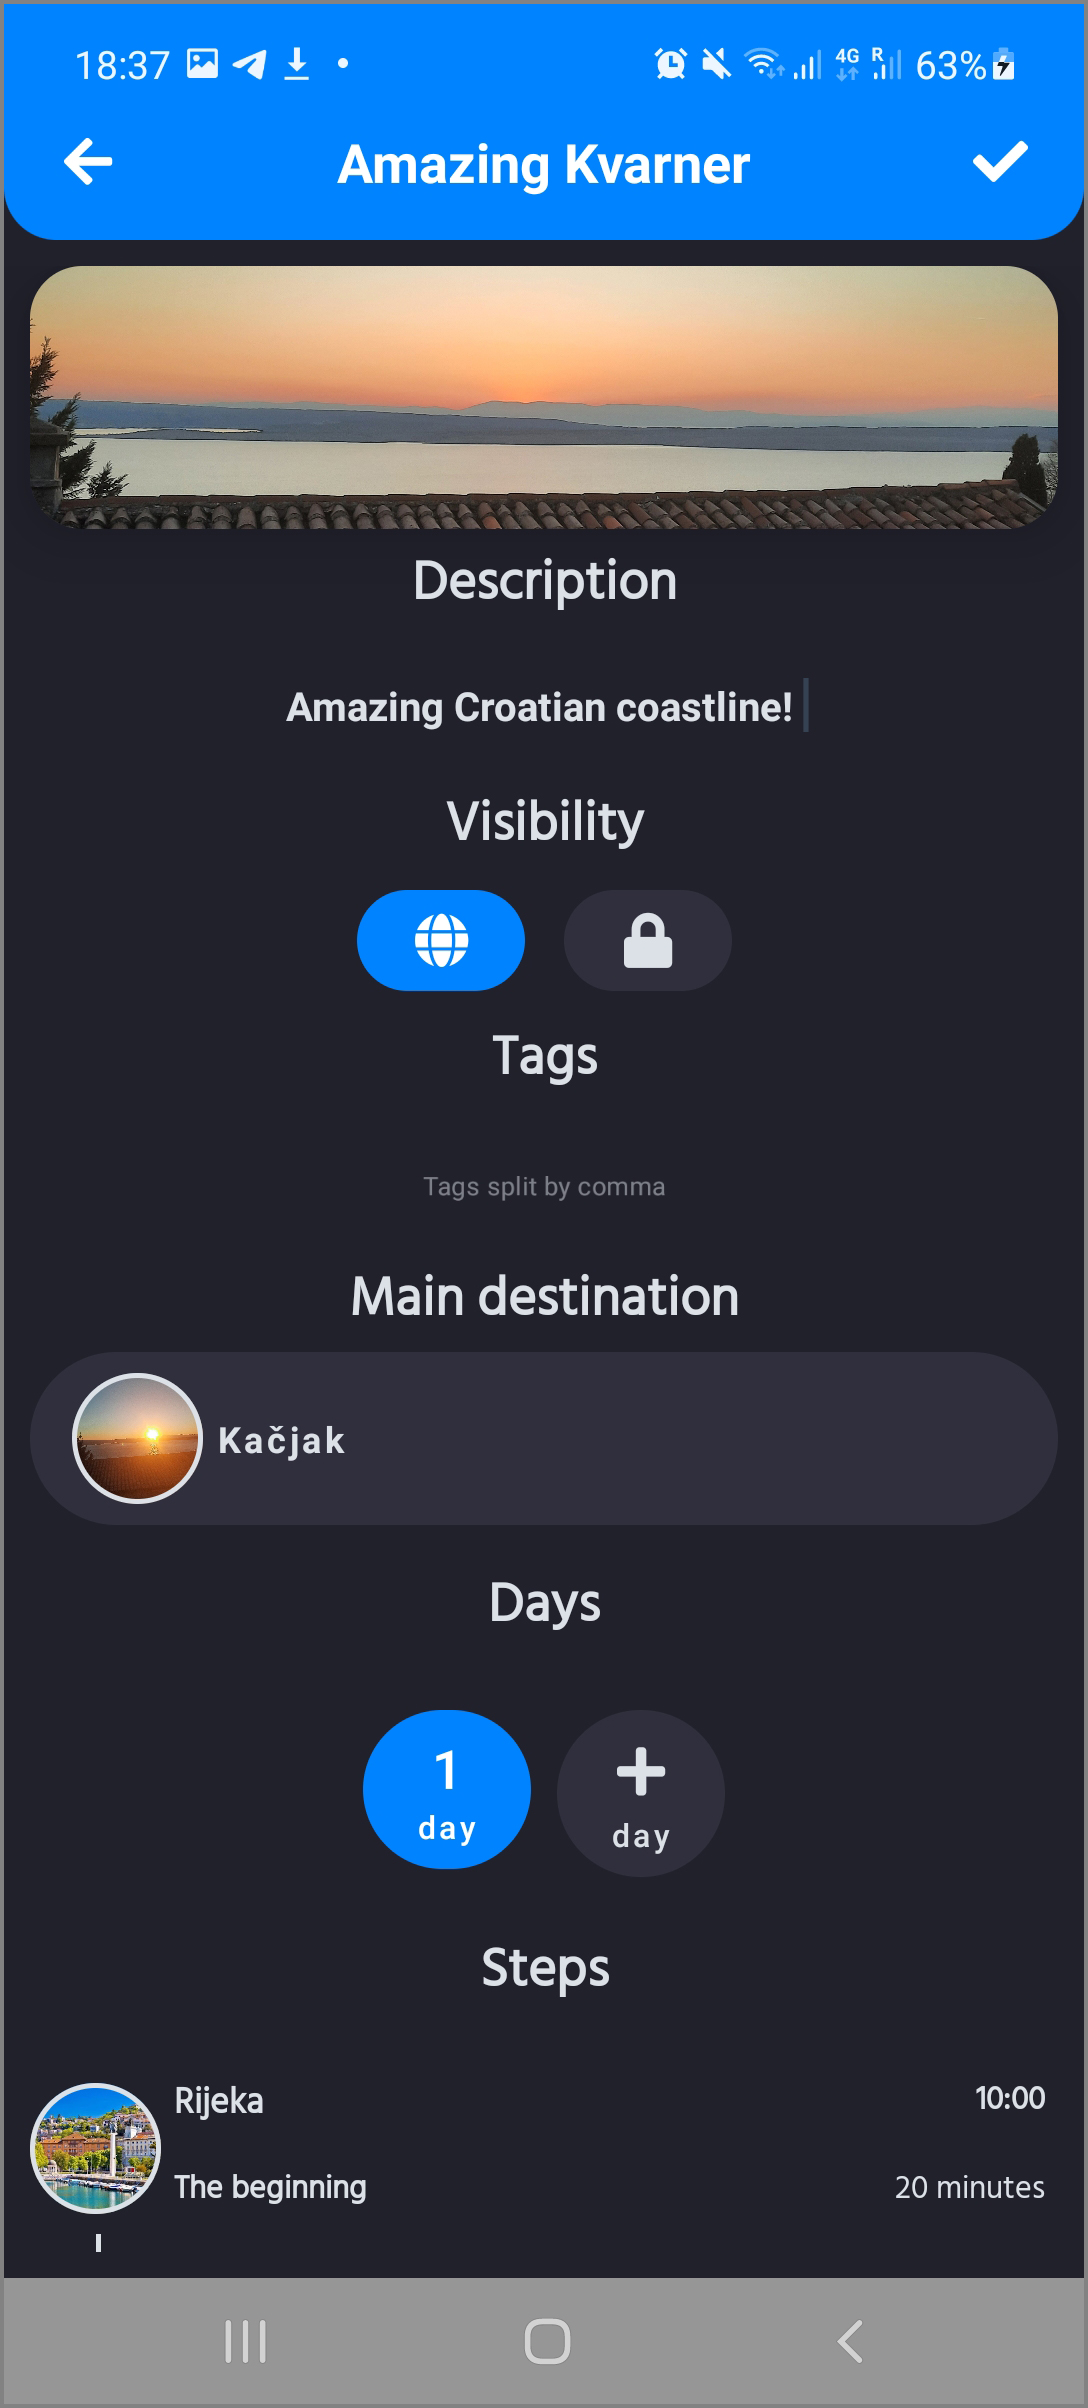
\includegraphics[width=.9\textwidth]{../Images/UI/TripCreateDark.jpg}
\caption{\label{fig:dbapiuser}\textbf{Trip creation screen in dark style}}
\end{minipage}
\end{figure}

This is the way the trip creation looks like, with its functionality previously explained in the document. This screen also features several sub screens, which are not presented in the document due to conciseness.


%------------------------------------------------------------------------------------------------------------------------------------------------
\clearpage
{\color{Blue}{\section{Testing}}}
\label{sect:test}
\hspace{\parindent}Several test types have been done for the app. Most of the testing was done during the app development, so further Unit testing was reduced as most of it was done before.

\subsection{Unit testing}
\hspace{\parindent}The main part of the testing was done by unit testing.
Four major unit tests have been created that test functionalities of the main parts of the app. Each main test has several subtests. For code conciseness purposes main tests are not a set of small tests, but just one large test that tests multiple different parts of the subsystem.\\ \\

When counting the total number of tested subcomponents, we have done approximately XY small tests, separated into four major groups, which are:
\begin{itemize}
\item Login tests (7)
\item Trip Creation Activity tests (12)
\item Navigation tests (6)
\item Map screen tests (5)
\end{itemize}

These tests are now going to be showcased and presented.
\subsubsection{Login unit testing}
The tests done for login testing:
\begin{itemize}
\item Inputting username
\item Inputting password
\item Testing login
\item Testing login with false authentication
\item Testing login with correct authentication
\item Logging in with Google Account
\item Logging in with Facebook acocunt
\end{itemize}

The code:
\begin{verbatim}
@RunWith(AndroidJUnit4::class)
class LoginTest : TestCase() {

    @OptIn(
        ExperimentalFoundationApi::class,
    kotlinx.coroutines.ExperimentalCoroutinesApi::class,
        androidx.compose.animation.ExperimentalAnimationApi::class,
        androidx.compose.material.ExperimentalMaterialApi::class
    )
    @get:Rule
    val composeTestRule = createAndroidComposeRule<LoginActivity>()
    @OptIn(
        ExperimentalCoroutinesApi::class,
        androidx.compose.foundation.ExperimentalFoundationApi::class,
        androidx.compose.animation.ExperimentalAnimationApi::class,
        androidx.compose.material.ExperimentalMaterialApi::class
    )
    @Test
    fun checkLogin() {
        val login = composeTestRule.onNodeWithTag("login")
        val usr = composeTestRule.onNodeWithTag("username")
        val pwd = composeTestRule.onNodeWithTag("password")
            usr.performTextInput("vins@vins.com")
            pwd.performTextInput("vins")
            login.performClick()
        composeTestRule.onNode(hasText("Authentication failed"))
        assertFalse(composeTestRule.activity.isNewUser ?: false)
        pwd.performTextClearance()
        pwd.performTextInput("vinsvins")
        login.performClick()
        Thread.sleep(5000)
        getInstrumentation().runOnMainSync {
            val activity =
                ActivityLifecycleMonitorRegistry.getInstance().getActivitiesInStage(
                    Stage.RESUMED
                ).first()
            assertTrue(activity is MainActivity)
        }
    }
}

\end{verbatim}

\subsubsection{Trip creation activity unit testing}
The tests done for trip creation activity testing:
\begin{itemize}
\item Tests whether the trip can be created correctly.
\item The following elements of the trip creation screen are tested:
\item Inputting text to name field
\item Inputting text to description field
\item Inputting multiple tags
\item Searchig destinations with city name
\item Adding steps
\item Adding main destinations
\item Exiting without saving
\item Exiting with saving
\item Trying to save trip without filling all the required fields
\item Failing to save trip
\end{itemize}

\begin{verbatim}
-	@RunWith(AndroidJUnit4::class)
class TripCreationActivityTest : TestCase() {
    @get:Rule
    val composeTestRule = createAndroidComposeRule<TripCreationActivity>()
    @OptIn(ExperimentalTestApi::class)
    @Test
    fun create() {
        composeTestRule.onNodeWithTag("name").performTextInput("Nome")
        composeTestRule.onNodeWithTag("description").
        performTextInput("Description")
        val tag = composeTestRule.onNodeWithTag("tag")
        tag.performTextInput("tag1")
        tag.performTextInput(",")
        tag.performTextInput("tag2")
        tag.performTextInput(",")
        composeTestRule.onNodeWithTag("main").performClick()
        Thread.sleep(1000)
        composeTestRule.onNodeWithTag("searchText").
        performTextInput("verona")
        composeTestRule.onNodeWithTag("searchText").
        performImeAction()
        Thread.sleep(4000)
        composeTestRule.
        onAllNodes(hasText("Verona",true,true)).
        onFirst().assertExists()
        val addStep = composeTestRule.onAllNodesWithTag("add").onFirst()
        addStep.assertExists()
        addStep.performClick()
        val setMain = composeTestRule.onAllNodesWithTag("main").onFirst()
        setMain.assertExists()
        setMain.performClick()
        composeTestRule.onNodeWithTag("back").performClick()
        Thread.sleep(500)
        val nodes = composeTestRule.onAllNodes(hasText("verona",true,true))
        assertNotNull(nodes)
        nodes.assertCountEquals(2)
        composeTestRule.onNodeWithTag("confirm").performClick()
        Thread.sleep(2000)
        InstrumentationRegistry.getInstrumentation().runOnMainSync {
            val activity =
                ActivityLifecycleMonitorRegistry.getInstance().
            getActivitiesInStage(
                    Stage.DESTROYED
                ).first()

            assertTrue(activity is TripCreationActivity)

        }
    }
    
    @Test
    fun creationFailure() {
        for (i in 0..3) {
            if (i == 0)
                composeTestRule.onNodeWithTag("name").
            performTextInput("Nome")
            if (i == 1)
                composeTestRule.onNodeWithTag("description")
            .performTextInput("Description")
            if (i == 2) {
                val tag = composeTestRule.onNodeWithTag("tag")
                tag.performTextInput("tag1")
                tag.performTextInput(",")
                tag.performTextInput("tag2")
                tag.performTextInput(",")
            }
            if (i == 3) {
                composeTestRule.onNodeWithTag("main").performClick()
                Thread.sleep(1000)
                composeTestRule.onNodeWithTag("searchText").
                performTextInput("verona")
                composeTestRule.onNodeWithTag("searchText").
                performImeAction()
                Thread.sleep(4000)
                composeTestRule.onAllNodes(hasText("Verona", true, true)).onFirst().assertExists()
                val addStep = composeTestRule.onAllNodesWithTag("add").onFirst()
                addStep.assertExists()
                addStep.performClick()
                val setMain = composeTestRule.onAllNodesWithTag("main").onFirst()
                setMain.assertExists()
                setMain.performClick()
                composeTestRule.onNodeWithTag("back").performClick()
                Thread.sleep(500)
                val nodes = composeTestRule.onAllNodes(hasText("verona", true, true))
                assertNotNull(nodes)
                nodes.assertCountEquals(2)
            }
            composeTestRule.onNodeWithTag("confirm").performClick()
            Thread.sleep(1000)
            val text = composeTestRule.activity.getString(R.string.not_enough_info)
            if (i != 3)
                onView(withText(text)).check(matches(isDisplayed()))
            Thread.sleep(2000)
        }
    }
}

\end{verbatim}

\subsubsection{Navigation unit testing}
The tests done for trip creation activity testing:
\begin{itemize}
\item Navigation of the bottom tab
\item Navigation of home screen
\item Navigation of map screen
\item Navigation of trip screen
\item Navigation of explore screen
\item Navigation of profile screen
\end{itemize}

\begin{verbatim}
@RunWith(AndroidJUnit4::class)
class NavigationTest : TestCase() {
    @get:Rule
    val composeTestRule = createAndroidComposeRule<MainActivity>()

    @Test
    fun navigation() {
        for (i in 0..6) {
            composeTestRule.onNodeWithTag("tab" + nextInt(0, 4)).performClick()
            Thread.sleep(3000)
        }
        composeTestRule.onNodeWithTag("tab4").performClick()
        assertNotNull(composeTestRule.onNode(hasText("Astro",true,true)))
        composeTestRule.onAllNodesWithTag("positive").onFirst().performClick()
        Thread.sleep(2000)
        composeTestRule.onAllNodesWithTag("negative").onFirst().performClick()

        composeTestRule.onNodeWithTag("tab3").performClick()

        composeTestRule.onNodeWithTag("around").performClick()
        Thread.sleep(3000)
        getInstrumentation().runOnMainSync {


            val activity =
                ActivityLifecycleMonitorRegistry.getInstance().
                getActivitiesInStage(
                    Stage.RESUMED
                ).first()

            assertTrue(activity is AroundMeActivity) 
            // seems to not work in Debug test mode
            // works in release
        }
    }
}

\end{verbatim}
\subsubsection{Map screen unit testing}
The tests done for trip creation activity testing:
\begin{itemize}
\item Navigate to tab
\item Draw a polygon in the map tab
\item Retrieve results of the drawn polygon
\item Selection of the shown destination
\item Detail displaying of the destination
\end{itemize}
\begin{verbatim}
@RunWith(AndroidJUnit4::class)
class MapScreenTest : TestCase() {


    @get:Rule
    val composeTestRule = createAndroidComposeRule<MainActivity>()

    @OptIn(ExperimentalTestApi::class)
    @Test
    fun checkSelection() {
        composeTestRule.onNodeWithTag("tab1").performClick()
        Thread.sleep(1000)
        composeTestRule.onNodeWithTag("draw").performClick()
        Thread.sleep(1000)
        val device = UiDevice.getInstance(getInstrumentation())


        // It requires to disable animations by phone settings
        // + declare injection_event permission
        // For the release, this requirements have been turned off
        try {
            composeTestRule.onRoot().performGesture {
                down(Offset(50f,50f))
                moveBy(Offset(500f,500f))
                moveBy(Offset(500f,0f))
                moveBy(Offset(-500f,500f))
            }
            composeTestRule.onNodeWithTag("draw").performClick()
        }
        catch (e: Exception) {
            Log.e("TEST",e.localizedMessage)
        }
        val marker = device.findObject(UiSelector().descriptionContains("Venice"))
        marker.click()
    }

}

\end{verbatim}
\newpage
\subsection{Deep linking testing}
\hspace{\parindent}Deep linking testing has been done by providing the application with three different types of links - the correct type of link accepted by the application (schema, host, and attribute part are accepted), semi-correct type of link (schema and host are accepted, the attribute is not), and the correct link with false attribute value.\\ \\

For testing purposes, Android Debug Bridge (adb) and manual link clicking have been used. Here are the results of several tests done via adb:\\

\textbf{Test 1}
\begin{verbatim}
adb shell am start
>adb shell am start -W -a android.intent.action.VIEW
Starting: Intent { act=android.intent.action.VIEW }
Status: ok
LaunchState: COLD
Activity: android/com.android.internal.app.ResolverActivity
TotalTime: 457
WaitTime: 527
Complete
\end{verbatim}

\textbf{Test 2}
\begin{verbatim}
>adb shell am start -W -a 
android.intent.action.VIEW -d "https://polaris.travel.app/find/tripID"
Starting: Intent { act=android.intent.action.VIEW dat=https://polaris.travel.app/... }
Status: ok
LaunchState: WARM
Activity: android/com.android.internal.app.ResolverActivity
TotalTime: 251
WaitTime: 258
Complete
\end{verbatim}

\textbf{Test 3}
\begin{verbatim}
>adb shell am start -W -a 
android.intent.action.VIEW -d "https://polaris.travel.app/find/tripID"
Starting: Intent { act=android.intent.action.VIEW dat=https://polaris.travel.app/... }
Status: ok
LaunchState: COLD
Activity: web/android.default.webApp
TotalTime: 251
WaitTime: 258
\end{verbatim}

The tests that have correct deep links have opened the Polaris activity, while the link with incorrect link has opened the 
link directly in the browser.

\newpage
\subsection{Failure test}
We have done a process of a failure test when if comes to the app functioning in both online and offline mode. As the app features both states, it is important that the app works in offline mode properly even when there is no Internet connection, and that it restores to a proper flow once the Internet connection is present.\\

This is the following set of actions done for this test:
\begin{enumerate}
\item Shut down the server
\item Enter the app and navigate it with internet connection enabled
\item Check the app doesn't crash and gracefully alerts the user of the problem
\item Put the server up
\item Check everything is correctly received 
\item Change endpoint
\item Redo points 2. and 3.
\item Put the server in a inconsistent status of responses
\item Redo points 2. and 3.
\item Restore server in a consistent configuration
\item Disabling local connectivity (offline status)
\item Redo points 2. and 3.
\end{enumerate}
All of the tests regarding failure have been passed successfully.
\newpage
\subsection{Support of different devices}
\hspace{\parindent}The app has been tested on several different device types and screen sizes. The testing has been done either on real world devices or on the virtual devices, ranging from Android 8 to Android 11. The list of the devices the app has been tested is the following:
\begin{itemize}
\item Samsung Galaxy S6
\item Samsung Galaxy A50
\item Samsung Galaxy A51
\item Google Pixel 3a
\item Samsung Galaxy Tablet S5 (Tablet)
\item Google Nexus 7 (Tablet)
\item Google Pixel C (Tablet)
\end{itemize}

Here are a few screenshot examples of the same screen working on devices of two different sizes (phone and tablet):

\begin{figure}[!htb]
\centering
\begin{minipage}{.45\textwidth}
\centering
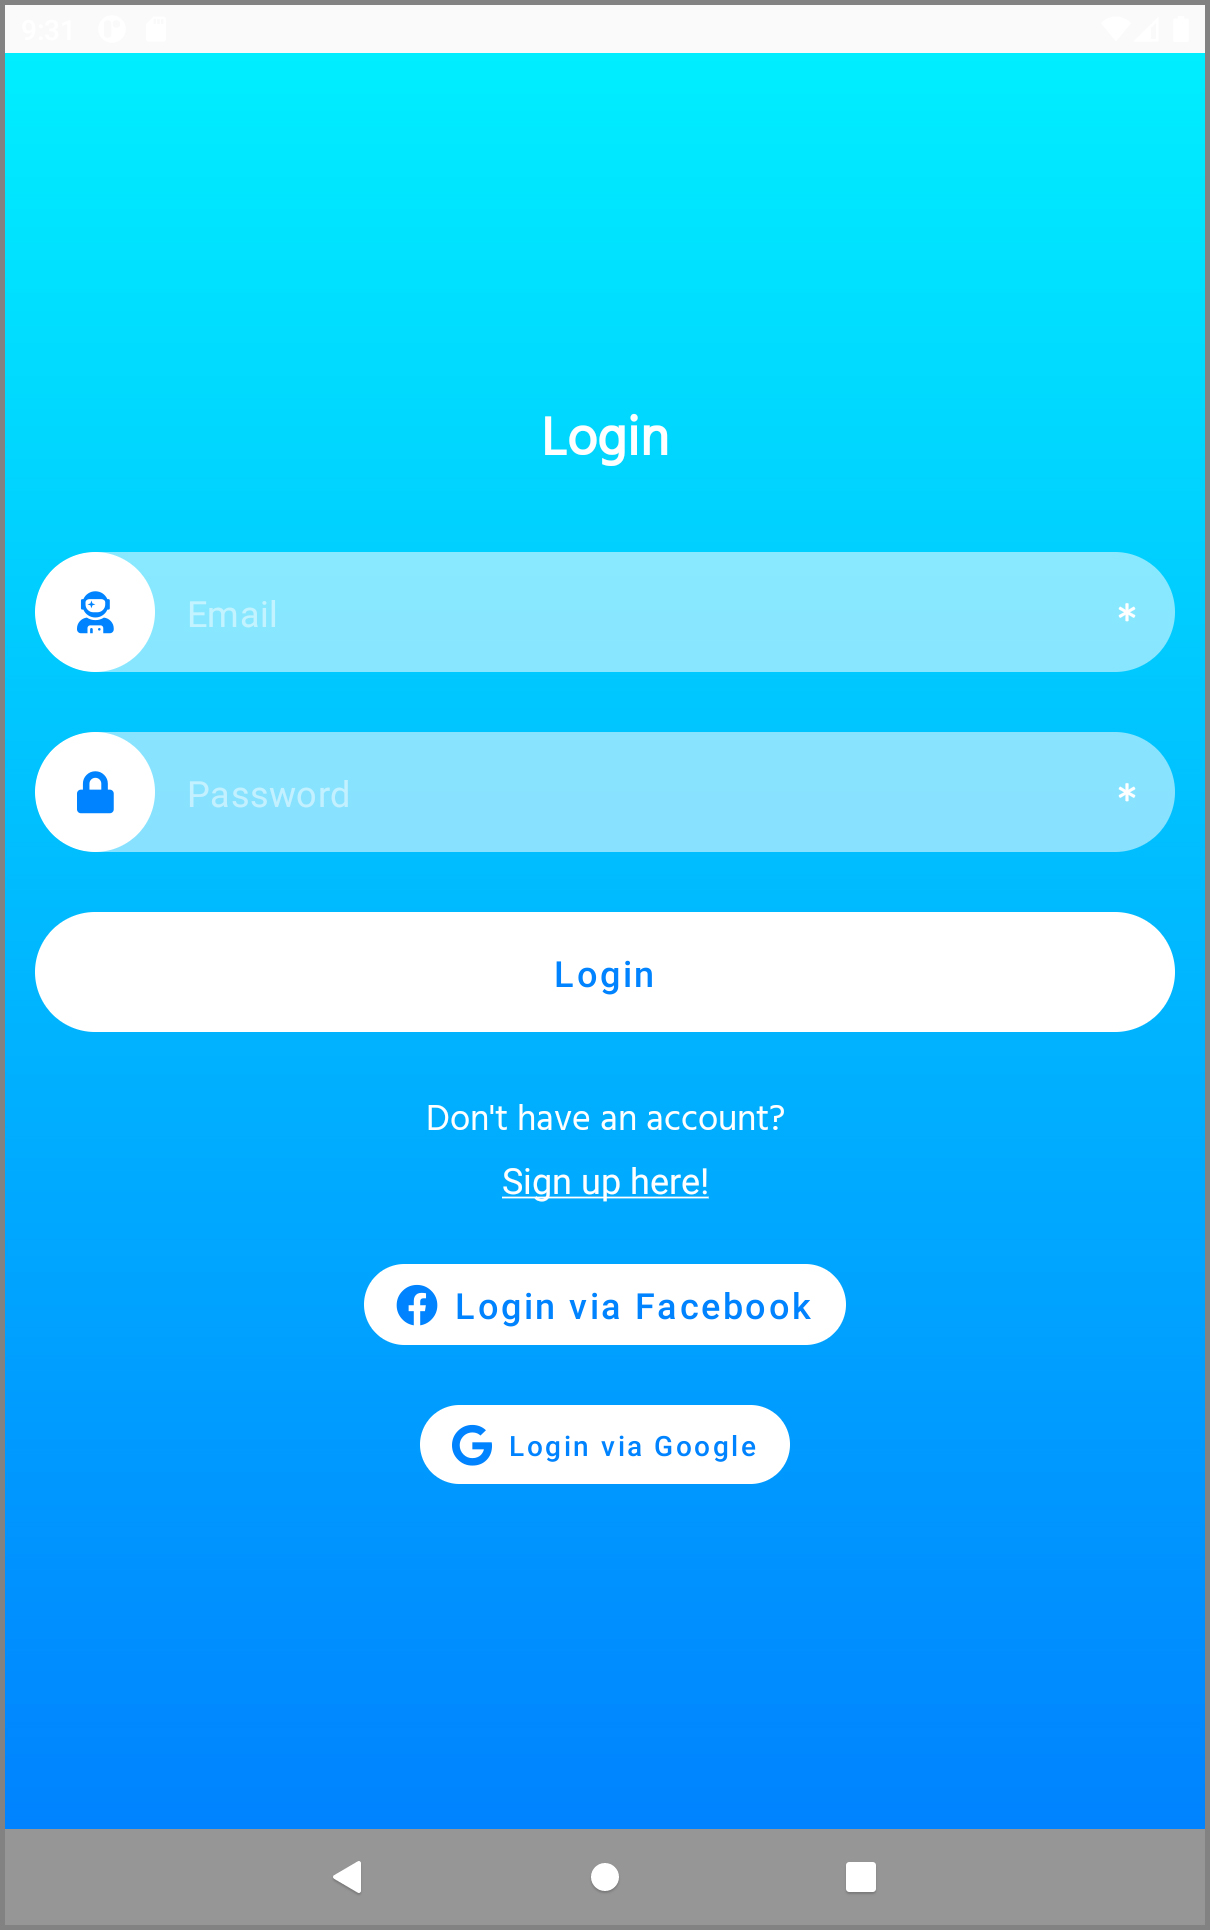
\includegraphics[width=.95\textwidth]{../Images/UI/LoginBig.jpg}
\caption{\label{fig:dbapiuser}\textbf{Login screen - Tablet}}
\end{minipage} 
\begin{minipage}{.45\textwidth}
\centering
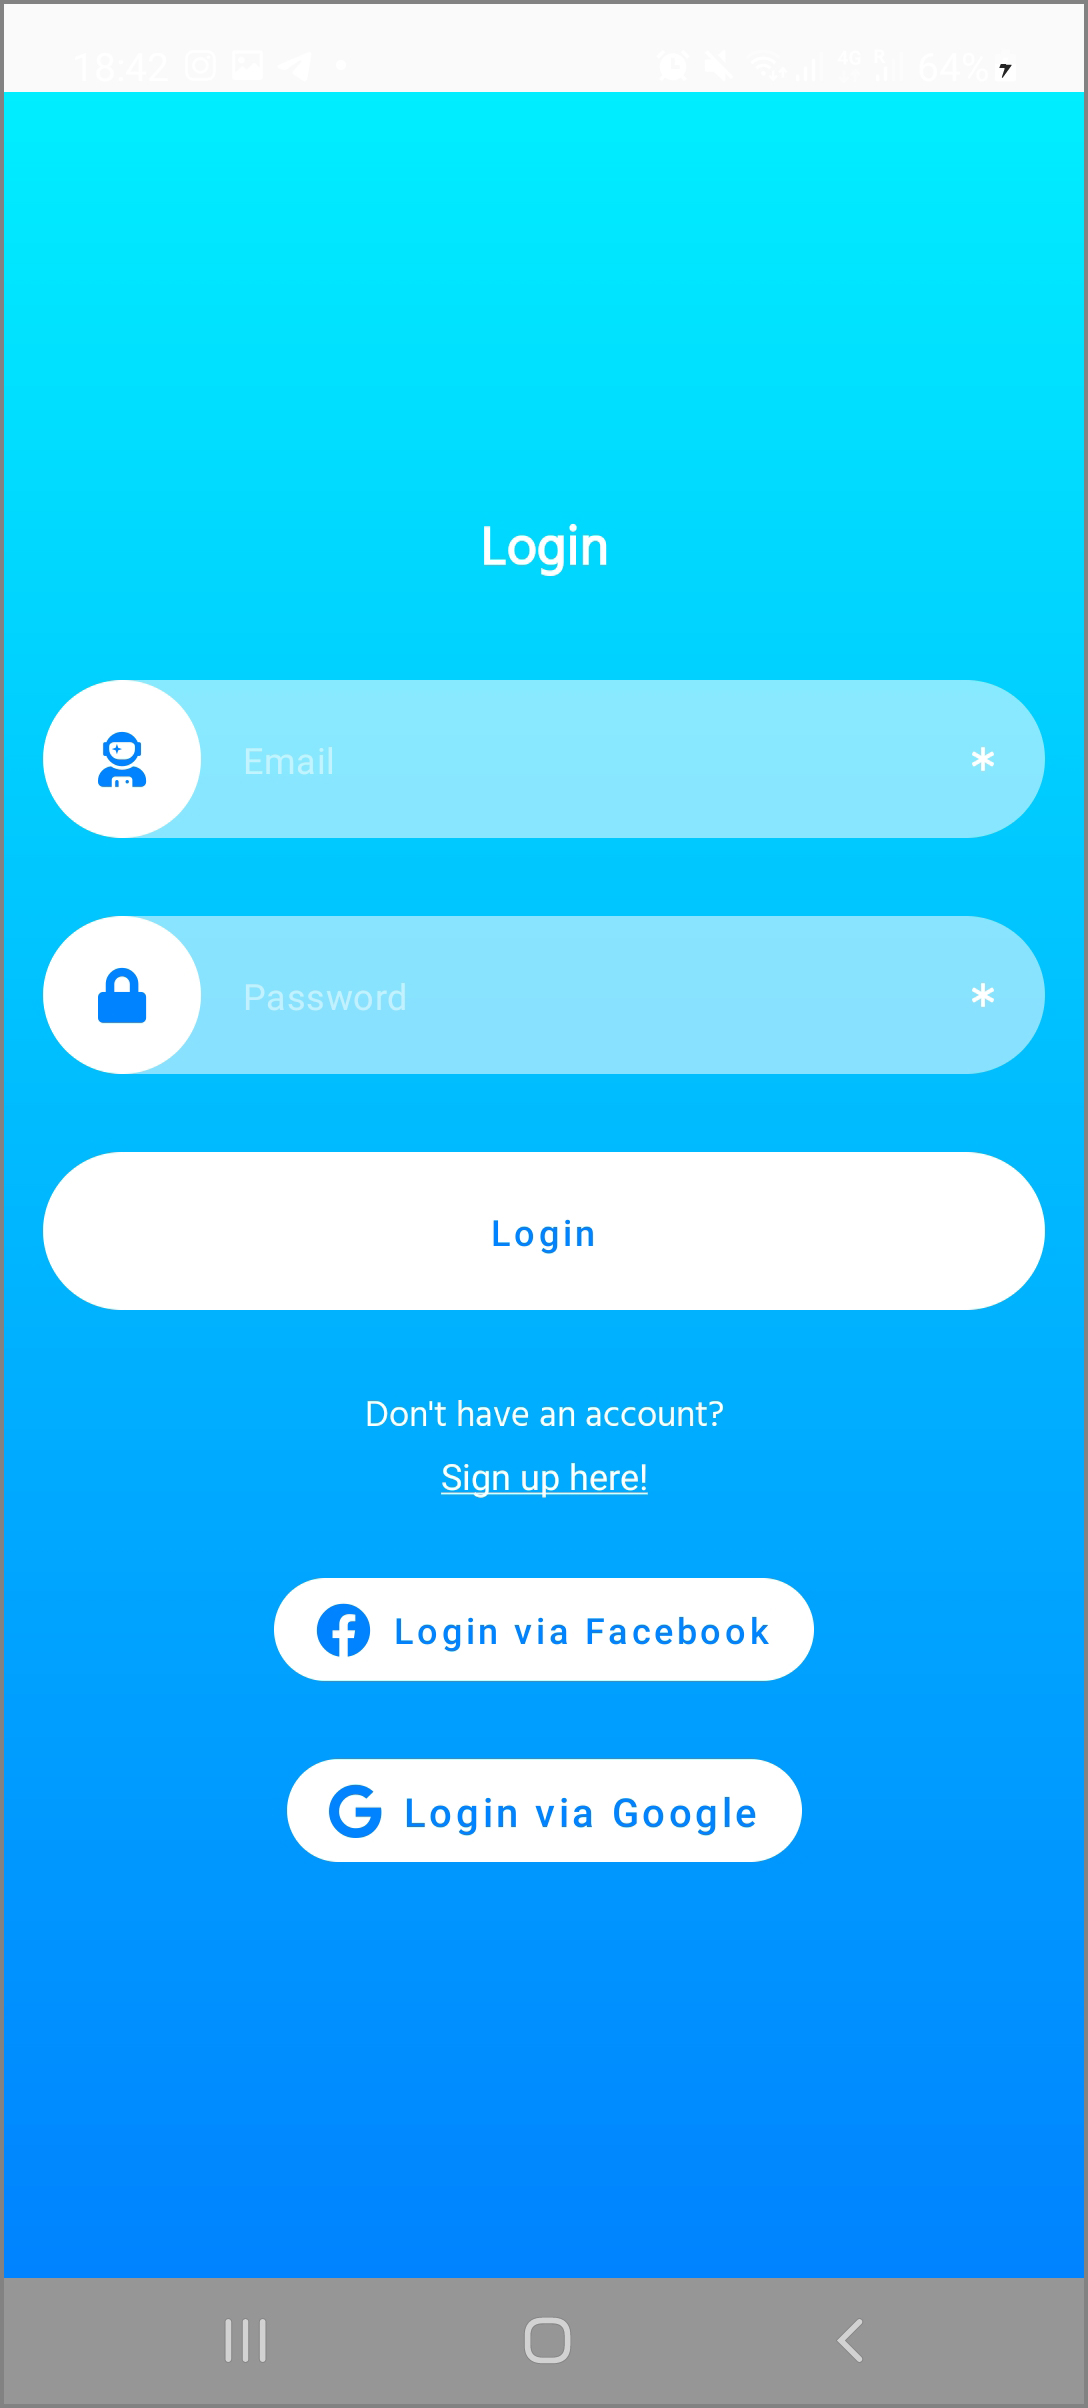
\includegraphics[width=.8\textwidth]{../Images/UI/Login.jpg}
\caption{\label{fig:dbapiuser}\textbf{Login screen - Phone}}
\end{minipage}
\end{figure}
 
\begin{figure}[!htb]
\centering
\begin{minipage}{.45\textwidth}
\centering
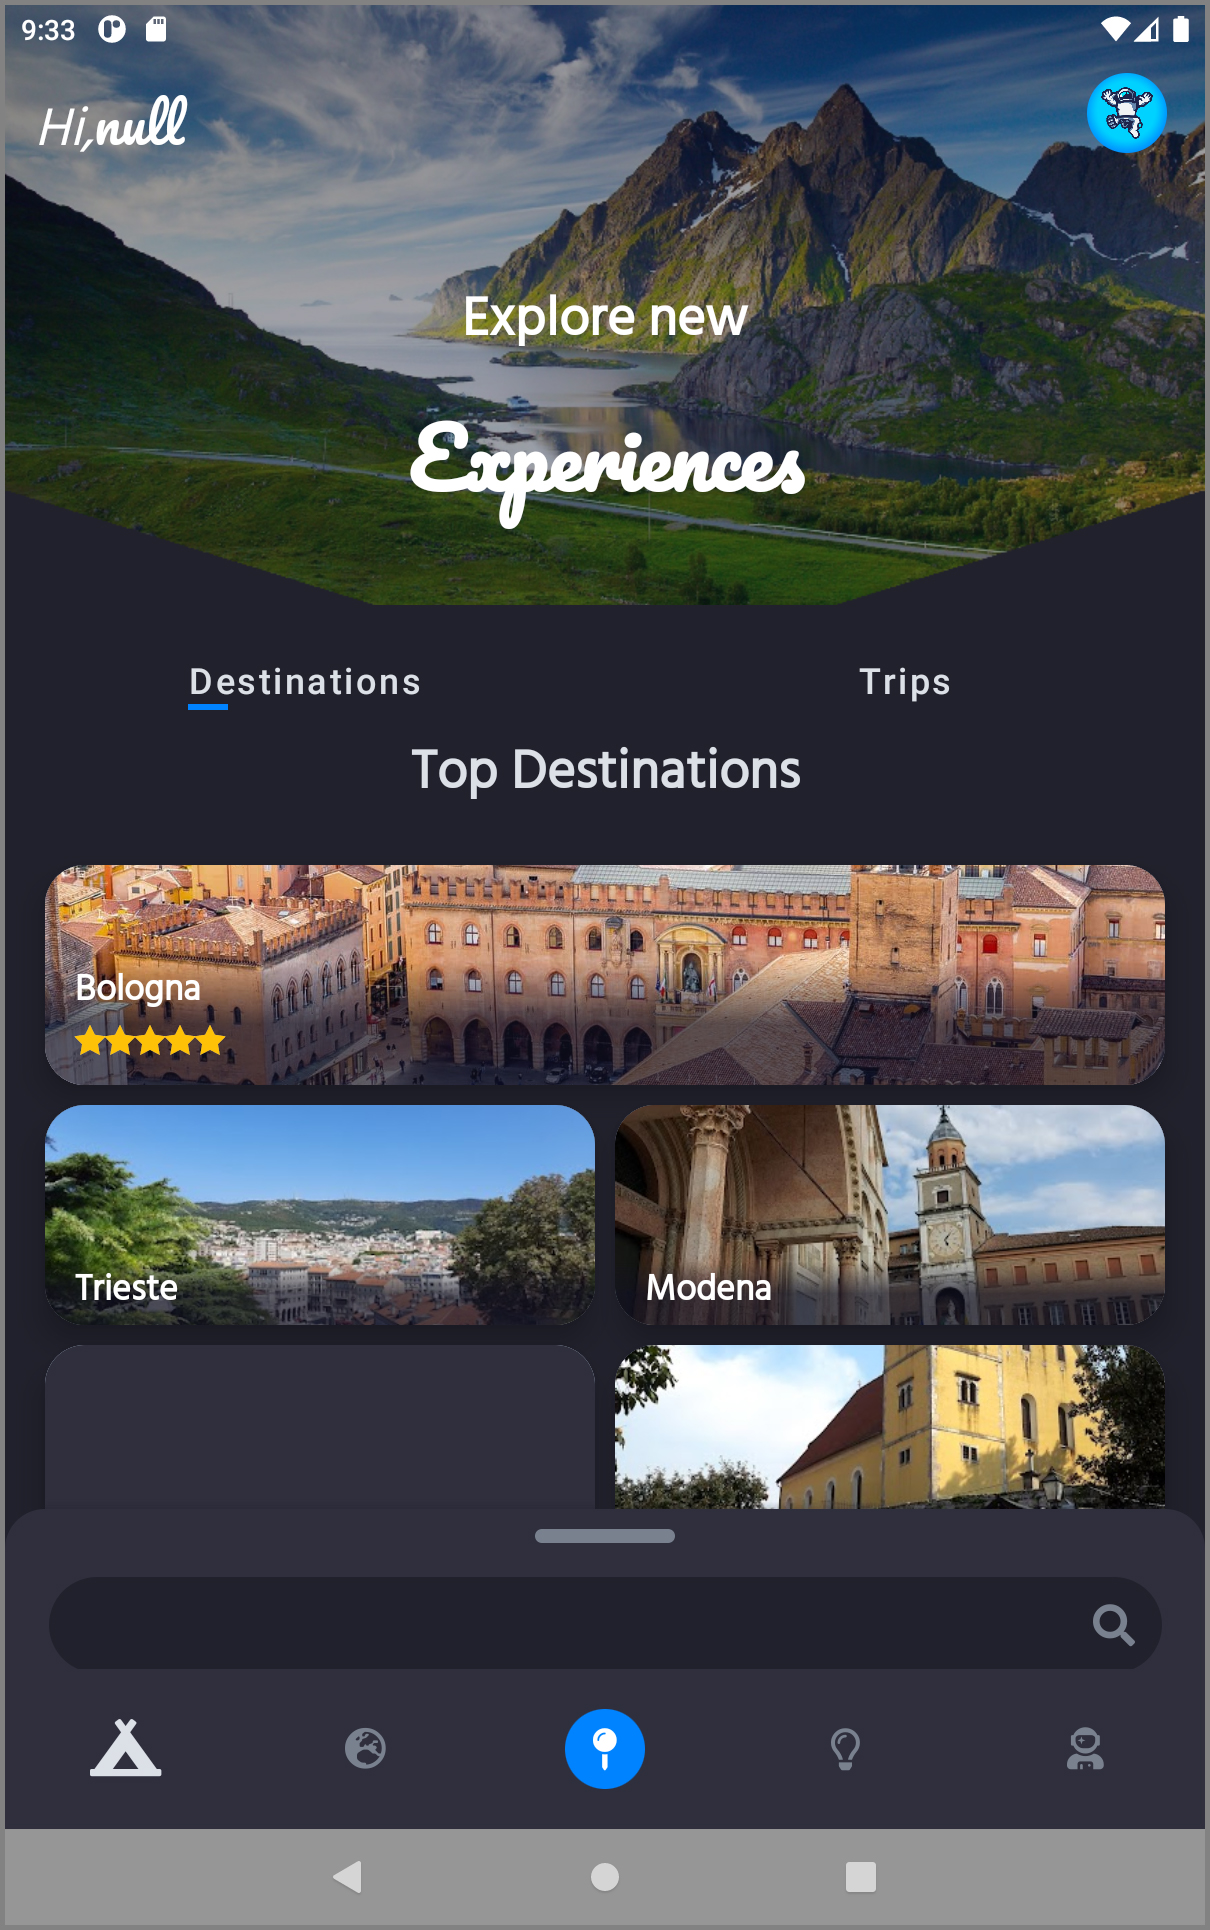
\includegraphics[width=.95\textwidth]{../Images/UI/HomeBig.jpg}
\caption{\label{fig:dbapiuser}\textbf{Home screen - Tablet}}
\end{minipage} 
\begin{minipage}{.45\textwidth}
\centering
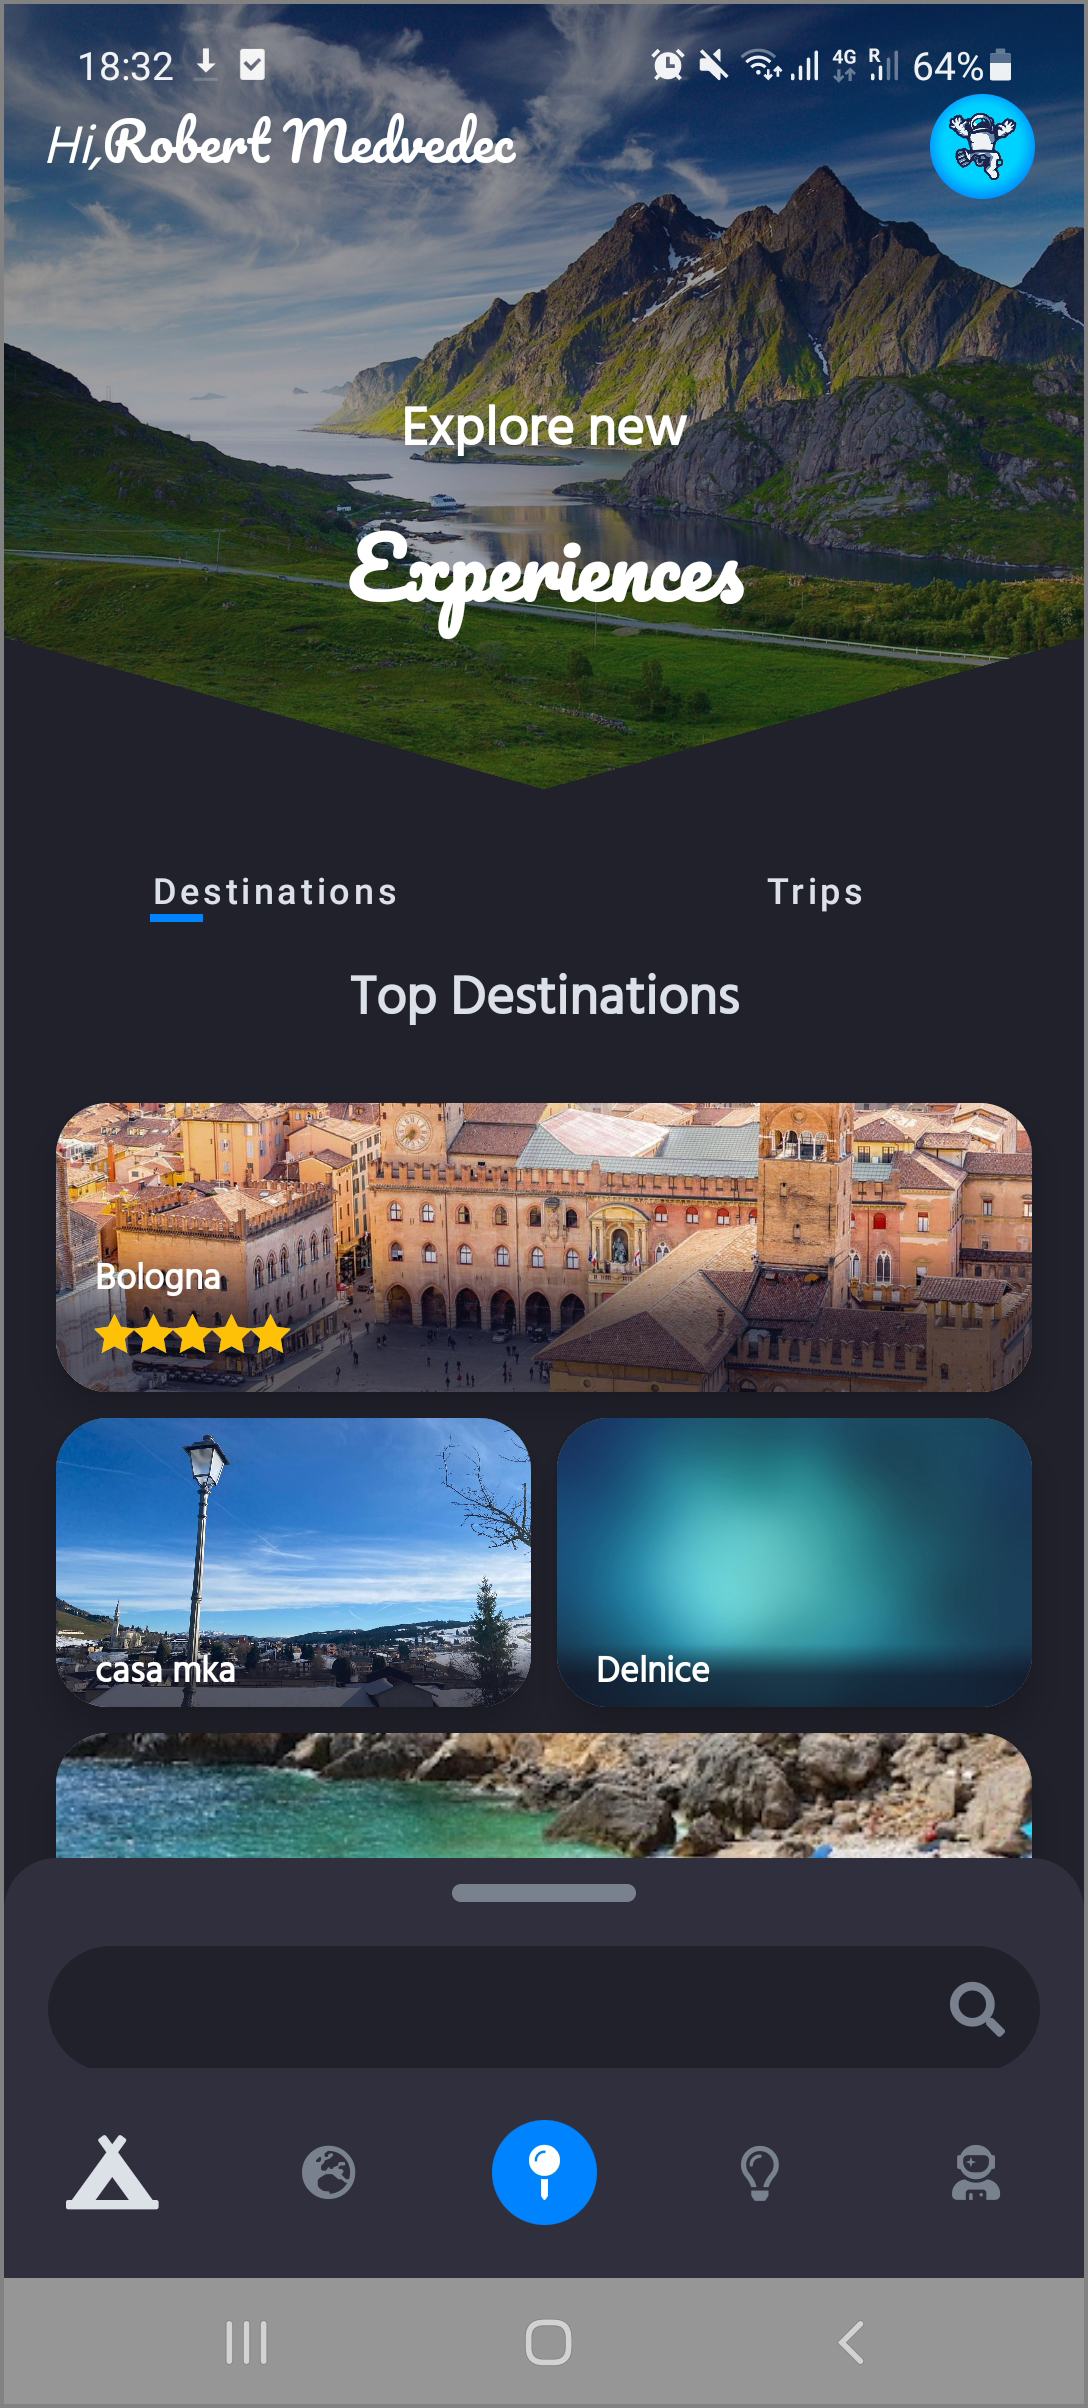
\includegraphics[width=.8\textwidth]{../Images/UI/DestinationsMain.jpg}
\caption{\label{fig:dbapiuser}\textbf{Home screen - phone}}
\end{minipage}
\end{figure} 

\begin{figure}[!htb]
\centering
\begin{minipage}{.45\textwidth}
\centering
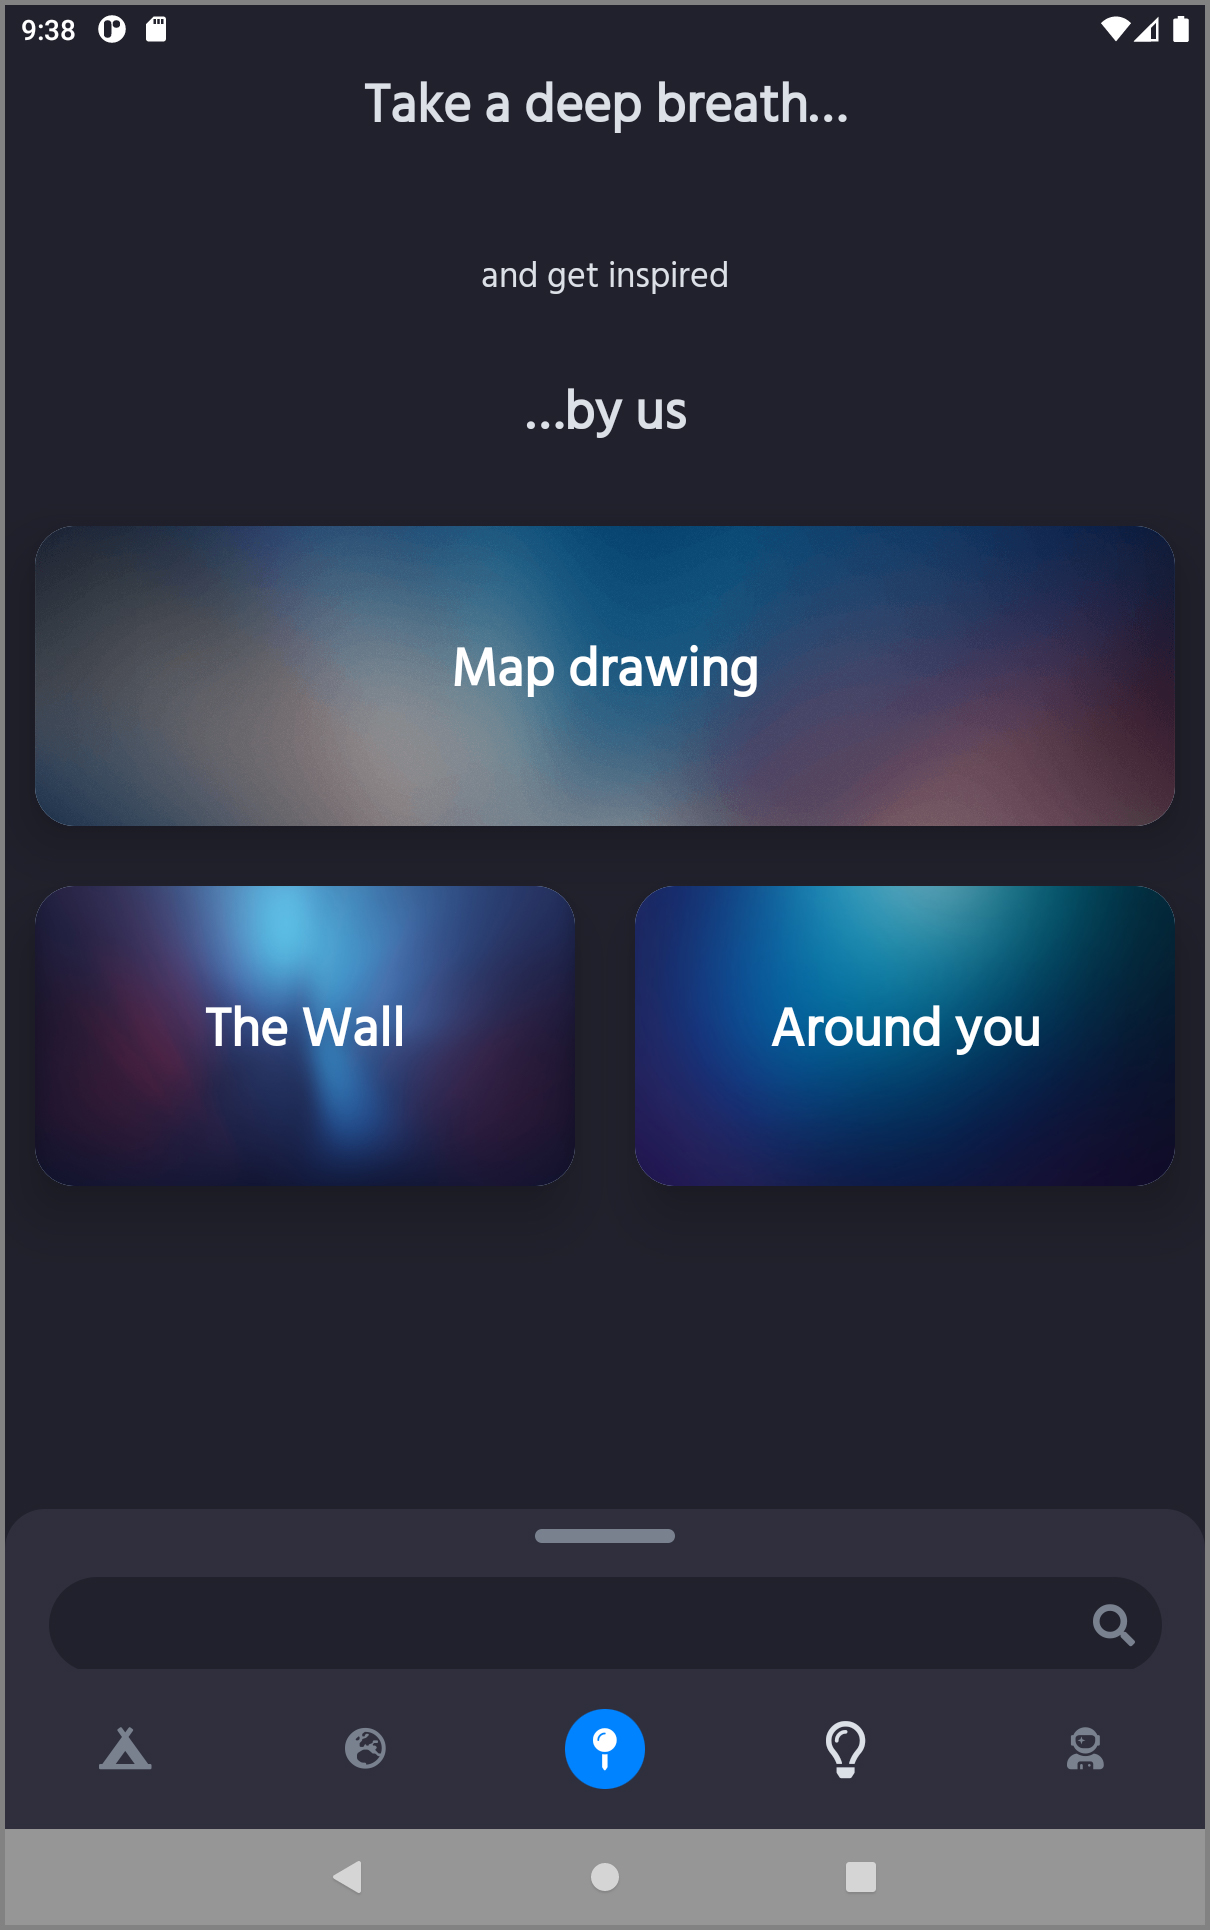
\includegraphics[width=.95\textwidth]{../Images/UI/ExploreBig.jpg}
\caption{\label{fig:dbapiuser}\textbf{Explore screen - Tablet}}
\end{minipage} 
\begin{minipage}{.45\textwidth}
\centering
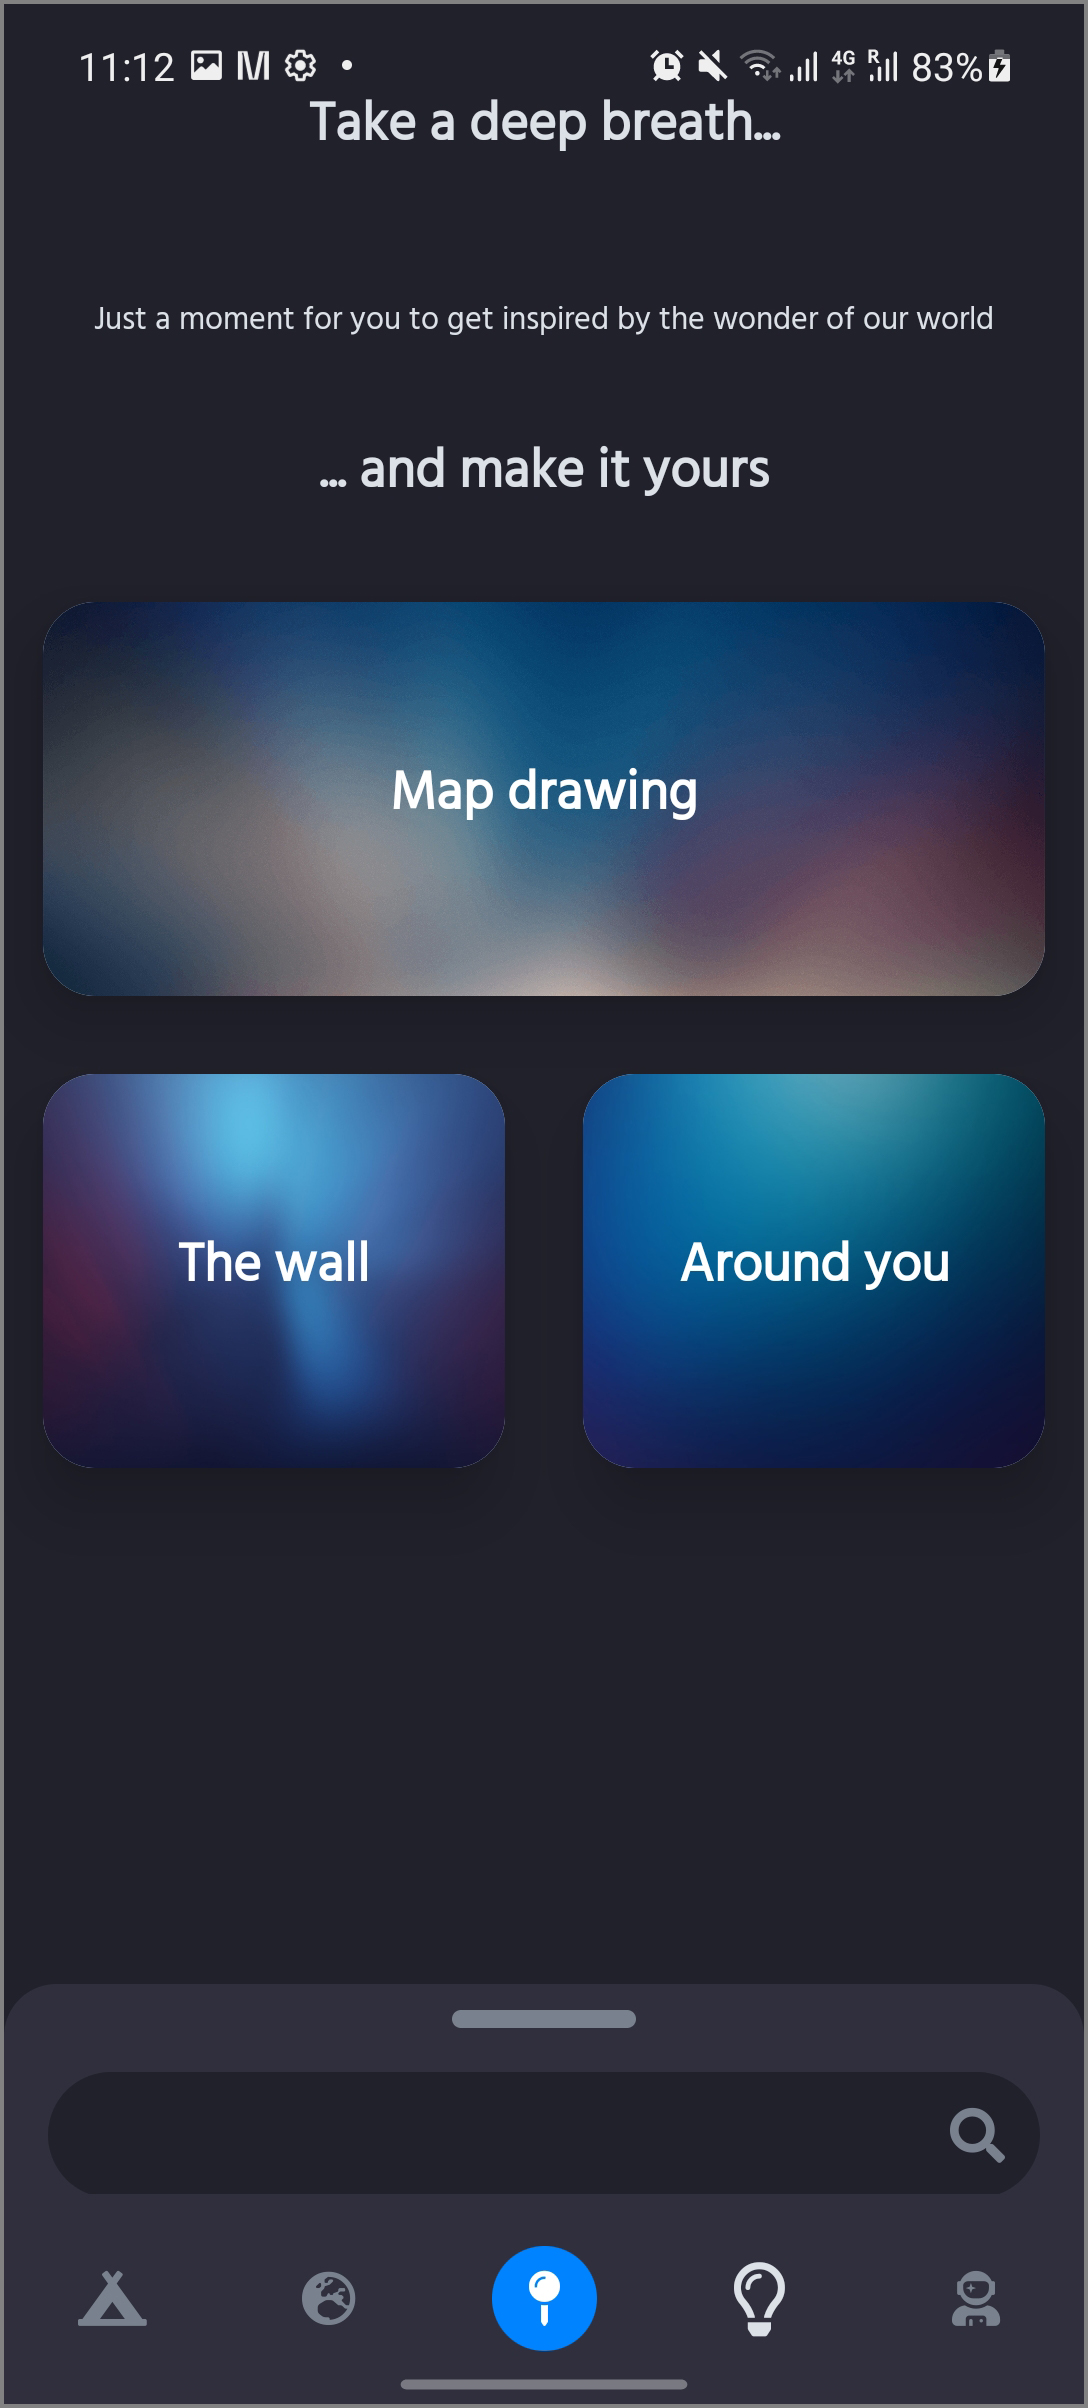
\includegraphics[width=.8\textwidth]{../Images/UI/ExploreDark.jpg}
\caption{\label{fig:dbapiuser}\textbf{Explore screen - Phone}}
\end{minipage}
\end{figure} 

\begin{figure}[!htb]
\centering
\begin{minipage}{.45\textwidth}
\centering
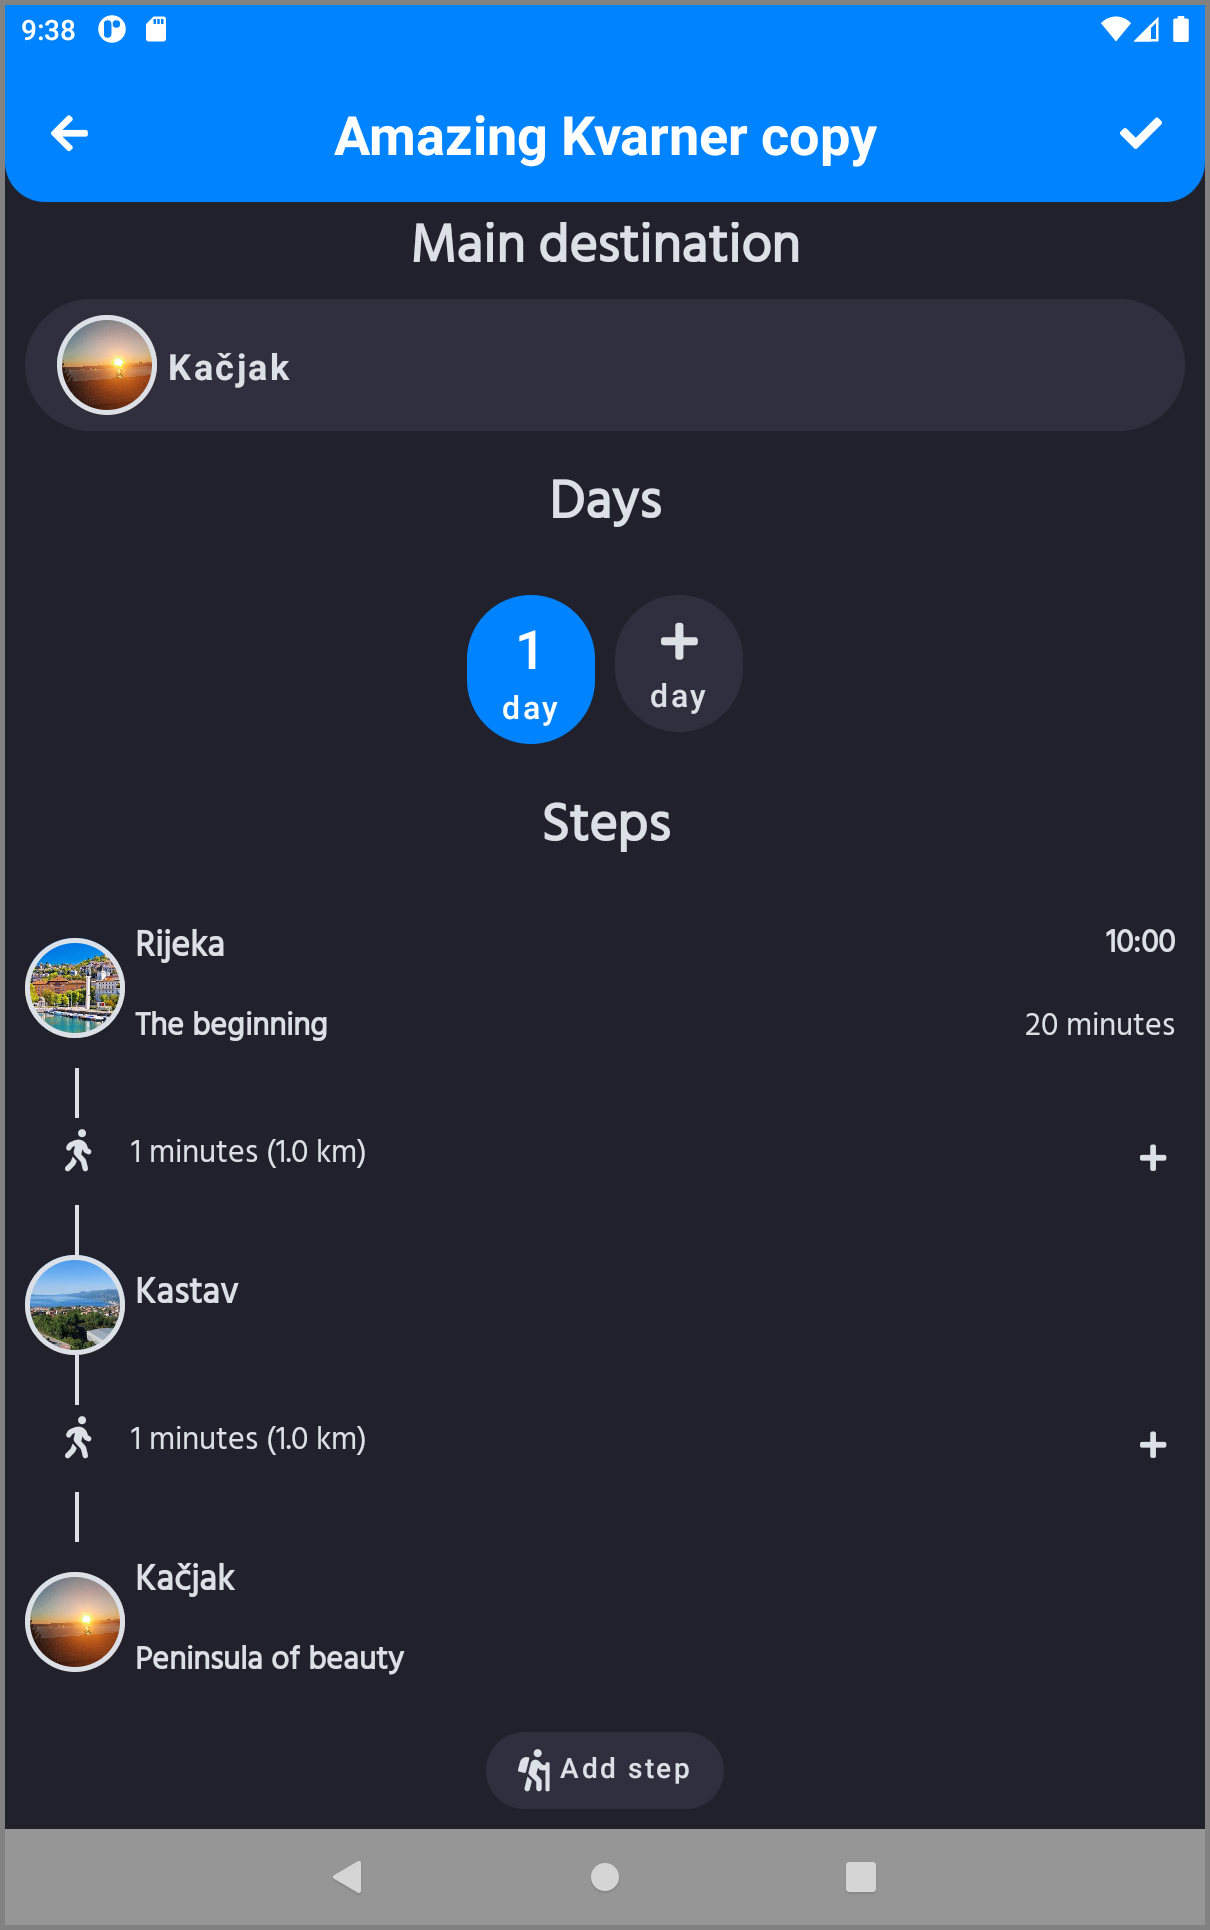
\includegraphics[width=.95\textwidth]{../Images/UI/TripCreateBig.jpg}
\caption{\label{fig:dbapiuser}\textbf{Trip create screen - Tablet}}
\end{minipage} 
\begin{minipage}{.45\textwidth}
\centering
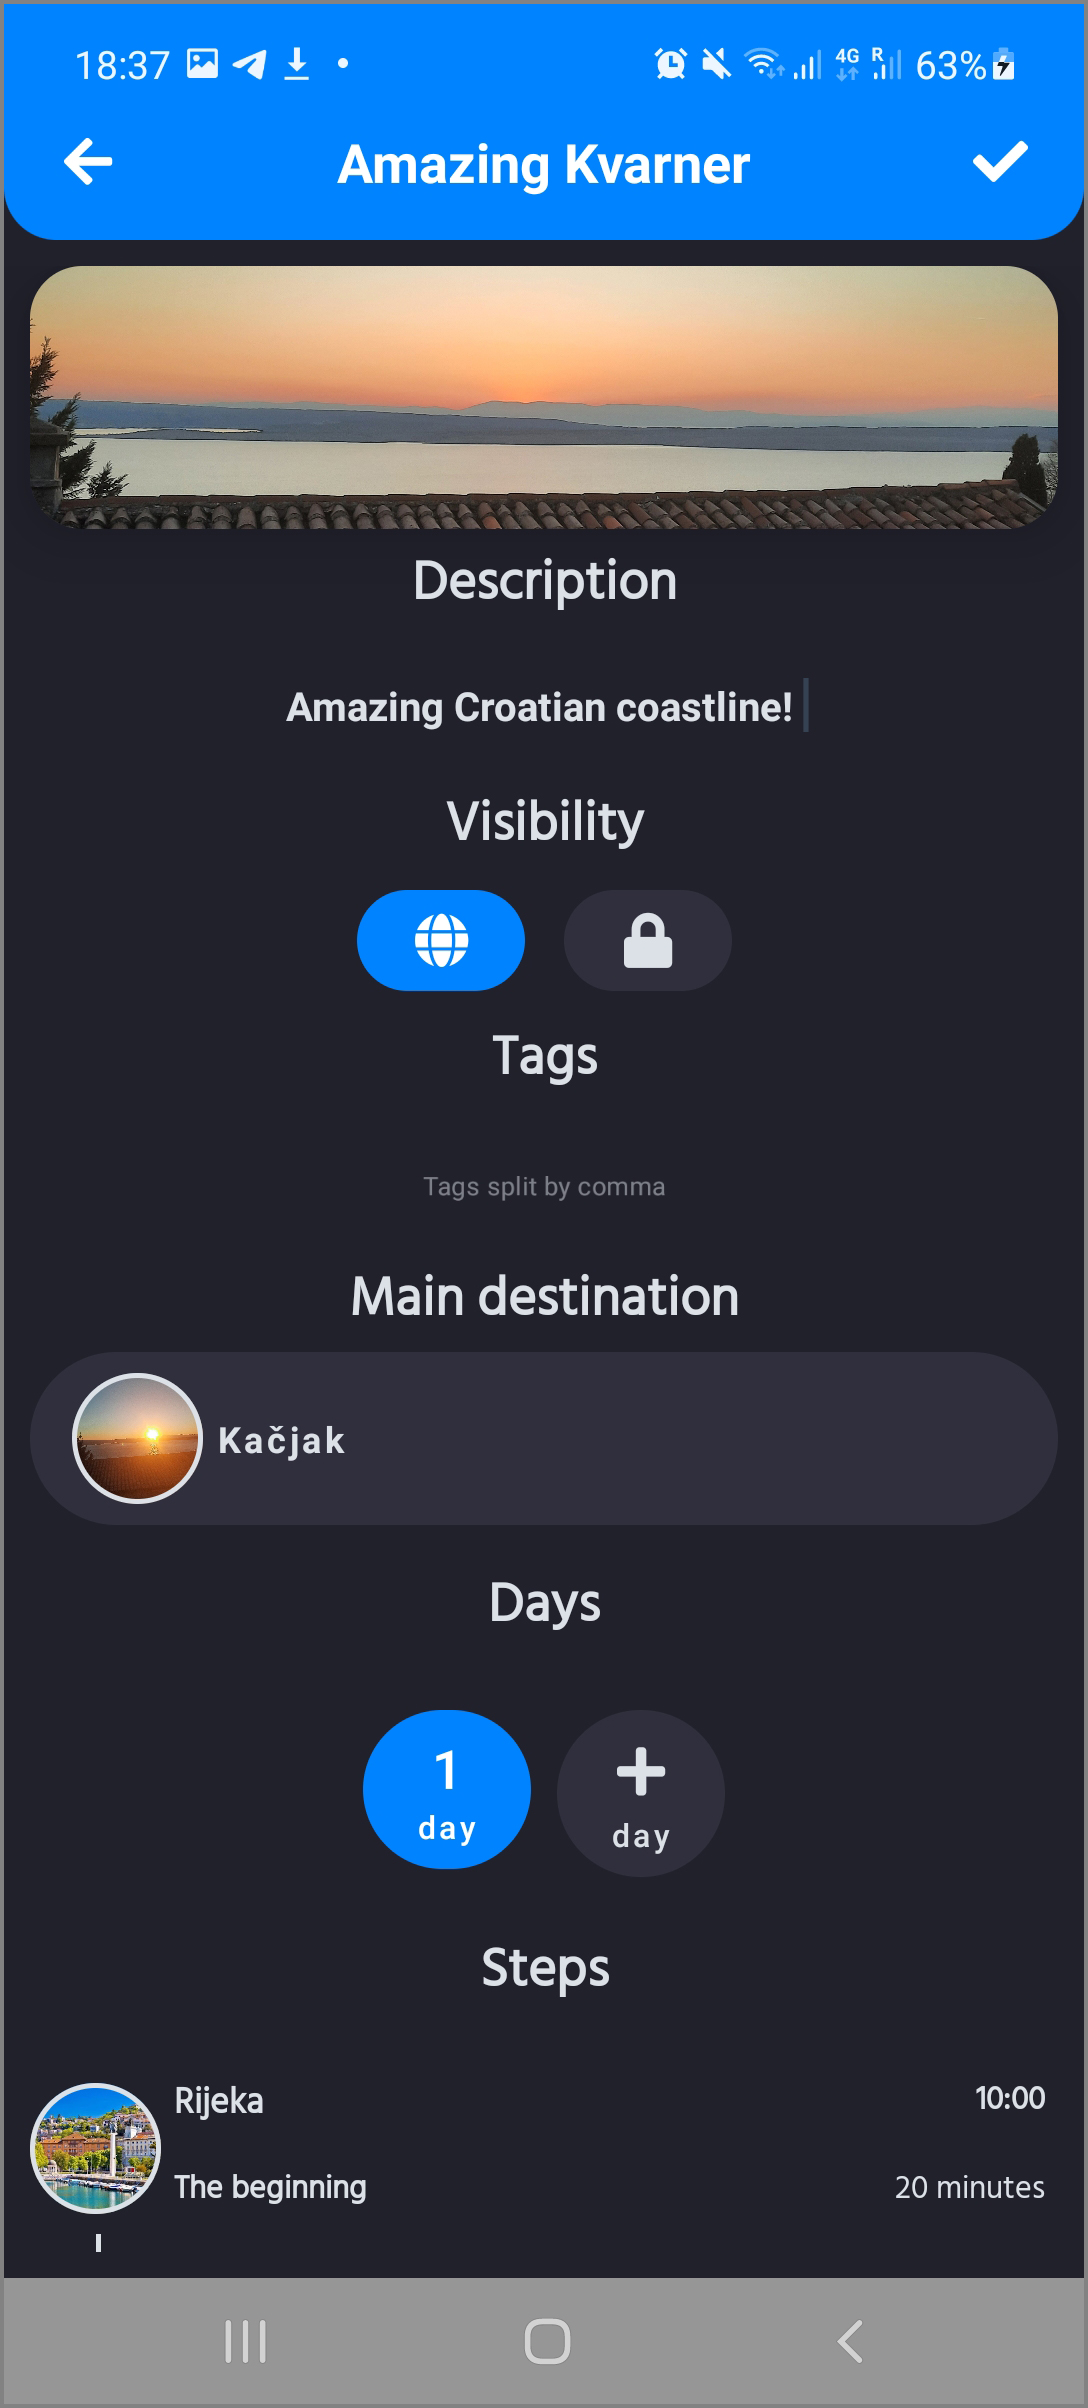
\includegraphics[width=.8\textwidth]{../Images/UI/TripCreateDark.jpg}
\caption{\label{fig:dbapiuser}\textbf{Trip create sreen - Phone}}
\end{minipage}
\end{figure} 

\newpage

%------------------------------------------------------------------------------------------------------------------------------------------------
%\clearpage
%{\color{Blue}{\section{Overall Description}}}
%\label{sect:overview}
%Here you can see how to include an image in your document.

\begin{sidewaysfigure}
\centering
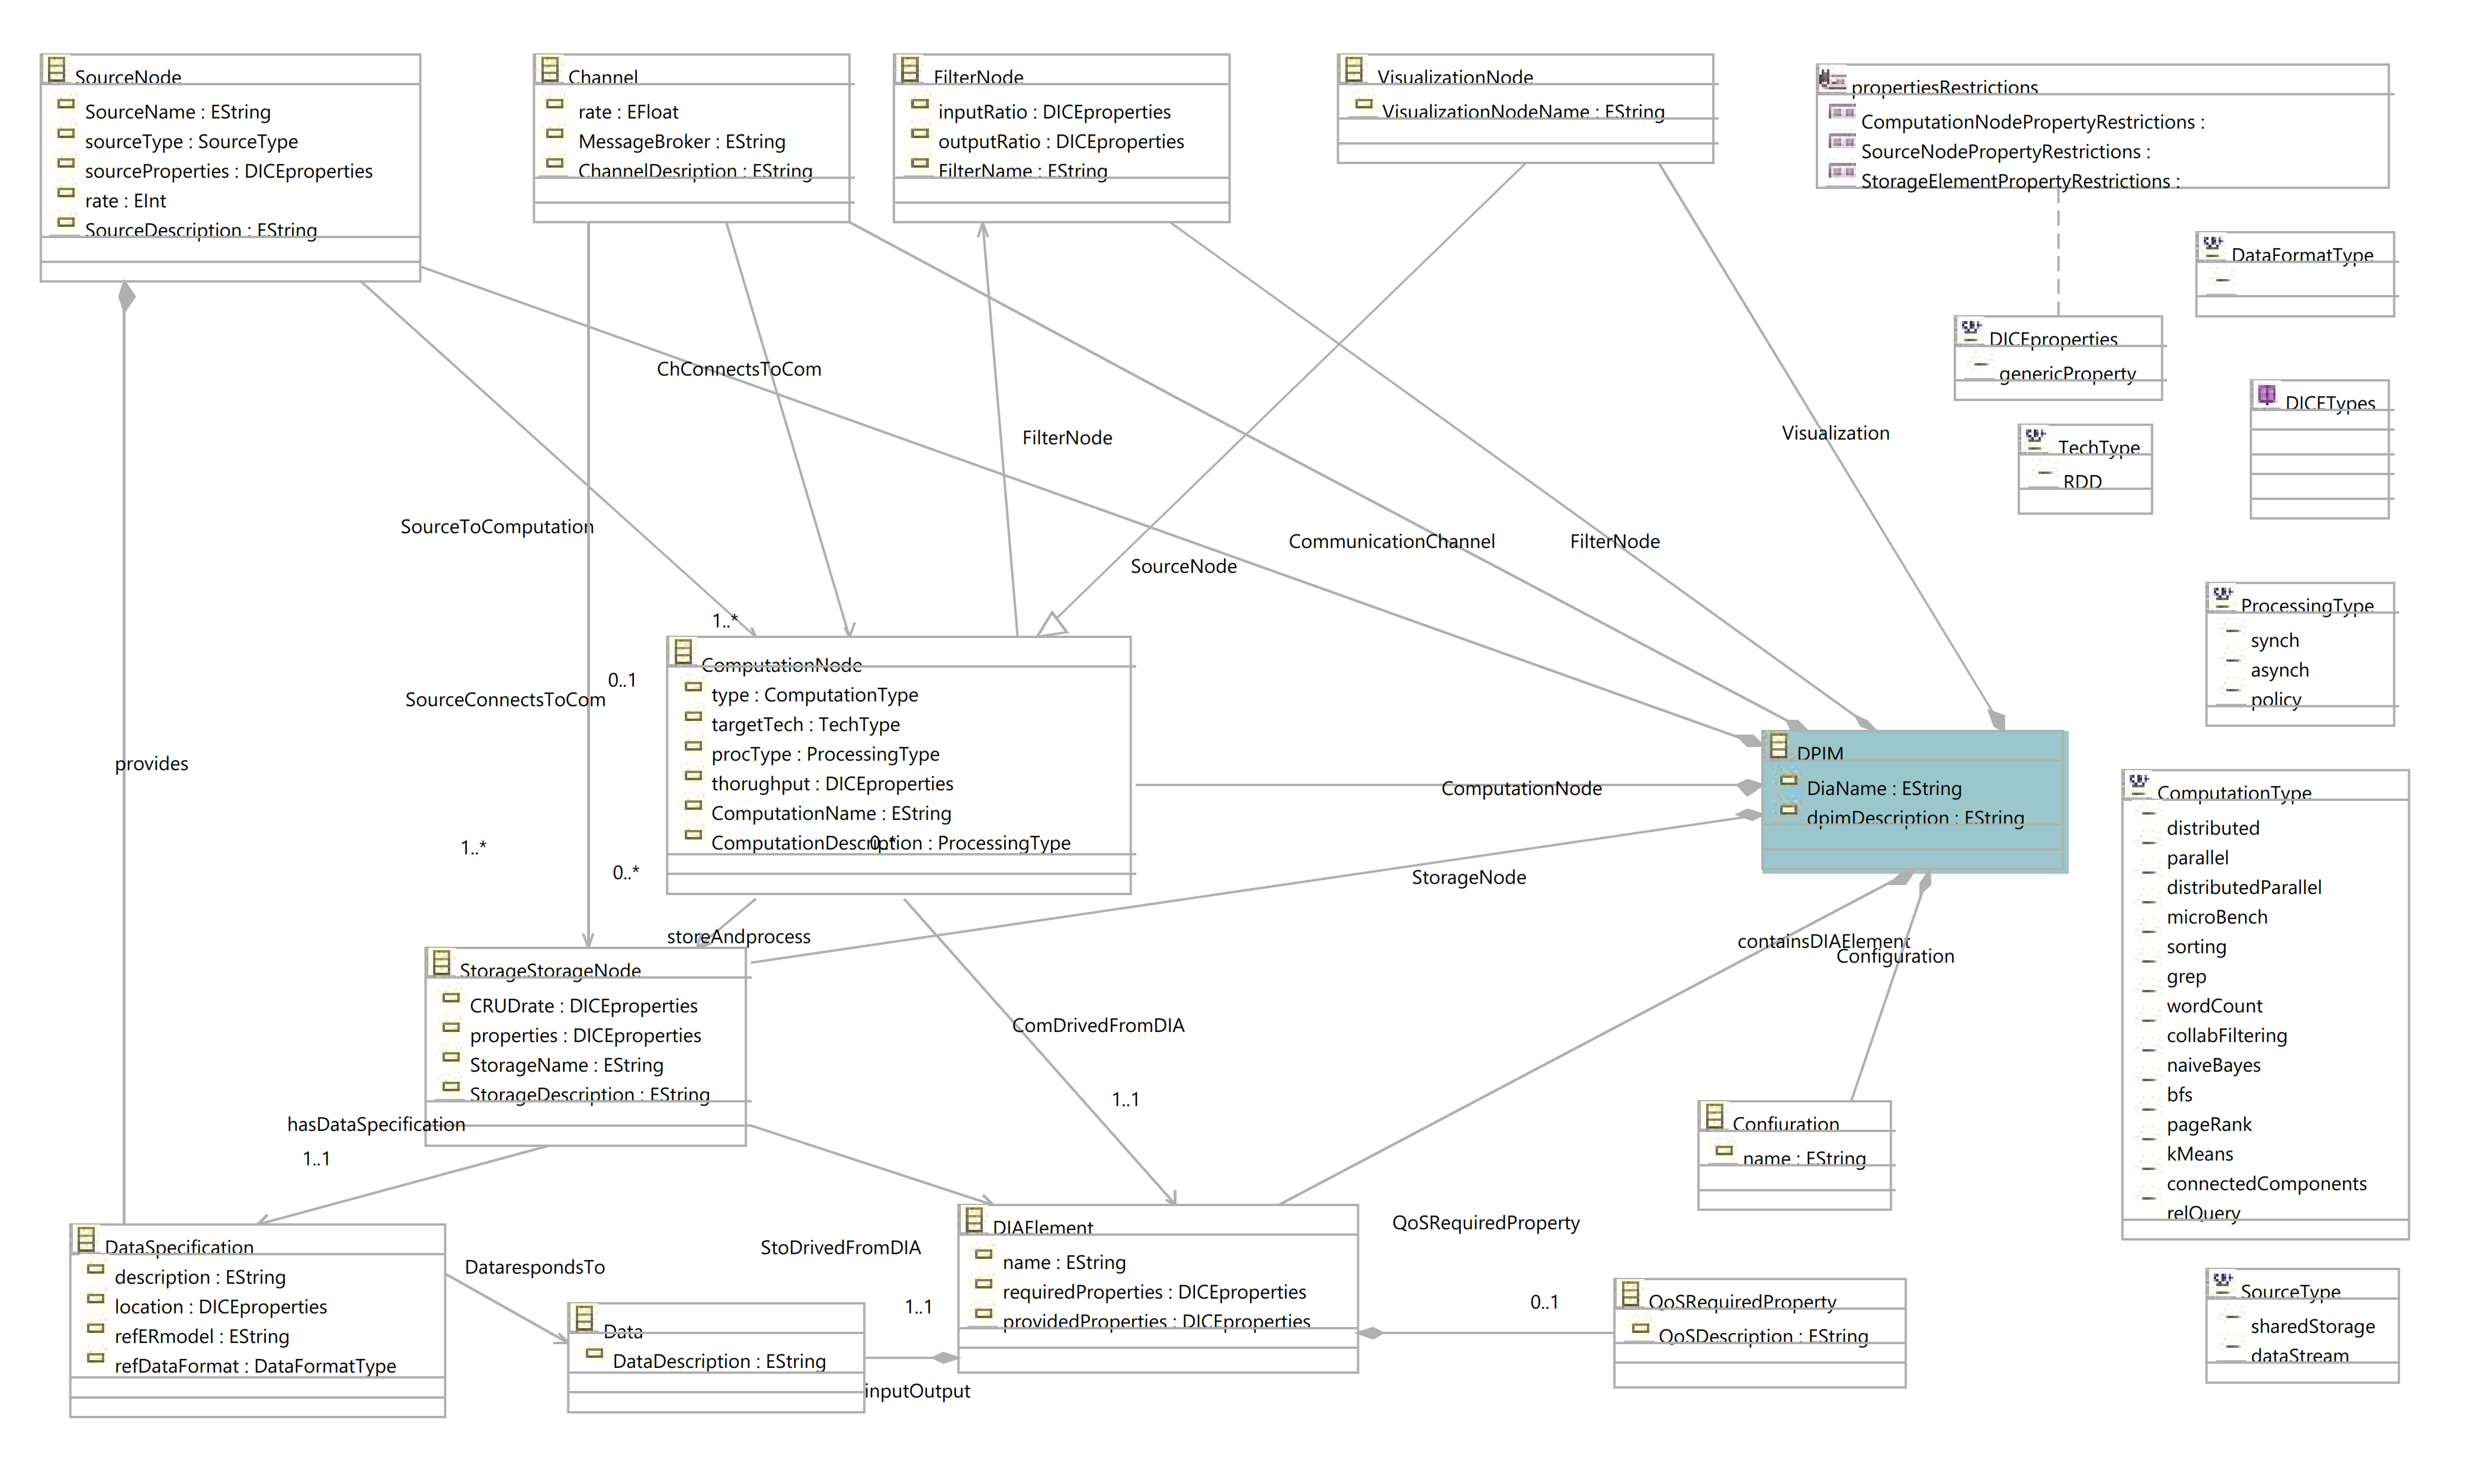
\includegraphics[width=\textwidth]{Images/11.png}
\caption{\label{fig:metamodel}DICE DPIM metamodel.}
\end{sidewaysfigure}

\begin{figure}
\centering
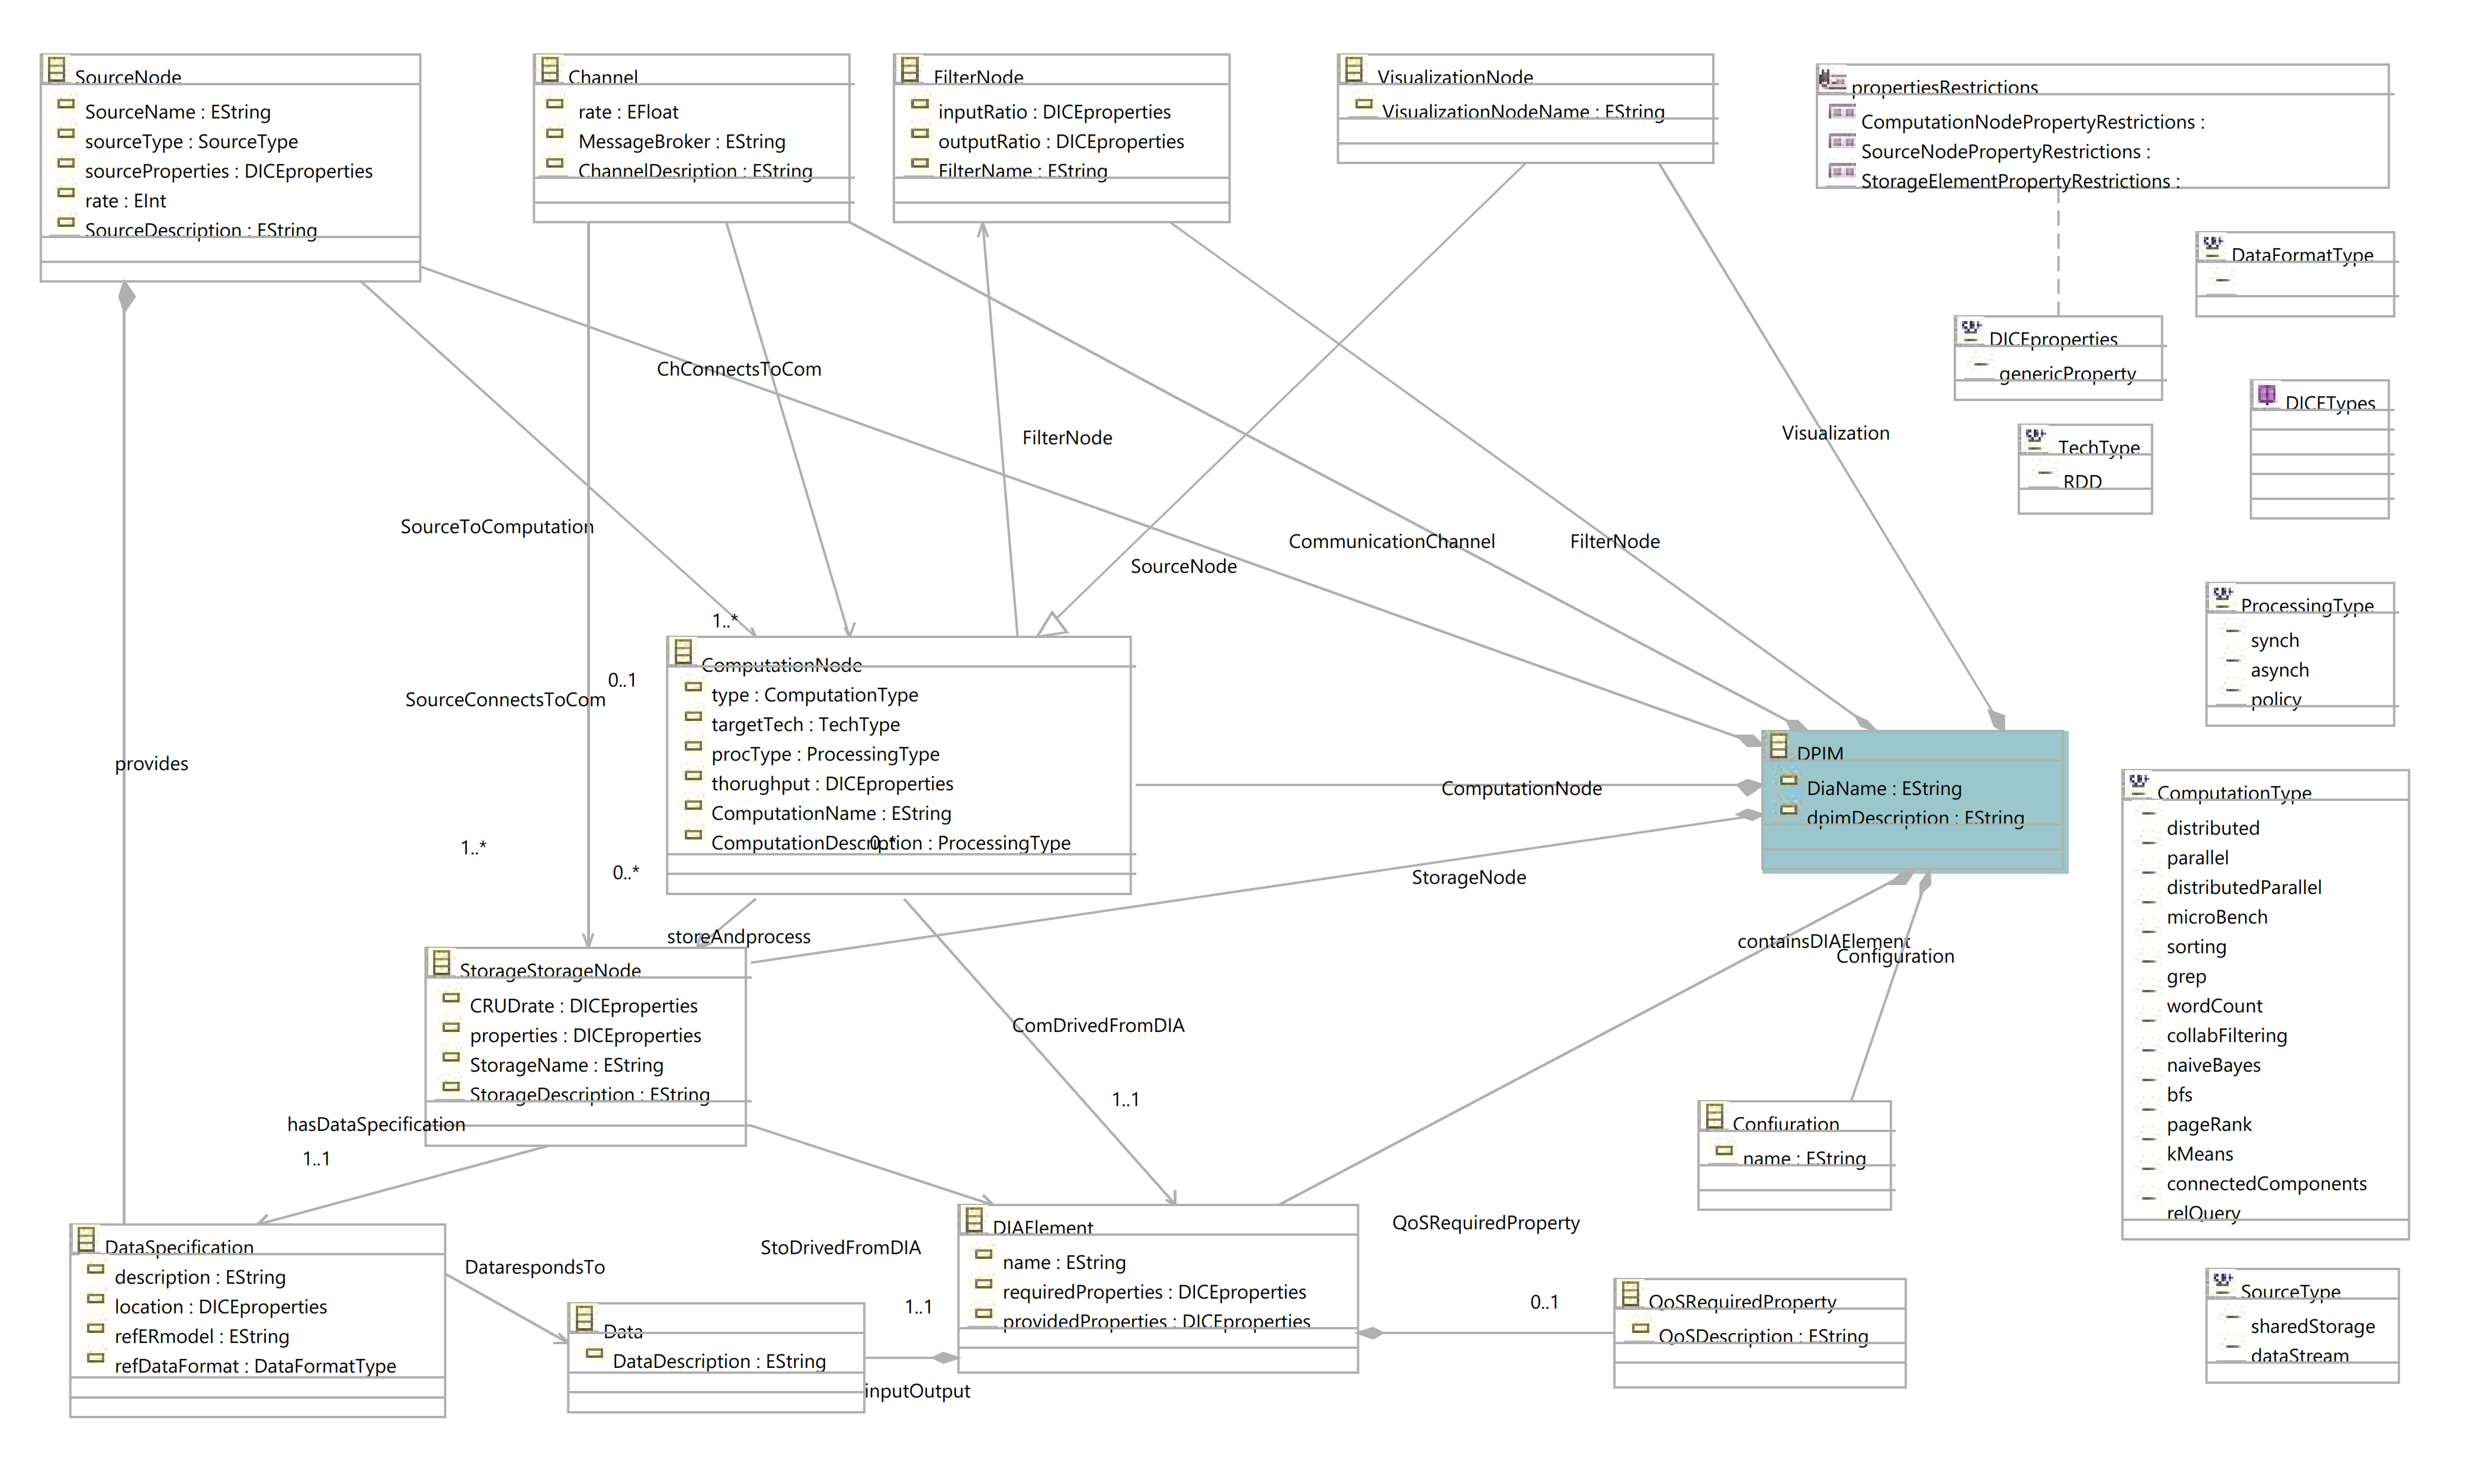
\includegraphics[width=\textwidth]{Images/11.png}
\caption{\label{fig:metamodel2}DICE DPIM metamodel in portrait form.}
\end{figure}

Here is the command to refer to another element (section, figure, table, ...) in the document: \emph{As discussed in Section~\ref{sect:overview} and as shown in Figure~\ref{fig:metamodel}, ...}. Here is how to introduce a bibliographic citation~\cite{DAM}. Bibliographic references should be included in a \texttt{.bib} file. 

Table generation is a bit complicated in Latex. You will soon become proficient, but to start you can rely on tools or external services. See for instance this \href{https://www.tablesgenerator.com}{https://www.tablesgenerator.com}. 


%------------------------------------------------------------------------------------------------------------------------------------------------
%\clearpage
%{\color{Blue}{\section{Specific Requirements}}}
%\label{sect:requirements}
%\subsection{External Interface Requirements}
\subsubsection{User Interfaces}
\hspace{\parindent}The CLup application interface will have to serve two types of users: customers and store managers. Opening screen of the application allows the user to pick a store or to login as a store manager. Depending on the choice, another screen is presented. For a customer, a screen with the options to retrieve a ticket, book a visit or change the store. For a store manager, a screen containing their camera view, and buttons to confirm the scanned ticket, notify the system about a customer exit and to log out of the application. 
\subsubsection{Hardware Interfaces}
\hspace{\parindent}Depending on the current user the CLup application will require access to some hardware interfaces. If the current user is a customer, the application will require the device's camera and if the current user is the store manager the GPS location data will be needed. The application will require no further hardware interfaces.
\subsubsection{Software Interfaces}
\hspace{\parindent}The CLup application will not require any specific software interfaces.
\subsubsection{Communication Interfaces}
\hspace{\parindent}The most important communication will occur between the device and the database. The decision on the specific communication interface which will be used depends on the database, and is, therefore, left to the developers.

\newpage
\subsection{Functional Requirements}
\begin{enumerate}
	\item [\textbf{G1}] Allow a User to "line up"/retrieve a number.
	\begin{enumerate}
		\item [\textbf{G1.1}] Allow a User to retrieve a number through the application.
		\begin{enumerate}
			\item [\textbf{R1}] The user must be able to select a specific store in which they want to do the shopping.
			\item [\textbf{R2}] The user must be able to request a number and a ticket.
			\item [\textbf{R3}] The user must be able to receive a number and a ticket.
		\end{enumerate}
		\item [\textbf{G1.2}] Allow a User to retrieve a number physically from the printer.
		\begin{enumerate}
			\item [\textbf{R4}] The user must be able to physically retrieve a ticket from the printer containing a number and a QR code.		
		\end{enumerate}
		\item [\textbf{D8}] The user has internet connection for the device at all times.
	\end{enumerate}
	\item [\textbf{G2}] Allow a Store Manager to control the entrance of a User via QR code scanning.
	\begin{enumerate}
		\item [\textbf{R5}] The store manager must be able to scan a QR code.
		\item [\textbf{R6}] The store manager must be informed by the application if a user tries to enter the store out of order.
		\item [\textbf{R7}] The store manager must be informed when the capacity of the store is full.
		\item [\textbf{R8}] The store manager must be able to alert the system whenever a customer exits the store.
		\item [\textbf{D6}] The system can correctly save data about enter and exit times of anonymous customers, in order to calculate estimated wait time.
		\item [\textbf{D8}] The user has internet connection for the device at all times.
	\end{enumerate}
	\item [\textbf{G3}] Allow a User to get precise calculations of the wait time.
	\begin{enumerate}
		\item [\textbf{R9}] Allow the user to receive a precise estimation of wait time when retrieving a number.
		\item [\textbf{R10}] The system must provide the user with an estimation of wait time based on data.
		\item [\textbf{D4}] The system can use data about the registered user to calculate estimated wait time.
		\item [\textbf{D6}] The system can correctly save data about enter and exit times of anonymous customers, in order to calculate estimated wait time.
		\item [\textbf{D8}] The user has internet connection for the device at all times.
	\end{enumerate}
	\item [\textbf{G4}] Allow a User to get updates/notifications on the estimated wait time.
	\begin{enumerate}
		\item [\textbf{R11}] The system must be able to update its estimated wait time in real time.
		\item [\textbf{R12}] The system must be able to send an update to the user in specific intervals regarding estimated wait time until it's their turn.
		\item [\textbf{D4}] The system can use data about the registered user to calculate estimated wait time.
		\item [\textbf{D6}] The system can correctly save data about enter and exit times of anonymous customers, in order to calculate estimated wait time.
		\item [\textbf{D8}] The user has internet connection for the device at all times.
	\end{enumerate}
	\item [\textbf{G5}] Allow a User to "book a visit" to the store.
	\begin{enumerate}
		\item [\textbf{G5.1}] Allow a User to "book a visit" to the store without indicating the expected duration of the visit.
		\begin{enumerate}
			\item [\textbf{R13}] The user must be able to request to see all the available timeslots in that specific store.
			\item [\textbf{R14}] The system must be able to provide the user with the list of all available timeslots upon the request.
			\item [\textbf{R15}] The user must be able to select a specific timeslot.
			\item [\textbf{R16}] The user must be able to receive a confirmation of his timeslot reservation, along with a number and a ticket.
			\item [\textbf{R17}] Allow the user to be at most five minutes late for his reservation before canceling his ticket.
		\end{enumerate}
		\item [\textbf{G5.2}] Allow a User to "book a visit" to the store with indicating the expected duration of the visit.
		\begin{enumerate}
			\item [\textbf{R18}] The user must be able to specify expected duration of his visit to the store.
		\end{enumerate}
 		\item [\textbf{D3}] The user's device provides accurate GPS information.
		\item [\textbf{D7}] The system can correctly save data to and pull data from available time slot schema in the database. 
		\item [\textbf{D8}] The user has internet connection for the device at all times.
	\end{enumerate}
	\item [\textbf{G6}] Allow a Store Manager to login to his store manager account with credentials.
	\begin{enumerate}
		\item [\textbf{R19}] The store manager must be provided with the login credentials upon request to the system administrator.
		\item [\textbf{D1}] The store manager's username must be unique. 
		\item [\textbf{D2}] The store manager's password must be secure. 
	\end{enumerate}
\end{enumerate}

\newpage
\begin{table}[]
\centering
\begin{tabular}{|
>{\columncolor[HTML]{EFEFEF}}l |l|l|}
\hline
\cellcolor[HTML]{C0C0C0}\textbf{Requirement, {[}Rn{]}} & \cellcolor[HTML]{C0C0C0}\textbf{Goals, {[}Gn{]}} & \cellcolor[HTML]{C0C0C0}\textbf{Domains, {[}Dn{]}} \\ \hline
R1  & G1.1 & D8         \\ \hline
R2  & G1.1 & D8         \\ \hline
R3  & G1.1 & D8         \\ \hline
R4  & G1.2 & D8         \\ \hline
R5  & G2   & D6, D8     \\ \hline
R6  & G2   & D6, D8     \\ \hline
R7  & G2   & D6, D8     \\ \hline
R8  & G2   & D6, D8     \\ \hline
R9  & G3   & D4, D6, D8 \\ \hline
R10 & G3   & D4, D6, D8 \\ \hline
R11 & G4   & D4, D6, D8 \\ \hline
R12 & G4   & D4, D6, D8 \\ \hline
R13 & G5.1 & D3, D7, D8 \\ \hline
R14 & G5.1 & D3, D7, D8 \\ \hline
R15 & G5.1 & D3, D7, D8 \\ \hline
R16 & G5.1 & D3, D7, D8 \\ \hline
R17 & G5.1 & D3, D7, D8 \\ \hline
R18 & G5.2 & D3, D7, D8 \\ \hline
R19 & G6   & D1, D2     \\ \hline
\end{tabular}
\caption{Mapping table}
\label{tab:my-table}
\end{table}
\subsection{Performance Requirements}



%------------------------------------------------------------------------------------------------------------------------------------------------
%\clearpage
%{\color{Blue}{\section{Formal Analysis Using Alloy}}}
%\label{sect:alloy}
%Organize this section according to the rules defined in the project description. 


%------------------------------------------------------------------------------------------------------------------------------------------------
%\clearpage
%{\color{Blue}{\section{Effort Spent}}}
%\label{sect:effort}
%Provide here information about how much effort each group member spent in working at this document. We would appreciate details here.



%------------------------------------------------------------------------------------------------------------------------------------------------
%\clearpage
%\addcontentsline{toc}{section}{References}
%\bibliographystyle{plain}
%\bibliography{main}
%------------------------------------------------------------------------------------------------------------------------------------------------




\end{document}
